\documentclass[11pt,a4paper,twoside,openright]{report}
\usepackage[a4paper,hmargin=2.8cm,vmargin=2.0cm,includeheadfoot]{geometry}

\usepackage[nottoc]{tocbibind}

\usepackage[xindy={glsnumbers=false}, nonumberlist, nopostdot, nogroupskip]{glossaries}
\usepackage{enumitem}
\makeglossaries

\newcommand{\reporttitle}{Mixed Traffic Simulation for Autonomous Systems in Shared Spaces}
\newcommand{\reportauthor}{Frederik Tobias Hillier}
\newcommand{\reporttype}{Final Year Project 2021}
\newcommand{\cid}{01412520}

\newcommand{\supervisor}{Prof Yiannis K. Demiris}
\newcommand{\supervisorassistant}{Dr Xingchen Zhang}
\newcommand{\secondmarker}{Prof Deniz Gunduz}


% include files that load packages and define macros
%%%%%%%%%%%%%%%%%%%%%%%%%%%%%%%%%%%%%%%%%
% University Assignment Title Page 
% LaTeX Template
% Version 1.0 (27/12/12)
%
% This template has been downloaded from:
% http://www.LaTeXTemplates.com
%
% Original author:
% WikiBooks (http://en.wikibooks.org/wiki/LaTeX/Title_Creation)
%
% License:
% CC BY-NC-SA 3.0 (http://creativecommons.org/licenses/by-nc-sa/3.0/)
% 
% Instructions for using this template:
% This title page is capable of being compiled as is. This is not useful for 
% including it in another document. To do this, you have two options: 
%
% 1) Copy/paste everything between \begin{document} and \end{document} 
% starting at \begin{titlepage} and paste this into another LaTeX file where you 
% want your title page.
% OR
% 2) Remove everything outside the \begin{titlepage} and \end{titlepage} and 
% move this file to the same directory as the LaTeX file you wish to add it to. 
% Then add \input{./title_page_1.tex} to your LaTeX file where you want your
% title page.
%
%----------------------------------------------------------------------------------------
%	PACKAGES AND OTHER DOCUMENT CONFIGURATIONS
%----------------------------------------------------------------------------------------
\usepackage{ifxetex}
\usepackage{textpos}
\usepackage{natbib}
\usepackage{kpfonts}
\usepackage[a4paper,hmargin=2.8cm,vmargin=2.0cm,includeheadfoot]{geometry}
\usepackage{ifxetex}
\usepackage{stackengine}
\usepackage{tabularx,longtable,multirow,subfigure,caption}%hangcaption
\usepackage{fncylab} %formatting of labels
\usepackage{fancyhdr}
\usepackage{color}
\usepackage[tight,ugly]{units}
\usepackage{url}
\usepackage{float}
\usepackage[english]{babel}
\usepackage{amsmath}
\usepackage{graphicx}
\usepackage[colorinlistoftodos]{todonotes}
\usepackage{dsfont}
\usepackage{epstopdf} % automatically replace .eps with .pdf in graphics
\usepackage{natbib}
\usepackage{backref}
\usepackage{array}
\usepackage{latexsym}
\usepackage{etoolbox}

\usepackage[english]{babel}
\usepackage[utf8x]{inputenc}

\usepackage{enumerate} % for numbering with [a)] format 

\bibpunct{[}{]}{,}{n}{,}{,}


%%% HEAD %%%
\fancyhf{}
\fancyhead[R]{\leftmark}
\usepackage{lastpage}
\fancyfoot[C]{\thepage} %/\pageref{LastPage}}



\ifxetex
\usepackage{fontspec}
\setmainfont[Scale=.8]{OpenDyslexic-Regular}
\else
\usepackage[pdftex,pagebackref,hypertexnames=false,colorlinks]{hyperref} % provide links in pdf
\hypersetup{pdftitle={},
  pdfsubject={}, 
  pdfauthor={\reportauthor},
  pdfkeywords={}, 
  pdfstartview=FitH,
  pdfpagemode={UseOutlines},% None, FullScreen, UseOutlines
  bookmarksnumbered=true, bookmarksopen=true, colorlinks,
    citecolor=black,%
    filecolor=black,%
    linkcolor=black,%
    urlcolor=black}
\usepackage[all]{hypcap}
\fi

\usepackage{tcolorbox}

% various theorems
\usepackage{ntheorem}
\theoremstyle{break}
\newtheorem{lemma}{Lemma}
\newtheorem{theorem}{Theorem}
\newtheorem{remark}{Remark}
\newtheorem{definition}{Definition}
\newtheorem{proof}{Proof}

% example-environment
\newenvironment{example}[1][]
{ 
\vspace{4mm}
\noindent\makebox[\linewidth]{\rule{\hsize}{1.5pt}}
\textbf{Example #1}\\
}
{ 
\noindent\newline\makebox[\linewidth]{\rule{\hsize}{1.0pt}}
}



%\renewcommand{\rmdefault}{pplx} % Palatino
% \renewcommand{\rmdefault}{put} % Utopia

\ifxetex
\else
\renewcommand*{\rmdefault}{bch} % Charter
\renewcommand*{\ttdefault}{cmtt} % Computer Modern Typewriter
%\renewcommand*{\rmdefault}{phv} % Helvetica
%\renewcommand*{\rmdefault}{iwona} % Avant Garde
\fi

\setlength{\parindent}{0em}  % indentation of paragraph

%\setlength{\headheight}{14.5pt}
\pagestyle{fancy}
%\fancyfoot[ER,OL]{\thepage}%Page no. in the left on
                                %odd pages and on right on even pages
%\fancyfoot[OC,EC]{\sffamily }
\renewcommand{\headrulewidth}{0.1pt}
\renewcommand{\footrulewidth}{0.1pt}
\captionsetup{margin=10pt,font=small,labelfont=bf}


%--- chapter heading

%\def\@makechapterhead#1{%
%  \vspace*{10\p@}%
%  {\parindent \z@ \raggedright %\sffamily
%        %{\Large \MakeUppercase{\@chapapp} \space \thechapter}
%        %\\
%        %\hrulefill
        %\par\nobreak
        %\vskip 10\p@
%    \interlinepenalty\@M
%    \Huge \bfseries 
%    \thechapter \space\space #1\par\nobreak
%    \vskip 30\p@
%  }}

%---chapter heading for \chapter*  
%\def\@makeschapterhead#1{%
%  \vspace*{10\p@}%
%  {\parindent \z@ \raggedright
%    \sffamily
%    \interlinepenalty\@M
%    \Huge \bfseries  
%    #1\par\nobreak
%    \vskip 30\p@
%  }}
 



% %%%%%%%%%%%%% boxit
\def\Beginboxit
   {\par
    \vbox\bgroup
	   \hrule
	   \hbox\bgroup
		  \vrule \kern1.2pt %
		  \vbox\bgroup\kern1.2pt
   }

\def\Endboxit{%
			      \kern1.2pt
		       \egroup
		  \kern1.2pt\vrule
		\egroup
	   \hrule
	 \egroup
   }	

\newenvironment{boxit}{\Beginboxit}{\Endboxit}
\newenvironment{boxit*}{\Beginboxit\hbox to\hsize{}}{\Endboxit}



\allowdisplaybreaks

\makeatletter
\newcounter{elimination@steps}
\newcolumntype{R}[1]{>{\raggedleft\arraybackslash$}p{#1}<{$}}
\def\elimination@num@rights{}
\def\elimination@num@variables{}
\def\elimination@col@width{}
\newenvironment{elimination}[4][0]
{
    \setcounter{elimination@steps}{0}
    \def\elimination@num@rights{#1}
    \def\elimination@num@variables{#2}
    \def\elimination@col@width{#3}
    \renewcommand{\arraystretch}{#4}
    \start@align\@ne\st@rredtrue\m@ne
}
{
    \endalign
    \ignorespacesafterend
}
\newcommand{\eliminationstep}[2]
{
    \ifnum\value{elimination@steps}>0\leadsto\quad\fi
    \left[
        \ifnum\elimination@num@rights>0
            \begin{array}
            {@{}*{\elimination@num@variables}{R{\elimination@col@width}}
            |@{}*{\elimination@num@rights}{R{\elimination@col@width}}}
        \else
            \begin{array}
            {@{}*{\elimination@num@variables}{R{\elimination@col@width}}}
        \fi
            #1
        \end{array}
    \right]
    & 
    \begin{array}{l}
        #2
    \end{array}
    &%                                    moved second & here
    \addtocounter{elimination@steps}{1}
}
\makeatother

%% Fast macro for column vectors
\makeatletter  
\def\colvec#1{\expandafter\colvec@i#1,,,,,,,,,\@nil}
\def\colvec@i#1,#2,#3,#4,#5,#6,#7,#8,#9\@nil{% 
  \ifx$#2$ \begin{bmatrix}#1\end{bmatrix} \else
    \ifx$#3$ \begin{bmatrix}#1\\#2\end{bmatrix} \else
      \ifx$#4$ \begin{bmatrix}#1\\#2\\#3\end{bmatrix}\else
        \ifx$#5$ \begin{bmatrix}#1\\#2\\#3\\#4\end{bmatrix}\else
          \ifx$#6$ \begin{bmatrix}#1\\#2\\#3\\#4\\#5\end{bmatrix}\else
            \ifx$#7$ \begin{bmatrix}#1\\#2\\#3\\#4\\#5\\#6\end{bmatrix}\else
              \ifx$#8$ \begin{bmatrix}#1\\#2\\#3\\#4\\#5\\#6\\#7\end{bmatrix}\else
                 \PackageError{Column Vector}{The vector you tried to write is too big, use bmatrix instead}{Try using the bmatrix environment}
              \fi
            \fi
          \fi
        \fi
      \fi
    \fi
  \fi 
}  
\makeatother

\robustify{\colvec}

%%% Local Variables: 
%%% mode: latex
%%% TeX-master: "notes"
%%% End: 
 % various packages needed for maths etc.
% quick way of adding a figure
\newcommand{\fig}[3]{
 \begin{center}
 \scalebox{#3}{\includegraphics[#2]{#1}}
 \end{center}
}

%\newcommand*{\point}[1]{\vec{\mkern0mu#1}}
\newcommand{\ci}[0]{\perp\!\!\!\!\!\perp} % conditional independence
\newcommand{\point}[1]{{#1}} % points 
\renewcommand{\vec}[1]{{\boldsymbol{{#1}}}} % vector
\newcommand{\mat}[1]{{\boldsymbol{{#1}}}} % matrix
\newcommand{\R}[0]{\mathds{R}} % real numbers
\newcommand{\Z}[0]{\mathds{Z}} % integers
\newcommand{\N}[0]{\mathds{N}} % natural numbers
\newcommand{\nat}[0]{\mathds{N}} % natural numbers
\newcommand{\Q}[0]{\mathds{Q}} % rational numbers
\ifxetex
\newcommand{\C}[0]{\mathds{C}} % complex numbers
\else
\newcommand{\C}[0]{\mathds{C}} % complex numbers
\fi
\newcommand{\tr}[0]{\text{tr}} % trace
\renewcommand{\d}[0]{\mathrm{d}} % total derivative
\newcommand{\inv}{^{-1}} % inverse
\newcommand{\id}{\mathrm{id}} % identity mapping
\renewcommand{\dim}{\mathrm{dim}} % dimension
\newcommand{\rank}[0]{\mathrm{rk}} % rank
\newcommand{\determ}[1]{\mathrm{det}(#1)} % determinant
\newcommand{\scp}[2]{\langle #1 , #2 \rangle}
\newcommand{\kernel}[0]{\mathrm{ker}} % kernel/nullspace
\newcommand{\img}[0]{\mathrm{Im}} % image
\newcommand{\idx}[1]{{(#1)}}
\DeclareMathOperator*{\diag}{diag}
\newcommand{\E}{\mathds{E}} % expectation
\newcommand{\var}{\mathds{V}} % variance
\newcommand{\gauss}[2]{\mathcal{N}\big(#1,\,#2\big)} % gaussian distribution N(.,.)
\newcommand{\gaussx}[3]{\mathcal{N}\big(#1\,|\,#2,\,#3\big)} % gaussian distribution N(.|.,.)
\newcommand{\gaussBig}[2]{\mathcal{N}\left(#1,\,#2\right)} % see above, but with brackets that adjust to the height of the arguments
\newcommand{\gaussxBig}[3]{\mathcal{N}\left(#1\,|\,#2,\,#3\right)} % see above, but with brackets that adjust to the height of the arguments
\DeclareMathOperator{\cov}{Cov} % covariance (matrix) 
\ifxetex
\renewcommand{\T}[0]{^\top} % transpose
\else
\newcommand{\T}[0]{^\top}
\fi
% matrix determinant
\newcommand{\matdet}[1]{
\left|
\begin{matrix}
#1
\end{matrix}
\right|
}



%%% various color definitions
\definecolor{darkgreen}{rgb}{0,0.6,0}

\newcommand{\blue}[1]{{\color{blue}#1}}
\newcommand{\red}[1]{{\color{red}#1}}
\newcommand{\green}[1]{{\color{darkgreen}#1}}
\newcommand{\orange}[1]{{\color{orange}#1}}
\newcommand{\magenta}[1]{{\color{magenta}#1}}
\newcommand{\cyan}[1]{{\color{cyan}#1}}


% redefine emph
\renewcommand{\emph}[1]{\blue{\bf{#1}}}

% place a colored box around a character
\gdef\colchar#1#2{%
  \tikz[baseline]{%
  \node[anchor=base,inner sep=2pt,outer sep=0pt,fill = #2!20] {#1};
    }%
}%
 % short-hand notation and macros


%%%%%%%%%%%%%%%%%%%%%%%%%%%%

\begin{document}
% front page
\begin{titlepage}

\newcommand{\HRule}{\rule{\linewidth}{0.5mm}} % Defines a new command for the horizontal lines, change thickness here


%----------------------------------------------------------------------------------------
%	LOGO SECTION
%----------------------------------------------------------------------------------------

% 
\includegraphics[width = 4cm]{./figures/imperial}\\[0.5cm] 

\begin{center} % Center remainder of the page

%----------------------------------------------------------------------------------------
%	HEADING SECTIONS
%----------------------------------------------------------------------------------------
\textsc{\huge \reporttype}\\[1.5cm] 
\textsc{\LARGE Imperial College London}\\[0.5cm] 
\textsc{\Large Department of Electrical and Electronic Engineering}\\[0.5cm] %[0.5cm] 

    \vspace{1cm}
%----------------------------------------------------------------------------------------
%	TITLE SECTION
%----------------------------------------------------------------------------------------

\HRule \\[0.4cm]
{ \huge \bfseries \reporttitle}\\ % Title of your document
\HRule \\[1.5cm]
\end{center}
%----------------------------------------------------------------------------------------
%	AUTHOR SECTION
%----------------------------------------------------------------------------------------
\begin{center}
\vspace{1cm}
\begin{minipage}[t]{0.4\hsize}
    \begin{flushleft} \Large
    \textit{Student:}\\
    \reportauthor
    \end{flushleft}
    \vspace{0.4cm}
    
    \begin{flushleft} \Large
    \textit{CID:}\\
    \cid %~(CID: \cid) % Your name
    \end{flushleft}
    \vspace{1cm}

\end{minipage}~\begin{minipage}[t]{0.4\hsize}
    \begin{flushright} \Large
    \textit{Project supervisors:}\\
    \supervisor \\%~(CID: \cid) % Your name
    \supervisorassistant
    \end{flushright}
    \vspace{1cm}


% \begin{flushright} \Large
% \textit{Cosupervisor:}\\
% \supervisorassistant
% \end{flushright}
% \vspace{1cm}


    \begin{flushright} \Large
    \textit{Second Marker:}\\
    \secondmarker\\
    \end{flushright}
\end{minipage}
\end{center}

\vspace{7cm}
\begin{flushleft} \Large
\centering
\textit{MEng Electonic and Information Engineering}
%\vspace{1cm}
\end{flushleft}
\Large
\makeatletter
\centering
June 16, 2021

\vfill % Fill the rest of the page with whitespace



\makeatother


\end{titlepage}


\pagebreak
\renewcommand{\abstractname}{Final Report Plagiarism Statement}

\begin{abstract}
I affirm that I have submitted, or will submit, electronic copies of my final year project report to both Blackboard and the EEE coursework submission system.
\\~\\
I affirm that the two copies of the report are identical.
\\~\\
I affirm that I have provided explicit references for all material in my Final Report which is not authored by me and represented as my own work
\end{abstract}
\pagebreak
\renewcommand{\abstractname}{Abstract}

\begin{abstract}
Autonomous systems are becoming ever more common in modern society, prompting the creation of traffic simulators to help train and test these systems in a safe environment. This report covers the analysis of existing traffic simulators, and the design and implementation of a simulator to incorporate mixed traffic simulation. The proposed solution consolidates a variety of features such as pedestrians, autonomous vehicles and custom environments into one simulator, which all can be accessed and controlled through external APIs. 
\end{abstract}
\cleardoublepage
\renewcommand{\abstractname}{Acknowledgements}

\begin{abstract}
I would first and foremost like to thank Professor Yiannis Demiris, for supporting me and allowing me the freedom to explore what interests me and extend the project in any direction. 

Additionally, I would like to thank Dr Xingchen Zhang, for the outstanding support and advice he provided throughout this project.

I would also like to thank my parents for their support throughout university. 

Finally, I would like to thank the family for having me for weekend visits and for good times at Winchelsea Beach. 
\end{abstract}
\cleardoublepage


\tableofcontents
\cleardoublepage
\listoffigures
\cleardoublepage
\listoftables
\input{00_Preamble/acronyms}

\newpage

%%%%%%%%%%%%%%%%%%%%%%%%%%%% Main document
\chapter{Introduction}
\newcommand\tab[1][1cm]{\hspace*{#1}}

\section{Report Outline}
This is the interim report for my master's thesis titled "Mixed Traffic Simulation for Autonomous Systems in Shared Spaces". The report aims to present the initial background research and early implementation results \cite{studentGuideline}. The report will contain the following sections as suggested in the project guide:
\\ \tab The \emph{Introduction} chapter will establish the project outline and the expected deliverables. The chapter will also describe the context of the underlying problem the project will try to resolve.
\\ \tab The \emph{Background} chapter will first introduce the technical tools and theory needed to understand the project. This will include looking at what a game engine is, as well as briefly looking at the two major game engines used by most simulators. Thereafter comes an analysis of the simulators that have been studied with a conclusion for which simulator was chosen for this project. 
\\ \tab The \emph{Implementation} chapter will describe what work has been done in regards to the chosen simulator. The chapter will also contain an evaluation plan for how the project deliverables will be evaluated. In addition, the chapter will show the estimated timeline and possible extensions. 
\\ \tab And finally the \emph{Ethical, Legal and Safety Considerations} chapter which will look if there are any ethical legal or safety concerns both in regards to the project as is, but also briefly with potential extensions.

\pagebreak
\section{Project Specification} \label{ProjectSpec}
\subsection{Objectives} \label{Objectives}
The objectives of the project are: 
\begin{itemize}
    \item Survey the current state of the art in vehicle and mobile robot simulation and evaluate current simulators (e.g. CARLA, CrowdSim3D, Gazebo), list and understand the underlying simulation methodologies (e.g. types of physics engine), and understand and document their advantages and disadvantages, particularly in terms of their sensing and control abilities.
    \item Select the most suitable current simulator that offers potential for incorporating mixed traffic (for example, cars, mobile robots/wheelchairs, humans, cyclists, and so on), and 3D environments/maps.
    \item Create a process for incorporating and controlling agent models with an API (e.g. ability to add control abilities to the human model, for example to move their bodies, and to grasp objects).
    \item Add sensors to the simulated agents (e.g. cameras, LIDARS) and a perception API, where simulation users can obtain sensing data from the simulator, for example what can the agents “see” in their environment.
\end{itemize}
(Source: Project Specification as written by Prof. Y. K. Demiris)
\\~\\~\\
Features that want to have in our simulator: 
\begin{itemize}
\item Be able to place agents
\item Control the agents' behavior
\item Access to what the agent sees as well as body movement
\item Looking to plot a path for pedestrians
\item Able to drive off the road, e.g. on the pavement and interact with pedestrians
\item Want to easily create custom maps which are not whole worlds
\item Does not need to handle a large number of pedestrians and vehicles
\item Not looking to be able to navigate indoors
\item Animation and realistic car movement is not important
\end{itemize}
(Source: After discussion in the supervisor meetings, 22/10 and 10/11)
\subsection{Deliverables}
The main deliverables for this project will be:
\begin{itemize}
    \item An analysis of available simulators with a conclusion for which one to use for the project.
    \item A simulator with the ability to easily add additional models and simulate mixed traffic.
    \item A simulator with the incorporated sensing and controlling APIs.
    \item Documentation for how to use the two above points.
\end{itemize}
If time allows for it there could be a possibility of extending the project, but that is still to be determined (Section~\ref{Extensions}) 
\section{Context}
For the last decade there has been a lot of talk about self-driving cars and other autonomous systems \cite{markoff_2010}. Back in 2010 most autonomous systems were only driven on closed circuits, but today there are a variety of car manufacturers offering autopilot on their cars. In 2021 Tesla have announced that all new cars they produce will have the hardware needed for full automation in almost all circumstances \cite{teslaSelf}. 
\\~\\ 
Compared to 2010 when the autonomous cars were mainly driven on closed tracks, the modern-day self-driving car will have to operate alongside other cars on the road as well as alongside pedestrians.  This is where the concept of shared spaces comes in. The autonomous system must now take other entities into account when making decisions. 
\\~\\ 
As other entities’ actions can be complex to forecast, machine learning models can be used to predict the outcome of a situation more easily. These models can be trained much faster on a simulator than in real life. This is because the simulator can simulate many different configurations at once. An autonomous system in real life cannot replicate the exact same environment, whilst this can easily be done in a simulation.  
\\~\\ 
Another advantage of using a simulator is that you can learn from doing mistakes, whilst in real life, mistakes can be both dangerous and costly. In the simulator, the autonomous system can learn without the risk of colliding with an actual person or damaging other cars. Running simulations is therefore a good way to train the machine learning model much faster and safer than on a real road.  
\\~\\ 
The autonomous system does not have to be a vehicle, but anything that can artificial control itself. These could for example be mobile robots/wheelchairs or artificial controlled humans and cyclists. 
\\~\\ 
This project will consist of three main parts. The first one being to research available simulators (Section~\ref{BackgroundLit}). This will be necessary to get a good starting point for the project. Working on an existing simulator that is too complex would mean that it would take too long to get basic features working. Whilst working on a simulator that does not have enough features will mean that too much time will be spent implementing something that another simulator will already have implemented. Exactly what these features are will be clarified in the Project Specification chapter (Chapter~\ref{ProjectSpec}). 
The second part will be to implement the missing features from the simulator that we selected to work on.
And the last part will be to determine what to do next with the simulator after the missing features have been implemented. This is still open-ended, but some of the potential use cases will be discussed in the Implementation section (Section~\ref{FuturePlanning}).
\\~\\ 
The product generated from this project could be used for a variety of different use cases. Firstly it could be used to test the software for an autonomous system. Testing it in a simulator would be much faster than trying to check for corner cases in real life. Another example would be to train a machine learning model. The simulator will aim to be a diverse tool to accommodate a variety of needs. 



%%%%%%%%%%%%%%%%% BACKGROUND
\chapter{Background}

\section{Motivation}
%What is the problem


% Who cares if this project is done
 

% How does this project relate to other work

% What does it build on



\section{Background Theory}
\subsection{Physics Engines}
The purpose of a physics engine is to allow programs to easily implement physics, without the creators having to implement their own from scratch every time. An example could be, if a program needed to calculate a trajectory, this formula could be implemented directly inside the physics engine \cite{millington2007game}. This is quite a simple example, but simulating basic particle distribution or fluid dynamics would be much more complex. 
\\~\\
There are a large variety of different game engines, but the ones that are most commonly used in the simulators listed below are PhysX and ODE.

\subsubsection{Open Dynamics Engine (ODE)}
Open Dynamics Engine is a free physics engine most commonly used in simulation projects \cite{ODEPaper}. ODE is written in C++ and is a popular choice for simulating robotics. 

\subsubsection{PhysX}
PhysX is an open source-physics engine developed by Nvidia. This physics engine is commonly used in a lot of computer games. Both Unity and Unreal Engine use PhysX (Section~\ref{GameEngines}). PhysX is quite unique among other physics engines. This is because most scientific-targeted simulation software would be more accurate. This physics engine however truncates the calculations leading to more efficient but less accurate simulations \cite{Martinez-FrancoJuanC2018PAAM}. The physics engine is also non-deterministic, meaning there could be some variation between runs. 



%\subsection{Rendering Engines}  % Maybe not needed
%\subsubsection{Open Graphics Rendering Engine (OGRE)}
%\subsubsection{OpenGL}


\subsection{Game Engines} \label{GameEngines}
The purpose of a game engine is to work as a fundamental back-end for most video games and simulators. A game engine is a software tool that allows interactive digital content to be made using a framework that easily allows the user to run it on different platforms such as computers, smartphones and consoles \cite{GameEngine_UnityGame_book}. Game engines are complex and consist of many components such as a physics engine, a rendering engine, and other interactive tools to help the creator. They give the creator the freedom to control everything from lighting and audio to animation and character behavior in their game.
\\~\\
There exists many different game engines, but the two main ones that are currently in existence are Unity and Unreal Engine. These allow beginners to easily create their first games, as well as professional companies creating their games for millions of users \cite{GamesMadeInUnity, GamesMadeInUnrealEngine}.

\subsubsection{Unreal Engine}
Unreal Engine is a fast-growing game engine created by Epic Games \cite{UnrealEngine_Book}. The first version of Unreal Engine was released in 1998, but Unreal Engine 4 (UE4), which was released in September 2014, is their latest game engine. They have however announced that they will release Unreal Engine 5 (UE5) at the end of 2021 \cite{UE5}. 
\\~\\
UE4 has a variety of different use cases as well as for games. TV broadcasters such as Sky Sports and BBC are using Unreal Engine for their graphical match analysis \cite{UnrealEngine_LiveBroadcast}. Professional architects are also using the product to illustrate their creations \cite{UnrealEngine_Automative}.   
\\~\\
Unreal Engine 4 is free for personal use and businesses making less than \$1 million in gross revenue \cite{UE5}. The code for UE4 is available on GitHub\footnote{\url{https://github.com/EpicGames/UnrealEngine}} (For access to the repository you would need to sign up for an Epic Games account\footnote{\url{https://www.unrealengine.com/en-US/ue4-on-github}}). UE4 allows two different ways for developers to program their games. Either by using C++, which links with Visual Studio\footnote{\url{https://docs.unrealengine.com/en-US/ProductionPipelines/DevelopmentSetup/VisualStudioSetup/index.html}}, or by using blueprints as illustrated in Figure~\ref{UnrealEngineBlueprint}. Blueprints allow the creator most of the freedom code gives them, but in an easier drag and drop layout.
\\~\\
The majority of the simulators that will be looked at later use Unreal Engine as their game engine. 

\begin{figure}[H] 
    \centering
    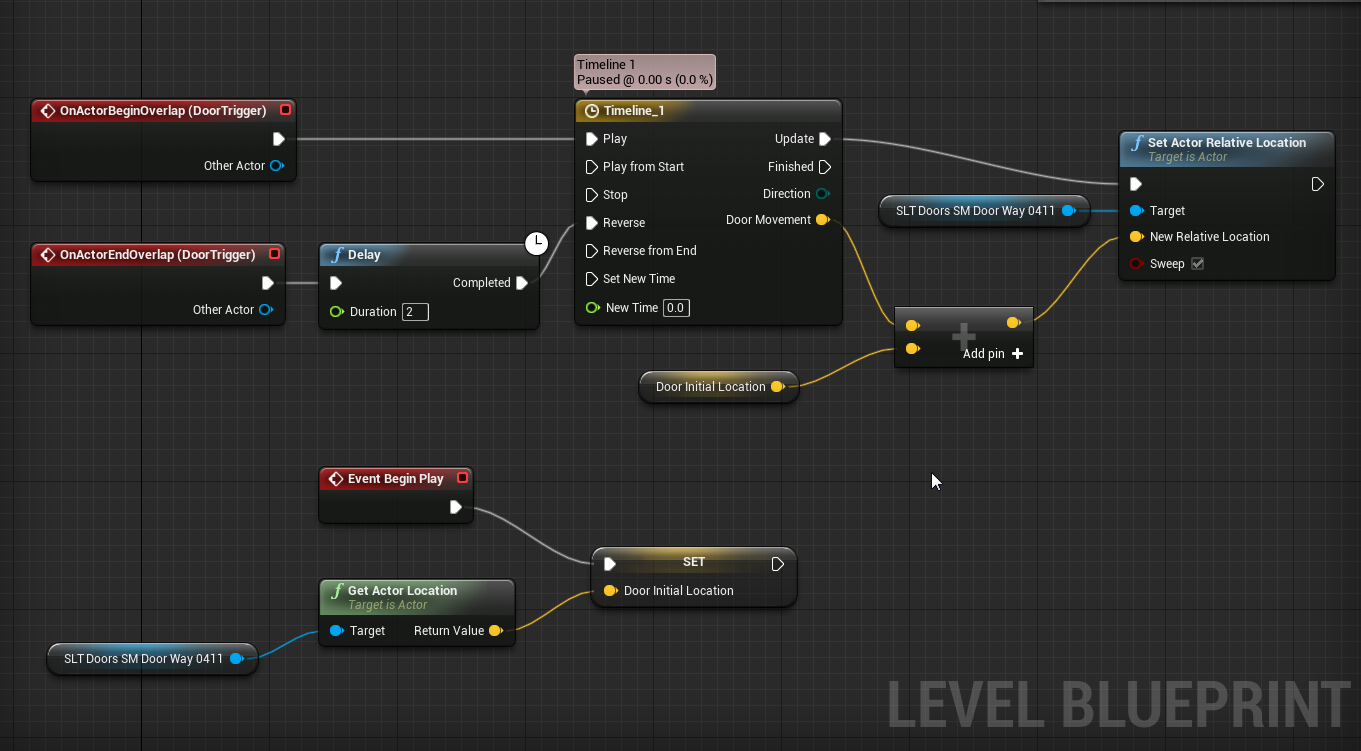
\includegraphics[width=0.5\textwidth]{OtherImages/UEBlueprint.png}
    \caption{Source: \url{https://docs.unrealengine.com/en-US/ProgrammingAndScripting/Blueprints/UserGuide/Timelines/Examples/OpeningDoors/index.html}}    \label{UnrealEngineBlueprint}

\end{figure}

\subsubsection{Unity}
Unity is currently the most commonly used game engine with over 2.5 million registered developers \cite{Unity_arnia_software}. Unity is developed by Unity Technologies and was first released in June 2005.  Over 60\% of augmented- and virtual reality games are created using Unity \cite{GameEngine_UnityGame_book}. 
\\~\\
Unity is free for personal and educational projects. To create the game, Unity allows a lot of features to be used through the GUI, but for full freedom, the creator would need to program in C\#. Unity however provides lots of resources to learn C\#. Unity also combines with Visual Studio where the IntelliSense can help with recommending functions to use as well as spot errors\footnote{\url{https://docs.microsoft.com/en-us/visualstudio/gamedev/unity/get-started/getting-started-with-visual-studio-tools-for-unity}}.


\subsection{Levels of Automation}
When talking about autonomous systems, it is important to know the different levels of autonomy. The modern day Tesla cars are level 3, which means they can be driven autonomously for the majority of the time, but do need a human driver as a fallback system \cite{teslaSelf, Bagloee2016}.
\begin{table}[H]
\begin{tabular}{lll}
\textbf{Level} & \textbf{Name}                   & \textbf{Description} \\
0     & No Automation          & The driver is solely controlling the vehicle\\
1     & Driver Assistance      & Cruise control is an example of this             \\
2     & Partial Automation     & Automatic parking            \\
3     & Conditional Automation & Modern day Tesla cars            \\
4     & High Automation        & Vehicle almost fully automated           \\
5     & Full Automation        & Vehicle never needs human input
\end{tabular}
\caption{Source: \url{https://link.springer.com/article/10.1007/s40534-016-0117-3\#Sec3}}
\end{table}

For this project all our simulations will be level 5. 

\subsection{Mixed Traffic Simulation}
The purpose of a mixed traffic simulation is to model the interaction between different types of agents, for example the the interaction between pedestrians, autonomous robots and vehicles. This is important because having a fully automated agent has to interact with a lot more than only other fully automated agents \cite{KernerBorisS2021Eoad}. 
\\~\\
A mixed traffic simulator can be used to simulate different situations where an autonomous system has to react to other agents behavior. This will mean the implemented algorithm will have the opportunity to try out a lot more complex scenarios a lot faster than in real life. This will help speed up development time. 


\subsection{API}
API stands for Application Programming Interface. This will allow a program to communicate with one-another. The API will define what kind of requests another program can make, how to make them, and the what the format should be. APIs also need to be documented so that other developers know how they work \cite{WulfJochen2020FVCw}.
\\~\\
In the case of our simulators, APIs will be used to communicate between an external program and the simulator itself. These communications could contain information for how to control the agent, or it could contain information from what the agent observes. 

\subsection{Digital Twin}

\subsection{Reinforcement Learning}

\subsection{Imitation Learning}

\subsection{Blender}
%Training machine learning models will be mentioned a few times when looking at the simulators.

\section{Analysis of Existing Simulators} \label{analysisOfSimulators} % \label{BackgroundLit} \label{AoCP}
In this section we will look at a large variety of different simulators, to determine which one best suits our purpose. We will be looking at which operating system and game engine the simulator uses, whether or not it is open source, and the pros and cons of each simulator. We will be particularly looking at the simulators sensing abilities, ability to add additional entities, map customisability, available APIs, and how user-friendly the simulator is. Aspects of the simulator which is not as important as how realistic the simulator physics is, and how visually good looking it is. These are criteria formed by the project specification (Section~\ref{ProjectSpec})
\\~\\
The purpose of this section is to get a good understanding of the different simulators currently in existence.

\subsection{Overview}

% \usepackage{tablefootnote}
% \usepackage{array}
% \usepackage{pdflscape}
% \usepackage{longtable}


% \usepackage{tablefootnote}
% \usepackage{array}
% \usepackage{pdflscape}
% \usepackage{longtable}

\begin{landscape}
% \usepackage{tablefootnote}
% \usepackage{array}
% \usepackage{rotating}
\begin{table}
\resizebox{\columnwidth}{!}{%
\begin{tabular}{lllllllllll}
\textbf{Simulator~ ~ ~ ~ ~} & \textbf{\thead[l]{Open\\Source}} & \textbf{OS}\tablefootnote{"Any" means most commonly used Linux distributions, Windows and MAC} & \textbf{Game Engine} & \textbf{Development}\tablefootnote{"Actively Developed" means that there were several releases in the past year} & \textbf{Support} & \textbf{Pedestrians} & \textbf{Extensibility} & \textbf{\thead[l]{Multiple\\Agents}} & \textbf{Existing APIs} & \textbf{\thead[l]{Worth\\Considering}\tablefootnote{Reasoning for the decision can be found in the Appendix \ref{Appendix}}} \\
4DV-Sim & No & Linux & \thead[l]{PhysX\\(Physics Engine)} & \thead[l]{Actively\\ Developed} & Company offers support & Yes & No & Yes & Yes & No \\
AirSim & Yes & Any & \thead[l]{Primarily UE4,\\ but also Unity} & \thead[l]{Actively\\ Developed} & GitHub Issues & No & Yes & Yes\tablefootnote{Multiple agents is possible, but in a very limited number and has to be declared at the start.} & Yes & Yes \\
Apollo & Yes & Docker & Unity & \thead[l]{Actively\\ Developed} & GitHub Issues & No & Difficult & No & No & No \\
Autoware & Yes & ROS & N/A & \thead[l]{Actively\\ Developed} & GitLab Issues & No & Difficult & No & Limited\tablefootnote{\label{Footnote:03_Background:SimulatorResearchLimited}No sensing APIs} & No \\
Carla & Yes & Linux\tablefootnote{Linux is the main platform and they are aiming to support Windows as well. Currently Carla does not work on Windows.} & UE4 & \thead[l]{Actively\\ Developed} & GitHub Issues & Yes & Yes & Yes & Yes & Yes \\
CoppeliaSim & Yes\tablefootnote{More information can be found here: \url{https://www.coppeliarobotics.com/helpFiles/en/licensing.htm}} & Any & \thead[l]{Several different \\ physics engines} & \thead[l]{Actively\\ Developed} & Forum\tablefootnote{\url{https://forum.coppeliarobotics.com/}} & Yes & Difficult & Yes & Yes & No \\
CrowdSim3D & No & Any & N/A & Unknown & Company offers support & Yes & No & Yes & Yes & No \\
Deep Drive & Yes & Any & UE4 & \thead[l]{Last Commit\\ June 2020} & GitHub Issues & No & Yes & Yes & No & No \\
\thead[l]{Donkey Car\\ Simulator} & Yes & Any & Unity & \thead[l]{Actively\\ Developed} & GitHub Issues & No & Yes & No & Limited\footref{Footnote:03_Background:SimulatorResearchLimited} & No \\
Gazebo & Yes & Any & \thead[l]{Several different \\ physics engines} & \thead[l]{Actively\\ Developed} & GitHub Issues & Yes & Yes & Yes & Yes & Yes \\
LPZRobots & Yes & Linux & \thead[l]{ODE\\(Physics Engine)} & \thead[l]{Last Commit\\ November 2018} & Google Group\tablefootnote{\url{https://groups.google.com/d/forum/lpzrobots}} & Yes & Yes & Yes & No & No \\
\thead[l]{LGSVL\\ Simulator} & Yes & Windows 10 & \thead[l]{Several, both \\ Unity and UE4} & \thead[l]{Actively\\ Developed} & GitHub Issues & Yes & Difficult & Yes & Yes & Yes \\
Marilou & No & \thead[l]{Linux and,\\ Windows} & N/A & \thead[l]{Latest release\\ was 2018} & Non & Yes & No & Yes & No & No \\
rFpro & No & Windows & ISIMotor & \thead[l]{Actively\\ Developed} & Company offers support & No & No & Yes & No & No \\
Rig of Rods & Yes & \thead[l]{Linux and,\\ Windows} & \thead[l]{Creates its own \\ soft-body physics engine} & \thead[l]{Actively\\ Developed} & Forum\tablefootnote{\url{https://forum.rigsofrods.org/}} & No & Yes & Yes & No & No \\
TORCS & Yes & \thead[l]{Linux and,\\ Windows} & \thead[l]{Non, implemented \\ from scratch} & \thead[l]{Latest release\\ was 2016} & Discussion page\tablefootnote{\url{https://sourceforge.net/p/torcs/discussion/11281/}} & No & Yes & Yes & No & No \\
Webots & Yes & Any & \thead[l]{ODE\\(Physics Engine)} & \thead[l]{Actively\\ Developed} & GitHub Issues & Yes & Yes & Yes & Limited\tablefootnote{Only sensing APIs} & Yes
\end{tabular}%
}
\caption{The table contains a brief overview over some of the simulators researched. \\ For more detailed information on the simulators see Appendix~\ref{}.}
\end{table}
\end{landscape}

\subsection{Further Simulator Analysis}
Compare the different simulators that were interesting from the previous table.

\subsection{Conclusion}
Explain which simulator to go for
% In this section, we will look at which of the three simulators to use from Section~\ref{BackgroundLit}.%, as well as 

% \subsection{AirSim vs Carla vs Gazebo}
% For this section, I started off building the different simulators from source. The aim was to build the simulators in Ubuntu, but due to my outdated graphics card, I was unable to build Unreal Engine. I was however able to run Unreal Engine on Windows by downloading the binary distribution. 
% \\~\\
% \textbf{AirSim:} The AirSim plugin built successfully on Windows\footnote{\url{https://microsoft.github.io/AirSim/build_windows}}, and I was able to use it in Unreal Engine. The only minor inconvenience was that the simulator has to be built using the Visual Studio 2019 development terminal. However, after installing Visual Studio 2017 which is used to build Carla, I was no longer able to build AirSim. 
% \\~\\
% As AirSim is built using a game engine, it would hopefully mean it is an easier environment to set up missing features. AirSim is also designed to simulate traffic, unlike Gazebo which is designed for a variety of simulations. 
% \\~\\
% \textbf{Carla:} Carla built successfully on Ubuntu following this guide\footnote{\url{https://carla.readthedocs.io/en/latest/build_linux}} and after doing these alterations:
% \begin{itemize}
%     \item As I was using Ubuntu 20.04 I had to install Python2/Pip2 using curl
% \item Clang-8 was outdated so I installed Clang
% \item Clang-Tools-8 was outdated so I installed Clang-Tools
% \item lld-8 was outdated so I installed lld
% \end{itemize}
% However, as Unreal Engine did not build on Ubuntu I was unable to proceed from here and instead tried on Windows. Carla claims to work on Windows, but I ran into a build error which I was unable to resolve. This seems to be a known issue, and as of the time of writing, is still an unresolved issue on GitHub\footnote{\url{https://github.com/carla-simulator/carla/issues/3605}}. 
% \\~\\
% Another issue with Carla was the ability to import custom maps \cite{Carlamap}. Carla requires the map to consist of two layers. The first one being the map structure with buildings and roads, whilst the second one will consist of road rules, such as traffic lights, where the cars are allowed to drive, pedestrian crossings, and so on. RoadRunner\footnote{\url{https://uk.mathworks.com/products/roadrunner.html}} can be used to import maps, but this is not a free product.
% \\~\\
% \textbf{Gazebo:} Gazebo built successfully on Ubuntu\footnote{\url{http://gazebosim.org/tutorials?tut=install_ubuntu&cat=install}}.
% \\~\\
% Gazebo has all the sensing features we are looking for \cite{Rosique2019}, such as GPS, LiDAR, RADAR, and Ultrasonic. One main drawback with Gazebo is the lack of existing APIs to interact with multiple entities at once. Even though the Gazebo platform has a lot of features, it is not as rich as Unreal Engine \cite{EbeidEmad2018AsoO}. 
% \\~\\

% \textbf{Conclusion:} As we are not able to build Carla, as well as it being very difficult to change maps, we will discard that one and look at comparing AirSim and Gazebo. 
% \begin{itemize}
%     \item AirSim and Unreal Engine is more feature-rich than Gazebo. Using Unreal Engine will also minimise chances of finding out something is not possible later on.
%     \item Both have the ability to import maps quite easily
%     \item Both have the ability to train machine learning models.
%     \item AirSim has GPS and Lidar, but it is not clear if it has Ultrasonic or not. Gazebo has more sensing APIs in any case.
%     \item Having multiple entities seems easier in AirSim than in Gazebo. 
%     \item AirSim is designed for vehicles, whilst Gazebo is designed to be a more generic robotics platform. 
%     \item Gazebo is more commonly used than AirSim. 
% \end{itemize}
% After looking at the information above we have chosen to go with AirSim for this project. This is because AirSim is a plugin for Unreal Engine and that gives us the option to extend the program to anything Unreal Engine allows us to do. 

%%%%%%%%%%%%%%%%% Requirements Capture
\chapter{Requirements Capture} \label{ReqCap}
The objective of this project is to create a simulation environment where mixed forms of traffic can interact with one another. The simulator should be able to be flexible in its use cases and have a large variety of features. It is also very important that the simulator is easy and intuitive to use.  

The main goal is to have a good base platform on which users can conduct experiments. The users should have the flexibility of adding custom models and environments to the simulator. These steps must be straightforward. The project should also demonstrate how this can be done by looking at several alternatives. 

The system should also contain some machine learning models of mixed traffic interaction. This is used both to illustrate how this can be achieved, but also to show the complexity of the system. 

\section{Simulator Requirements}\label{simRequirements}
The project should look at existing simulators and \textbf{compare} them against the following criteria.
\begin{itemize}
    \item \emph{Usability:} The simulator should be simple to set up and use.
    \item \emph{Extensibility:} The simulator must be extendable. This means adding new features and modifying existing features should be possible. 
    \item \emph{OS:} The simulator should run on Ubuntu.
    \item \emph{Game Engine:} The game engine is the core component of a simulator. Using an outdated game engine could make future work challenging. Simulators with no game engines could be hard to understand and debug. 
    \item \emph{Development:} The simulators would ideally be actively developed. This minimises the chances of running into issues later on with outdated libraries. 
    \item \emph{Support:} If issues cannot be resolved having community support could be vital.
\end{itemize}
\\~\\
\paragraph{}The simulator should have the \textbf{following features}:
\begin{itemize}
    \item \emph{Multiple Agents:} Having the simulator handle multiple agents is crucial to perform mixed traffic simulation. It does not however need to handle large crowds.  
    \item \emph{Variety of Agents:} Adding new models and behaviour to the simulator should be a simple process. This should include pedestrians. 
    \item \emph{Free movement:} The agents should be able to move freely around the environment. This means that they should not be restricted using any external rules. 
    \item \emph{Customisable environments:} It should be straightforward to change the simulation environment. 
    \item \emph{Controlling APIs:} It should be possible to control the agents from external programs. The control should include simple navigation, but also the ability to add and delete entities. 
    \item \emph{Perception APIs:} These could include cameras or LIDARS. Perception APIs would be APIs that could give the user the ability to obtain an understanding of the agents' surrounding. 
\end{itemize}


\section{Environment requirements}
This section will list the requirements decided for the environment:
\begin{itemize}
\item \emph{Real location:} It would be preferable to be able to replicate real locations. 
\item \emph{Outdoors:} The environment should primarily be outdoors.
\item \emph{Simplicity:} To create the environment should not be a challenging task. Importing the model into the simulator is down to the simulator itself, but the environment should be of a format that makes this easy. 
\item \emph{Customisable:} The process of creating the maps should allow the user to modify the maps if needed. 
\end{itemize}

\section{Deliverables}
The main deliverables for this project will be:
\begin{itemize}
    \item An analysis of available simulators with a conclusion for which one would be best to use for the project.
    \item A flexible simulator that has the ability to easily add additional models and simulate mixed traffic.
    \item A simulator with the incorporated sensing and controlling APIs.
\item Scripts to demonstrate the features available to the simulator. 
\item Documentation explaining how to use the APIs.
\end{itemize}





%%%%%%%%%%%%%%%%% Analysis and Design
\chapter{Analysis and Design} \label{design}
This chapter provides a high-level overview of the core components of the AirSim architecture. The chapter will look at how the simulator has been adapted for this project, the design decisions made, and the limitations. 

As the project is extending an existing code-base, the design decisions aimed to limit the impact on the existing structure. This was to allow future updates to the master project, to benefit this one as well. Most of the changes to this project were made in Unity, but changes were also made in AirLib and the wrapper to allow for additional APIs. 

\section{AirSim Functional Overview} \label{05:Overview}
Figure~\ref{ADA:Figure:OriginalOverview} shows a simplified overview of the important components in the original AirSim architecture. It is key to understand each of these components, as they are all updated throughout the project. 


The project consists of 4 main components, Unity, which is written in C\# and contains most of the simulator logic, AirLib which is written in C++ and contains the server, the AirLib Wrapper which is written in C++ and acts as a bridge between AirLib and Unity, then finally the code where the user can interact with AirLib through the APIs. As this project is very modular, it gives the user the freedom and flexibility to choose a game engine and input language. 

This section will contain a brief overview of each of the 4 components. This is to better understand the design decisions made in Section~\ref{05:ArchitecturalDesign}. Figure~\ref{05:stringList} shows an example of how the user interaction layer can interact with Unity. 

\begin{figure}[h]
    \centering
    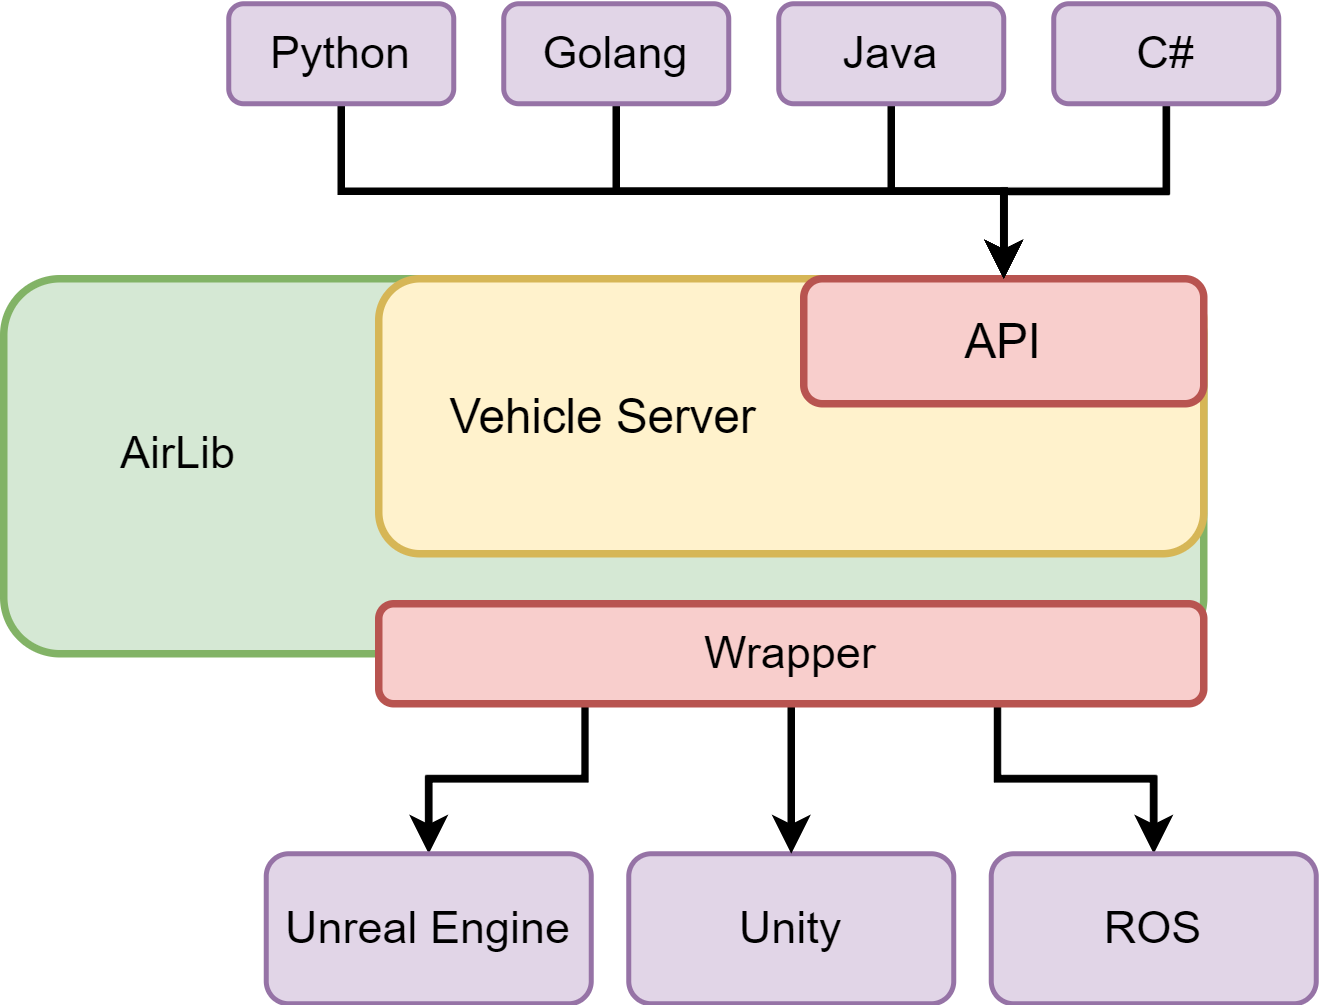
\includegraphics[width=0.5\textwidth]{05_AnalysisAndDesign/Diagrams/OriginalOverview.png}
    \caption{High-level overview of the core components of AirSim used for this project. Only one server exists and all API calls are passed to it.}
    \label{ADA:Figure:OriginalOverview}
\end{figure}

\begin{figure}[h]
    \centering
    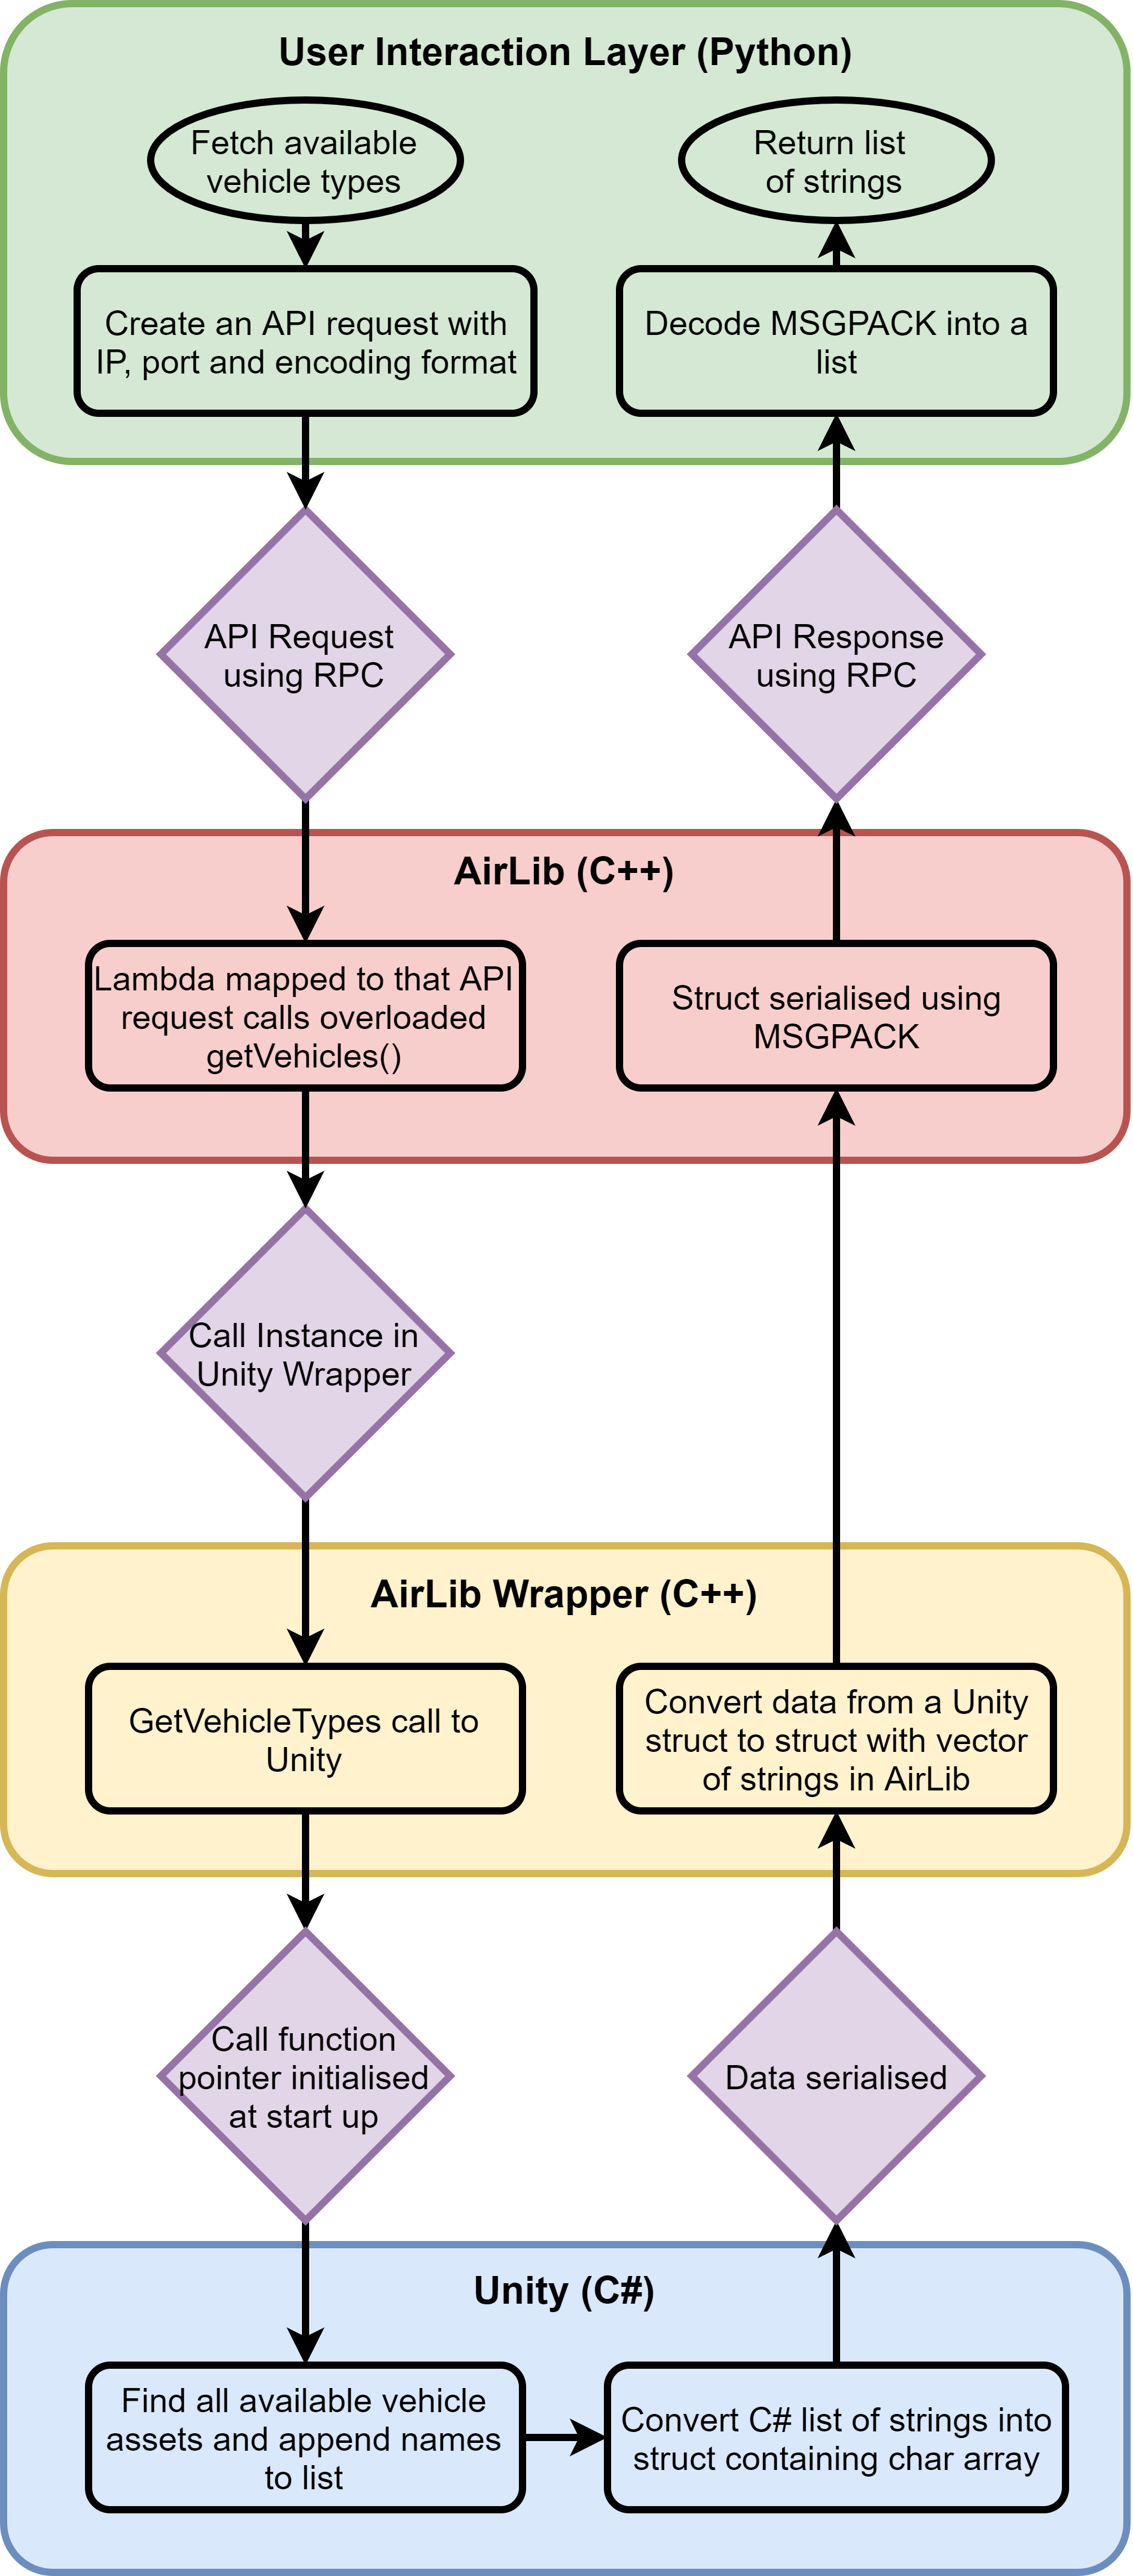
\includegraphics[width=0.6\textwidth]{05_AnalysisAndDesign/Diagrams/stringArray.png}
    \caption{High-level overview of the API that fetches available vehicle types. For APIs that require arguments, these will be encoded and added to the API request. The main change between different API requests is what happens in Unity.} \label{05:stringList}
\end{figure}

\subsection{AirLib} \label{05:AirLib}
AirLib is the main component of AirSim and where the majority of the code is located \cite{}. This self-contained library consists of four main components. The first one is a physics engine. This component is lightweight and designed to be simple to add new vehicles and drones. The next component is a sensor model. This component contains header-only models for external sensors such as GPS and Barometer. The third component is the vehicle module. Currently, the only model implemented is for PX4 QuadRotor\footnote{\url{https://docs.px4.io/master/en/getting\_started/}}, which is a platform that can be used to control drones. The last component is the control library. This part provides abstract classes for the APIs and implementations for specific platforms. 

This project does not use the physics engine, sensors module and vehicle modules in AirLib. The project is instead using the Unity version of these components. Instead, this project focuses almost solely on extending the control library. On startup, AirLib creates AirLib creates a server using RPCLib\footnote{\url{https://github.com/rpclib/rpclib}} which can interact with the APIs over a TCP channel. The advantage of using RPC is that it allows for a range of different programs as well as being fast and lossless (Section~\ref{05:UIL}). The design decision to move the physics engine and sensors to Unity is further discussed in Section~\ref{05:ArchitecturalDesign}. 

\subsection{AirLib Wrapper}
A wrapper is used for AirLib to communicate with Unity. Using a wrapper allows for a variety of different game engines as well as other physical systems such as ROS. This makes AirSim more modular, which again can increase the extensibility of the program. The wrapper will implement the interfaces declared in the vehicle module (Section~\ref{05:AirLib}). At startup, Unity will pass function pointers to the wrapper so that later the APIs can call those functions. The wrapper will also create an instance of AirLib which will set up the RPC server. The wrapper also handles the conversion of the data from C\# to C++.

\begin{figure}[h]
    \centering
    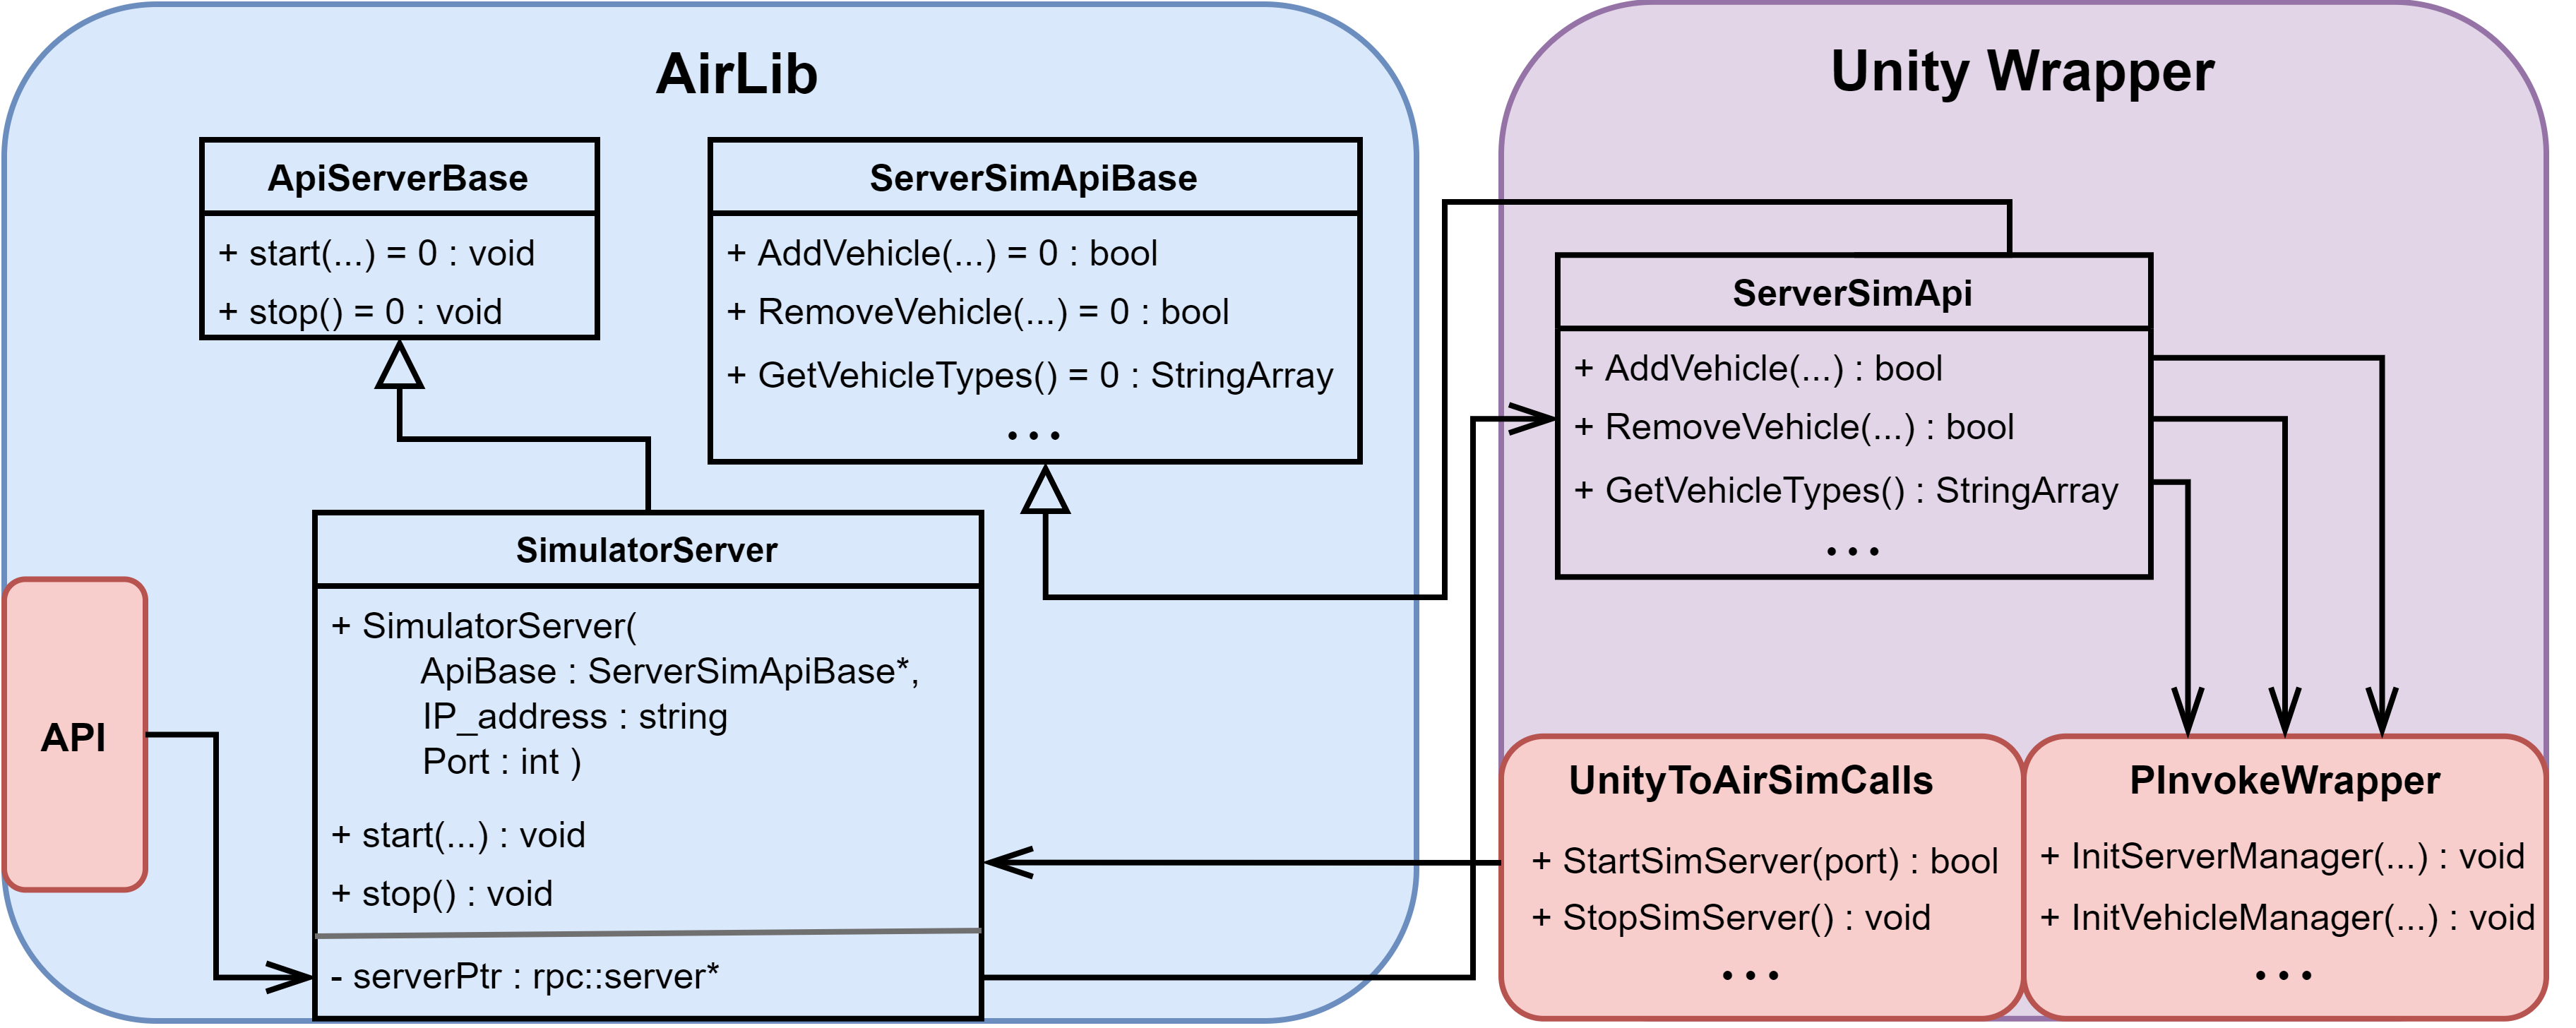
\includegraphics[width=1\textwidth]{05_AnalysisAndDesign/Diagrams/UnityWrapper2.png}
    \caption{A simplified view of how AirLib and the Unity Wrapper link together. UnityToAirSimCalls and PInvokeWrapper are red boxes to illustrate that they are only files containing functions. The other objects are classes. The black arrows show examples of functions calls. The details of how Unity starts the server is left out in this diagram.} \label{05:fig:UnityWrapper}
\end{figure}

Figure \ref{05:fig:UnityWrapper} shows an example of how AirLib links to the Unity Wrapper. AirLib has an interface for the available APIs that are then overridden in the wrapper. These overridden member functions will then access the function pointers initialised at startup by Unity. This is done by having Unity call the InitServerManager with the arguments being the function pointers. As was explained in Section~\ref{05:AirLib}, the API interacts with the server initialised at startup. In this case, the server is stored in the SimulatorServer class and will call functions overridden from the ServerSimApiBase class. Unity can also make calls to the wrapper at runtime. These are done through the UnityToAirSimCalls. The figure shows a slightly simplified for how Unity can start and stop the server. To create the server, the wrapper creates a new instance of the ApiServerBase and initialises it with a pointer to the ServerSimApi. It is clear from this figure that another game engine can easily be used by changing the overridden functions. 


\subsection{AirSim with Unity}
As will be discussed in Section~\ref{05:AD:UEvUnity}, Unity was chosen as the game engine for this project. Unity works as the physics engine and all of the simulator logic is solely done in Unity. One of the disadvantages of using Unity is that it is not thread-safe. This means that the AirSim plugin has to interact with the simulation through shared memory. This will be explained further in the implementation section (Section~\ref{06:airsim}). All of the simulator logic is solely done in Unity.

AirSim works as a plugin for Unity. AirLib and the wrapper are compiled into a single DLL file which can be interacted with through Unity. This allows the user to use all the features in Unity when creating maps and environments. This also makes it easy to set up an AirSim environment as only the DLL and a setup object has to be added to the scene.  


\subsection{User Interaction Layer} \label{05:UIL}
AirSim allows for a variety of different languages to interact with AirLib. This is because the API calls use MessagePack\footnote{\url{https://msgpack.org/}} also known as MsgPack. MsgPack allows for an efficient binary serialisation\footnote{\url{https://github.com/msgpack/msgpack/blob/master/spec.md}}. MessagePack supports over 50 programming languages and environments. These include C\#, Golang, Haskell and others.  For this project, only Python will be used. This is because Python is a flexible language that makes prototyping quick and easy. The existing code for the user interaction layer is already written in Python, so it will be more beneficial to continue with this rather than starting from scratch.

In the Python project, three classes are implementing the APIs for each of the servers. This is to make it clear which type of entity the user is communicating with. It also avoids confusion when passing controls to the simulator, as pedestrian and vehicles use different controls. Python allows for external tools like OpenCV to process the images passed from the Simulator. Figure~\ref{} shows a diffusion map generated by OpenCV using two images created by forward-facing cameras on a car. The diffusion map highlights objects that are shifted more between the two images, i.e. the object has to be closer. 


\section{Architectural Design and Limitations} \label{05:ArchitecturalDesign}
This section will look at some of the architectural decisions made when modifying the existing AirSim design. The section will also look at what limitations were introduced by these decisions. Section~\ref{06:airsim} will go into more detail about how the design decisions were implemented. 


\subsection{Unreal Engine or Unity} \label{05:AD:UEvUnity}
After AirSim was chosen as the simulator, the main decision to be made was which game engine to use. AirSim primarily uses Unreal Engine, but there is also a prototype version using Unity. As mentioned in the background section (Section~\ref{GameEngines}), Unreal Engine has better graphics than Unity. Using Unreal Engine would also mean that the simulator more complete with many more features available such as dynamic weather, more sensors and more APIs. Generally, Unreal Engine also has better performance than Unity\cite{vsmid2017comparison}. The disadvantage of using Unreal Engine is that it makes it harder to rapidly prototype and add new features. This is because the existing code is much more complex. It is also because Unreal Engine is not as simple to use as Unity. In Unity, the simulator can run in debug mode making it possible to update scripts whilst the program is running. This is not possible in Unreal Engine where a small change can take a couple of minutes to compile. 

There are several advantages to using Unity over Unreal Engine. Firstly, Unity's asset store provides a large range of plugins and models that can be used. The key ones that are of interest for this project are the UMA models (Unity Multipurpose Avatar), which can be added to model pedestrians, and the ML-Agents tool kit, which can be used to train reinforcement learning models. Both of these addons will be explained further in the implementation section (Section~\ref{06:airsim}). The second advantage of using Unity is the simplicity of having scripts. This makes debugging simpler as the scripts can be interacted with at runtime. The scripts can also be attached to objects which makes it easy to create several instances of an entity. Another advantage is that as using Unity as the game engine is currently only an experimental version, only the most important features have been implemented. This makes the existing code easier to navigate than the code written for Unreal Engine. This can also be seen as a disadvantage of using Unity. As only a few APIs have been implemented, a lot of work has to be put in to have the same features available in Unity as currently are available in Unreal Engine\footnote{\url{https://microsoft.github.io/AirSim/unity_api_support.html}}. 

Overall using Unity for this project would be more beneficial than using Unreal Engine. Unity allows for rapid prototyping which is more important for this project. Unity's ML-Agent also makes it easier to train reinforcement models for the part of the autonomous system of this project. 

\subsection{Moving logic to Unity}
Section~\ref{05:AirLib} explained how AirLib is split into four parts and that this project would only focus on the vehicle module. AirSim is designed in such a way that software components are easily exchangeable. As can be seen from Figure~\ref{ADA:Figure:OriginalOverview}, ROS, which is a robot operation system, could be used instead of a game engine. AirSim would then be able to model the behaviour of the real robot without needing the game engine. As this project would only focus on the simulation, this was not a feature that was needed. Instead, it was easier to move all the physics calculation to Unity along with other logic such as controlling the vehicles. Making this design decision would make it much easier when adding the pedestrians. Currently, the physics engine in Unity would need a redesign to get something like autonomous wheelchairs and pedestrians to work.

The consequence of this is that the simulation behaviour could differ between the different game engines. AirSim would also not work for pedestrians without the Unity game engine. As this project is only a prototype, the simplification of moving the logic to Unity will still be beneficial. 

% Modularity
\subsection{Dividing the server} \label{05:dividingServer}
The decision to split the server in AirLib was the main change to the existing design of AirSim. This design change was needed for several reasons. Firstly, how the server is implemented currently, all API calls are single-threaded, which means that one call has to be processed before the next one is handled. This makes the API that captures images slow as it has to wait for one game tick before returning the image. (See Figure~\ref{06:imageCapture} in Section~\ref{06:airsim}). Another reason for doing this was to simplify the code structure. As can be seen from Firgure~\ref{05:SplitServer}, dividing the AirLib server to handle the game state, vehicles and pedestrians separately was a natural split, especially as the pedestrians would introduce a large number of new APIs. This split would make it clear which entity is being controlled and which APIs are available. Also, in the current design, the server only exists if there is a vehicle in the scene. If the vehicle is removed, the server is closed. This also means that there has to be a vehicle in the scene to start the server.  This is not the desired behaviour as a user would want to be able to spawn in and delete both vehicles and pedestrians at any time. 

\begin{figure}[h]
    \centering
    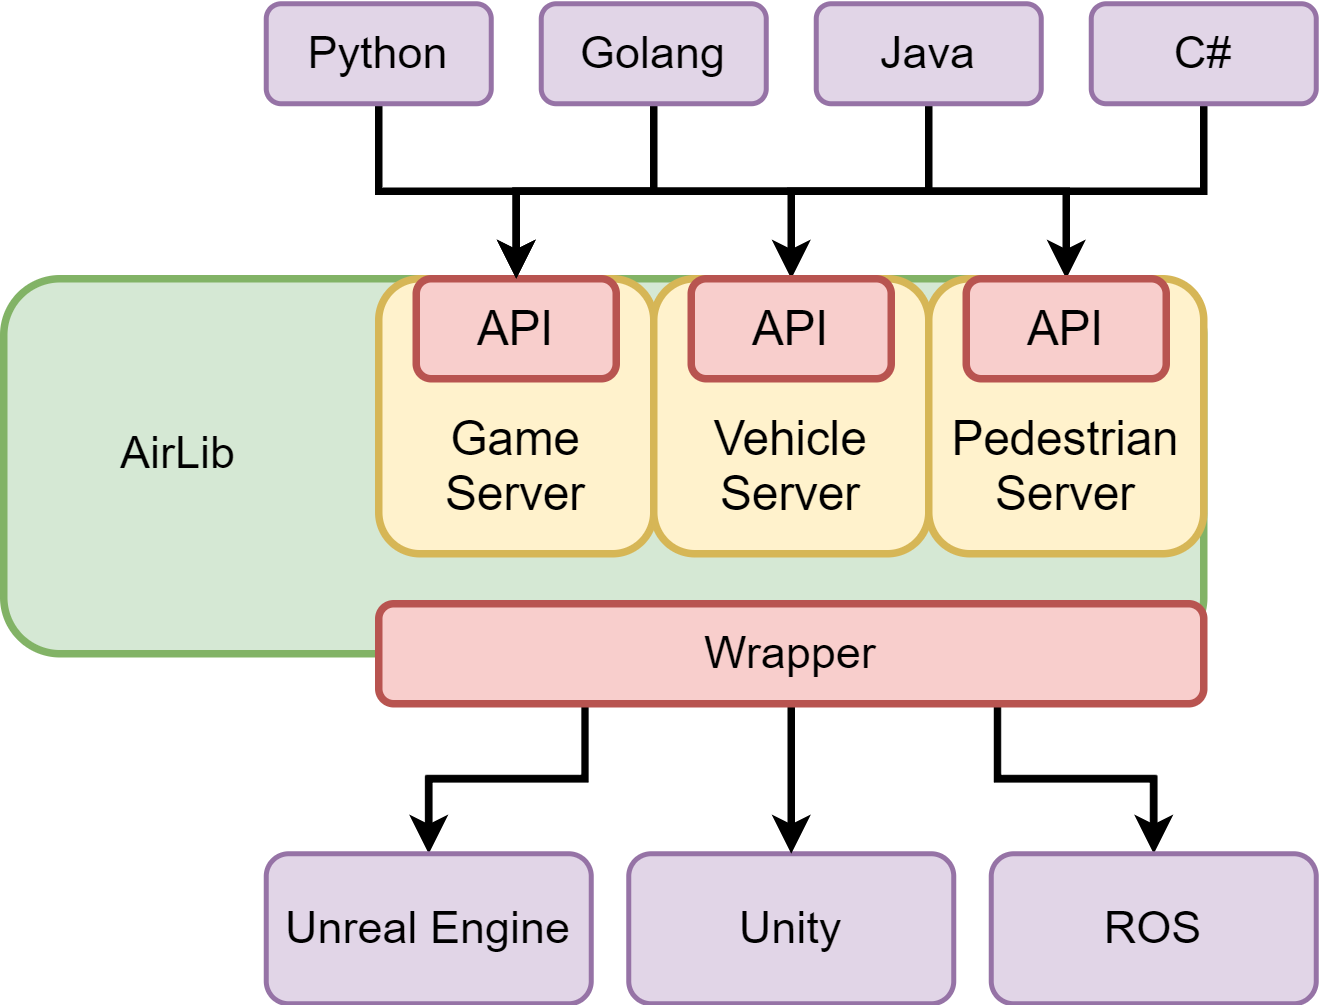
\includegraphics[width=0.5\textwidth]{05_AnalysisAndDesign/Diagrams/UpdatedOverview.png}
    \caption{Separate APIs into several servers on different ports. This makes it easier to expand the APIs and add additional features.}\label{05:SplitServer}
\end{figure}

The division was done by replicating a simplified version of the server creation and then moving the APIs for the game state over to this one. As mentioned in the functional overview (Section~\ref{05:Overview}) AirLib has a lot of features that this project does not need. When replicating the server initialisation, these parts were left out. In Unity, the code was changed in such a way that at startup, the game server will start, and the user can communicate with the server, such as printing, spawning and deleting vehicles and pedestrians, and so on. When the first vehicle is spawned the server vehicle server will start, and when the last is deleted, the server will close. This behaviour is the same for the pedestrians. 

This project benefits in several ways when dividing the server. Firstly, as mentioned above, the server would now start running at startup. This means that users can control the game state without vehicles having to be in the scene. Secondly, dividing the APIs makes the code more readable. Originally it is difficult to see if an API call acts on the server or the vehicle. Another benefit of the split is that the game server can communicate instantly with the server instead of having to wait for the other calls to the vehicle server to finish. Finally, with the current implementation, it would be easy to open up a separate server for every vehicle. This could be beneficial as separate scripts could run a specific vehicle. This change is now possible as the code is designed in such a way that it can start a new server on request. 

However, there are several limitations and disadvantages to this new approach. Firstly, if too many servers are launched the overhead will be too big and the performance would decrease. Currently, this is not an issue with only three servers, but with one server per entity, this could be slow. Secondly, if for example, a developer wants to use different means of communication for the APIs, rather than RPC, this would require several changes in multiple files. Finally, as this is a major change to the existing AirSim, pulling new features from the master repository will no longer be straightforward. 

Overall the benefits still outweigh the disadvantages. As having multiple entities in the scene at once is a key part of this project, separating the APIs relating to the game from the APIs relating to the vehicle allows for this. This also works as a proof of concept if performance becomes an issue and a server per entity becomes needed. 


%Why was this needed.
% •	Server was only single threaded
% •	This meant slow especially when getting images
% •	Pedestrian controls were different. Make it easier to distinguish between the two.
% •	Separate server controlling APIs
% •	Limit the number of API calls going to one serverS
% How was this done
% •	Extract Server APIs from the existing vehicle server
% •	Create Pedestrian API server from scratch. 
% How does it improve things	
% •	Makes it more readable as everything is not in one big class.
% •	Makes it possible to control pedestrians and vehicles from different scripts
% •	A simple modification can be made to set up even more servers, for example one per entity.
% •	If multiple servers was created they would still communicate in the same way with Unity, so every instance could still talk to every entity. 
% •	Simulator at startup
% What does it break/limitations
% •	If for example wanted to use different communications means than RPC, this would require changes in several files. 
% •	In some ways not as easy to navigate as all the code is not in one place. 
% •	Increased server overhead. (Not much for 3, but if there were over 100 this could be a problem. 
% •	As this is a major change to AirLib, future updates to AirSim will not be incorporated automatically. 


%\subsection{Simplifications}
%\section{Architectural Limitations}




%%%%%%%%%%%%%%%%% Implementation
\chapter{Implementation} \label{implementation}
\section{Expansion of AirSim}
This section will cover which features were modified and added to AirSim to reach the desired behaviour. Each section will look at the challenges faced and discuss previous approaches. The sections will also explain which bits of existing code the feature is based off, or if the feature was written from scratch.

\subsection{Requirements}


\subsection{Multiple Entities}
The first modification to be made to the simulator was to make sure that it could handle multiple agents. This was an essential step as the simulator could not be used if having several agents at once was not possible. Currently, the simulator is primarily designed for one agent. After initial research, the simulator should have been able to handle two vehicles if this was added to the startup configuration. However, this did not work in Unity. 

The first step was to modify the existing APIs so that the vehicles could be accessed individually. To do this, all vehicles were added to a global list. Each vehicle was also given a unique identifying name. The next step was to add an argument to each API specifying the vehicle.  When a vehicle API was called, Unity would first iterate over the map looking for the corresponding vehicle. Once the entity was found Unity would then forward the API request to that vehicle. This change had to be made throughout AirSim tracing the call from the user interaction in Python to Unity. 

The main challenges faced when doing this was originally trying to adapt the configuration file. As this had not been properly implemented in Unity yet, time was spent trying to debug this issue. Eventually, it was discovered that adding the vehicles manually to the scene before starting would be easier. 

Currently, if two vehicles are given the same name the second vehicle will spawn, but the API calls will only be redirected to the first vehicle. This can easily be changed so that either both entities should behave in the same way, or that the second entity does not spawn. This behaviour however was seen as unimportant and have been left out for the time being. 
 

\subsection{Spawning Entities at Runtime}



% \begin{figure}[h]
%     \centering
%     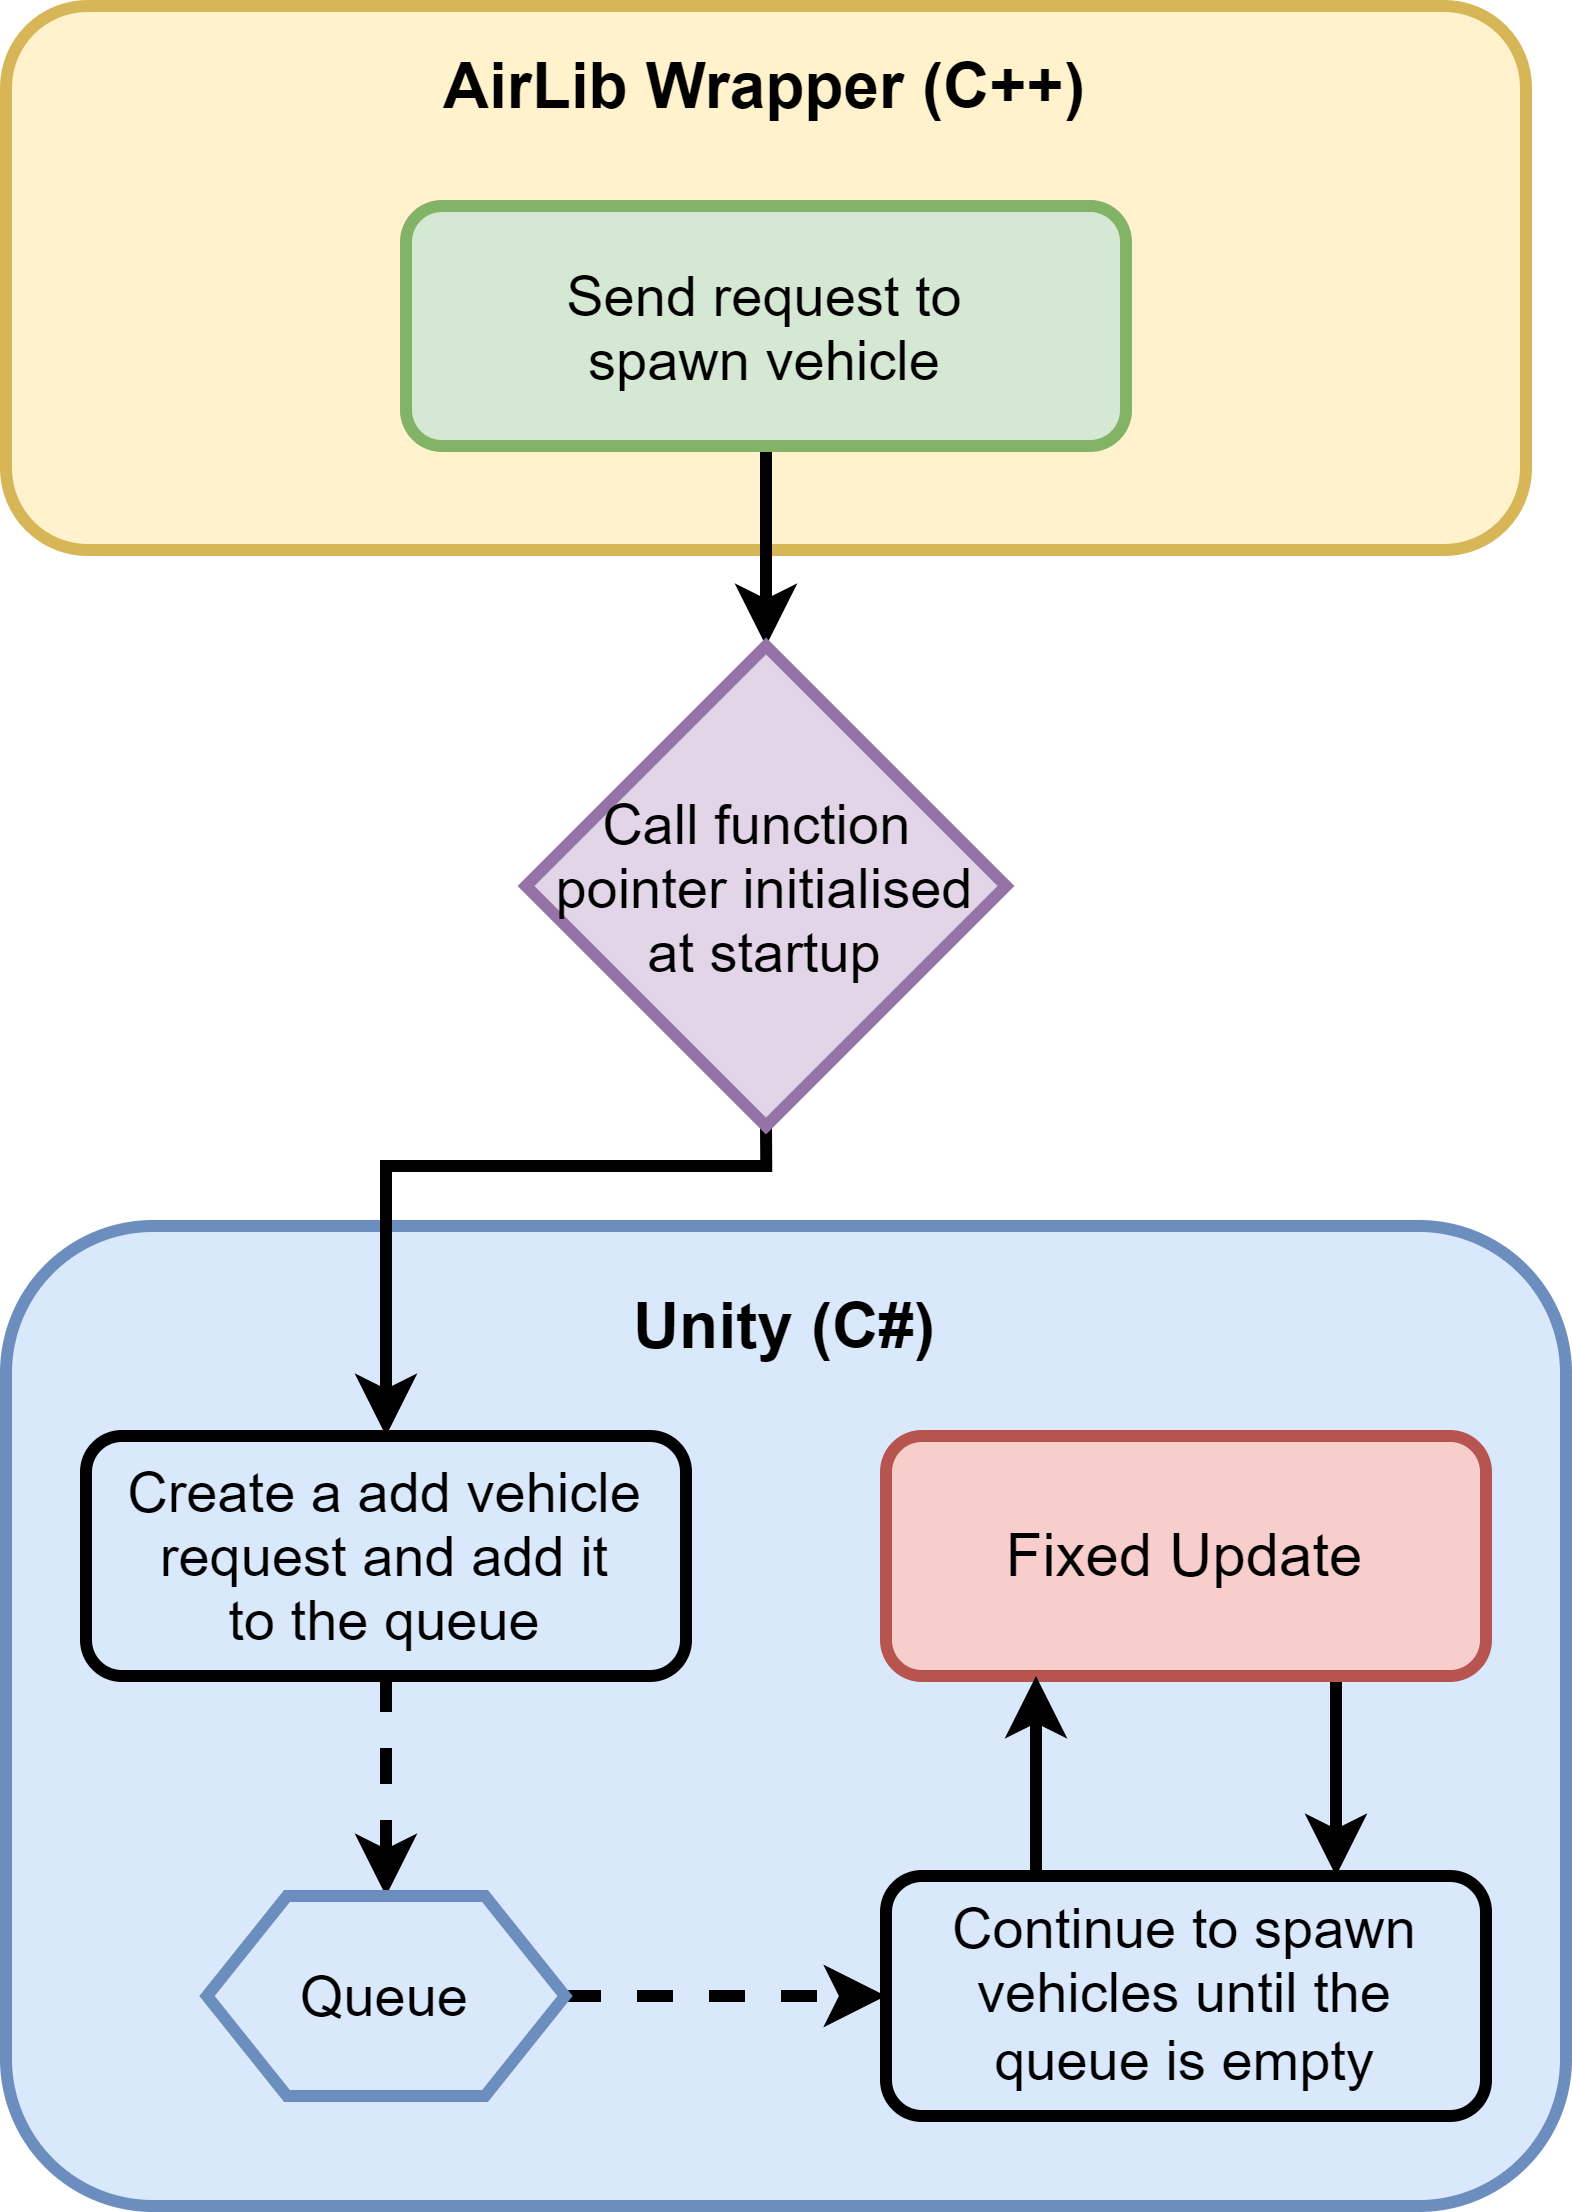
\includegraphics[width=0.5\textwidth]{06_Implementation/00_AirSim/Diagrams/spawnVehicle.png}
%     \caption{Unity is not thread-safe, so the server has to interact with the simulator through shared memory.} \label{06:spawnVehicle}
% \end{figure}


Being able to spawn entities at runtime was a desired feature as it would allow the users to have full control of the simulation through the APIs. This was not an existing feature as the simulator was not designed to simulate several entities at once. As mentioned in the section above, multiple vehicles could be declared in the configuration file. This file however is only loaded at the start and never reloaded whilst the simulator is running. 

\begin{wrapfigure}{r}{0.5\textwidth}
    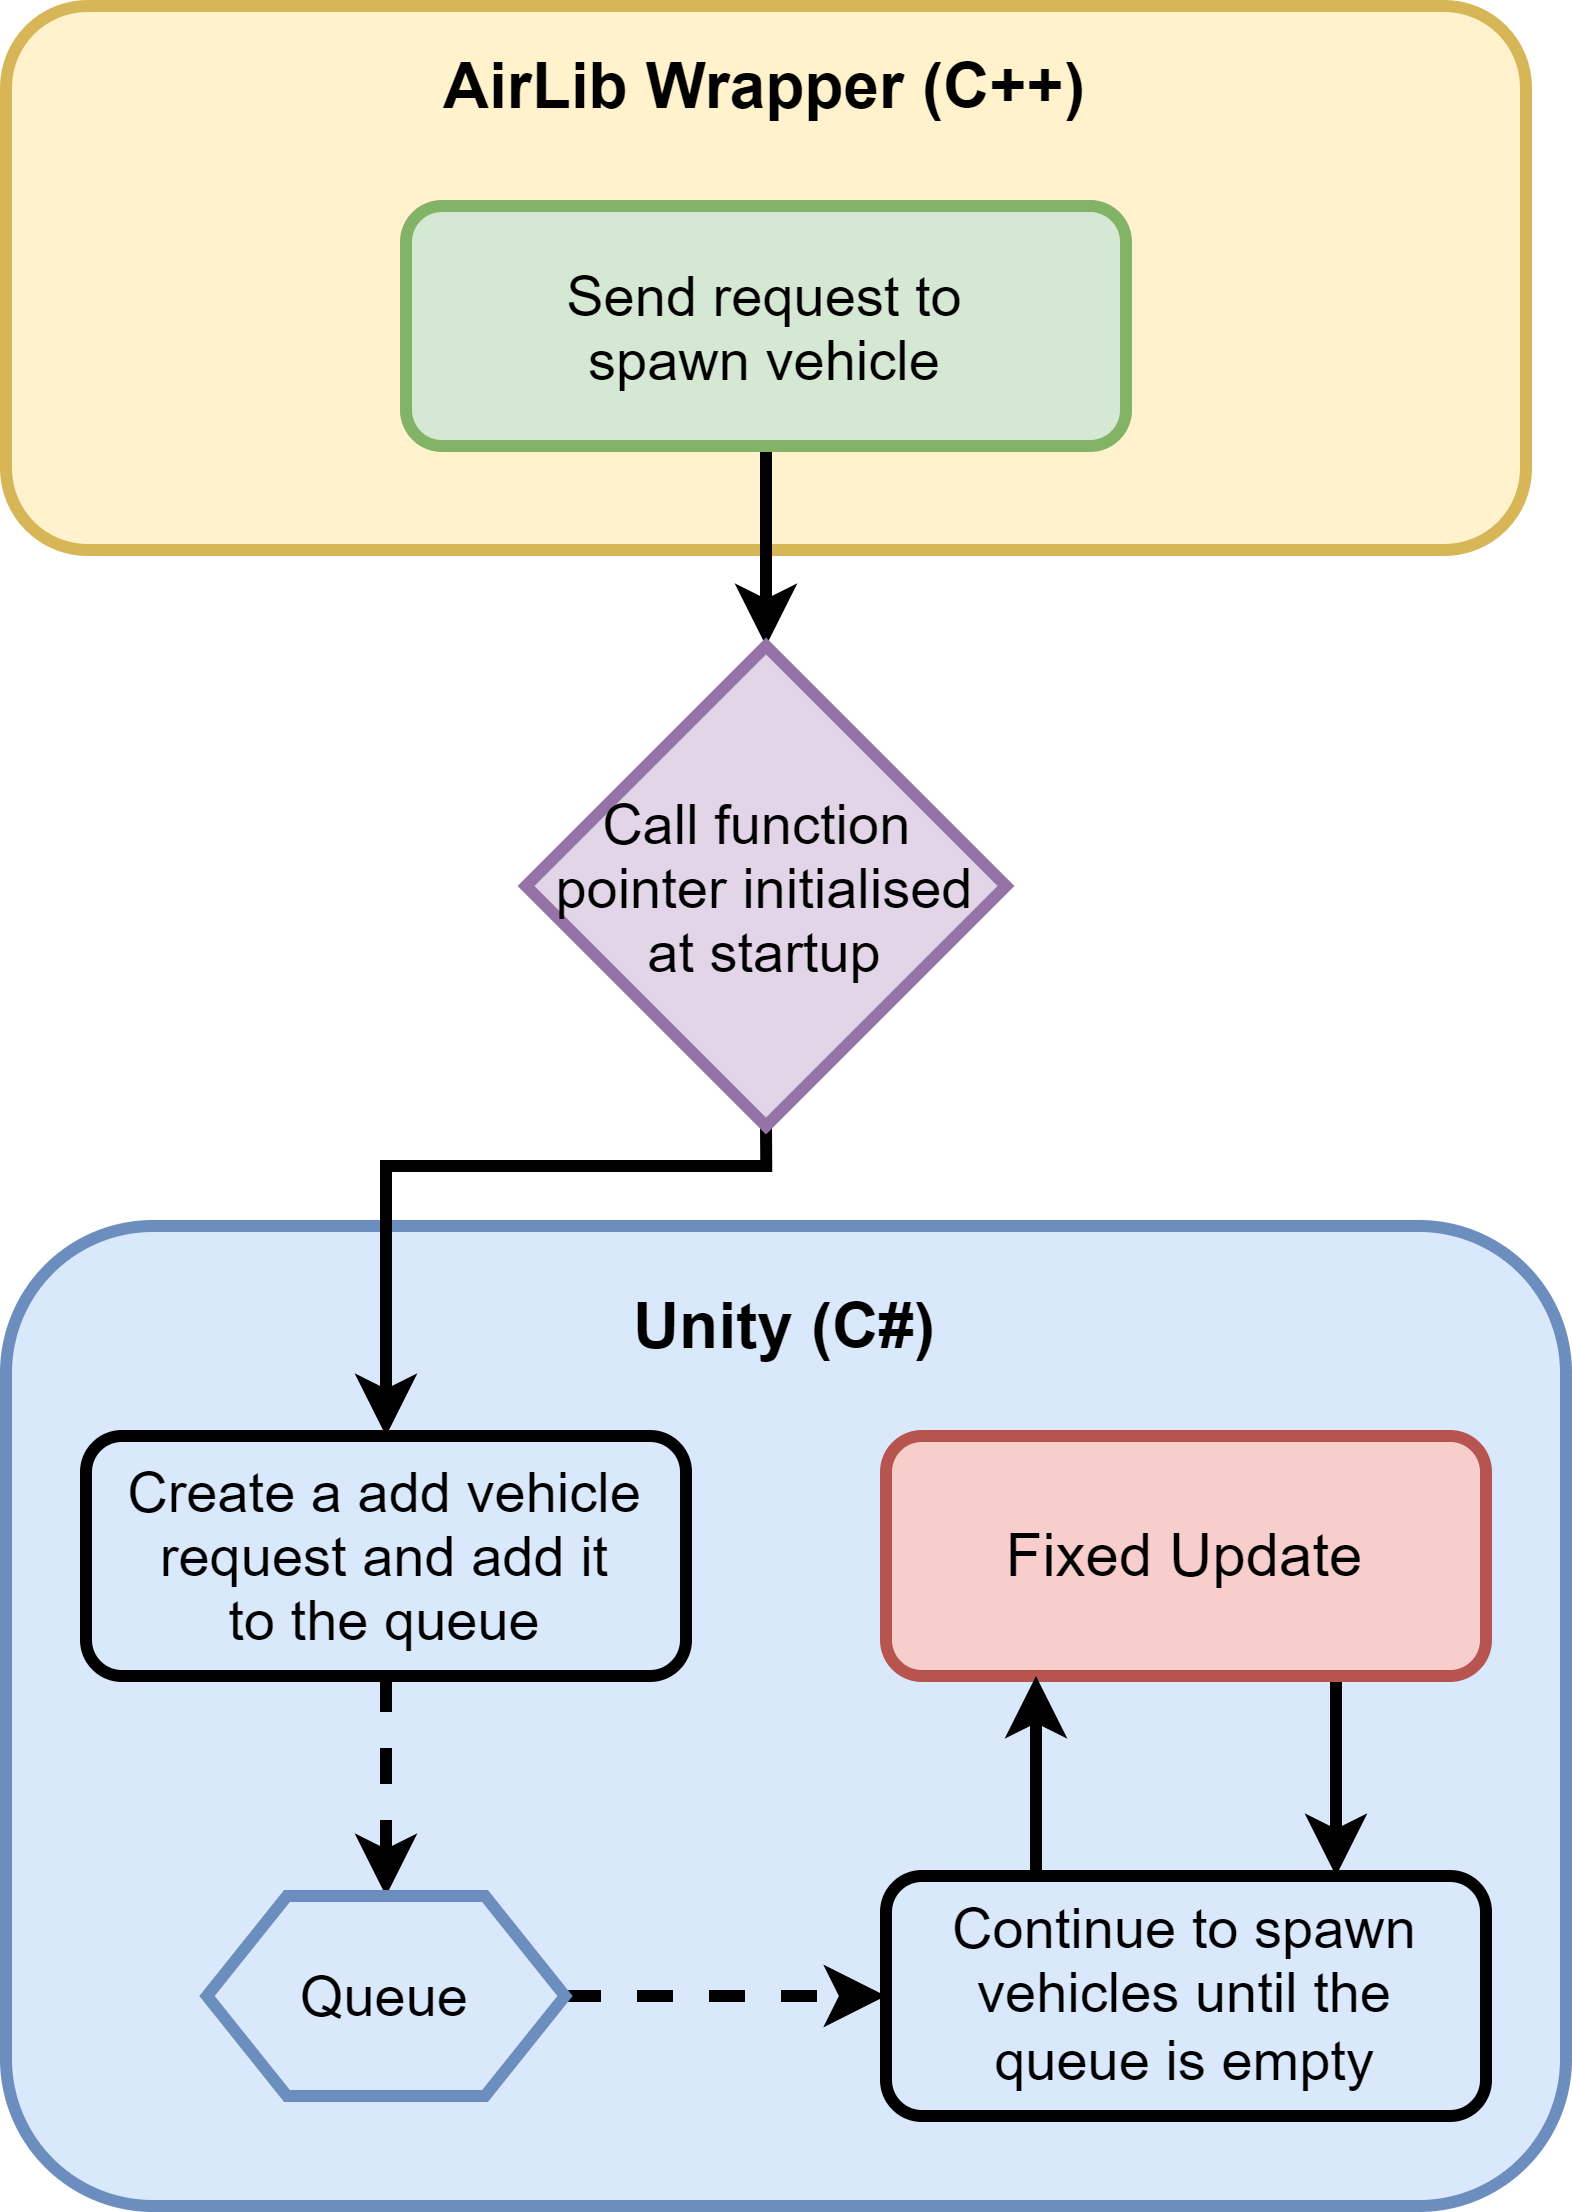
\includegraphics[width=0.5\textwidth]{06_Implementation/00_AirSim/Diagrams/spawnVehicle.png}
    \caption{Unity is not thread-safe, so the server has to interact with the simulator through shared memory. For simplicity, the figure ignores everything that happens before the wrapper.} \label{06:spawnVehicle}
\end{wrapfigure}

The first change that had to be made to AirSim was to add the new API. The API would take in four arguments: the vehicle type, the identifying name, the spawn coordinates and the initial rotation. The first issue that had to be resolved was that Unity is not thread-safe. This means that the server could not directly interact with the simulator behaviour. As can be observed from Figure~\ref{06:spawnVehicle}, this was resolved by creating a request which was added to a queue. The fixed update cycle would then check if this queue was empty on every game tick. This means that the user can quickly send several requests to the server and they all get spawned within a few game ticks of each other. 

Another change that had to be made was when the server was instantiated. In the original implementation, the server was connected to the vehicle itself. This meant that the server was only running when there was a vehicle in the scene. To fix this a server object was added to the game scene. The server would now open when the server started, and close when the simulator stopped. (See Figure~\ref{A:MonobehaviorFlow} in the Appendix). Moving the server to a separate game object caused a few issues with the action order. However, these were fixed by moving the vehicle initialisation to the awake stage. Pedestrians would use the same structure once added. 

The alternative to spawning the entities at runtime is to have an object pool, where all of the entities can wait until needed. However, this is not needed as the vehicles are fast to load. For more complex entities this could be a better option. The disadvantage of using this method is that there will then be a limit to the number of entities as users cannot generate more if they run out. 


\subsection{Video feed} \label{06:VideoFeed}
One of the requirements for this project was to have sensing APIs (Section~\ref{}). With the Unity game engine, AirSim can return a captured frame to the user interaction layer. The return is a struct that consists of the camera settings, image type, image width and height and the binary image data. This is then converted back into an image in Python. This API had to be updated as the frames rate returned by the server was low, especially when introducing more vehicles. 

\begin{figure}[p]
    \centering
    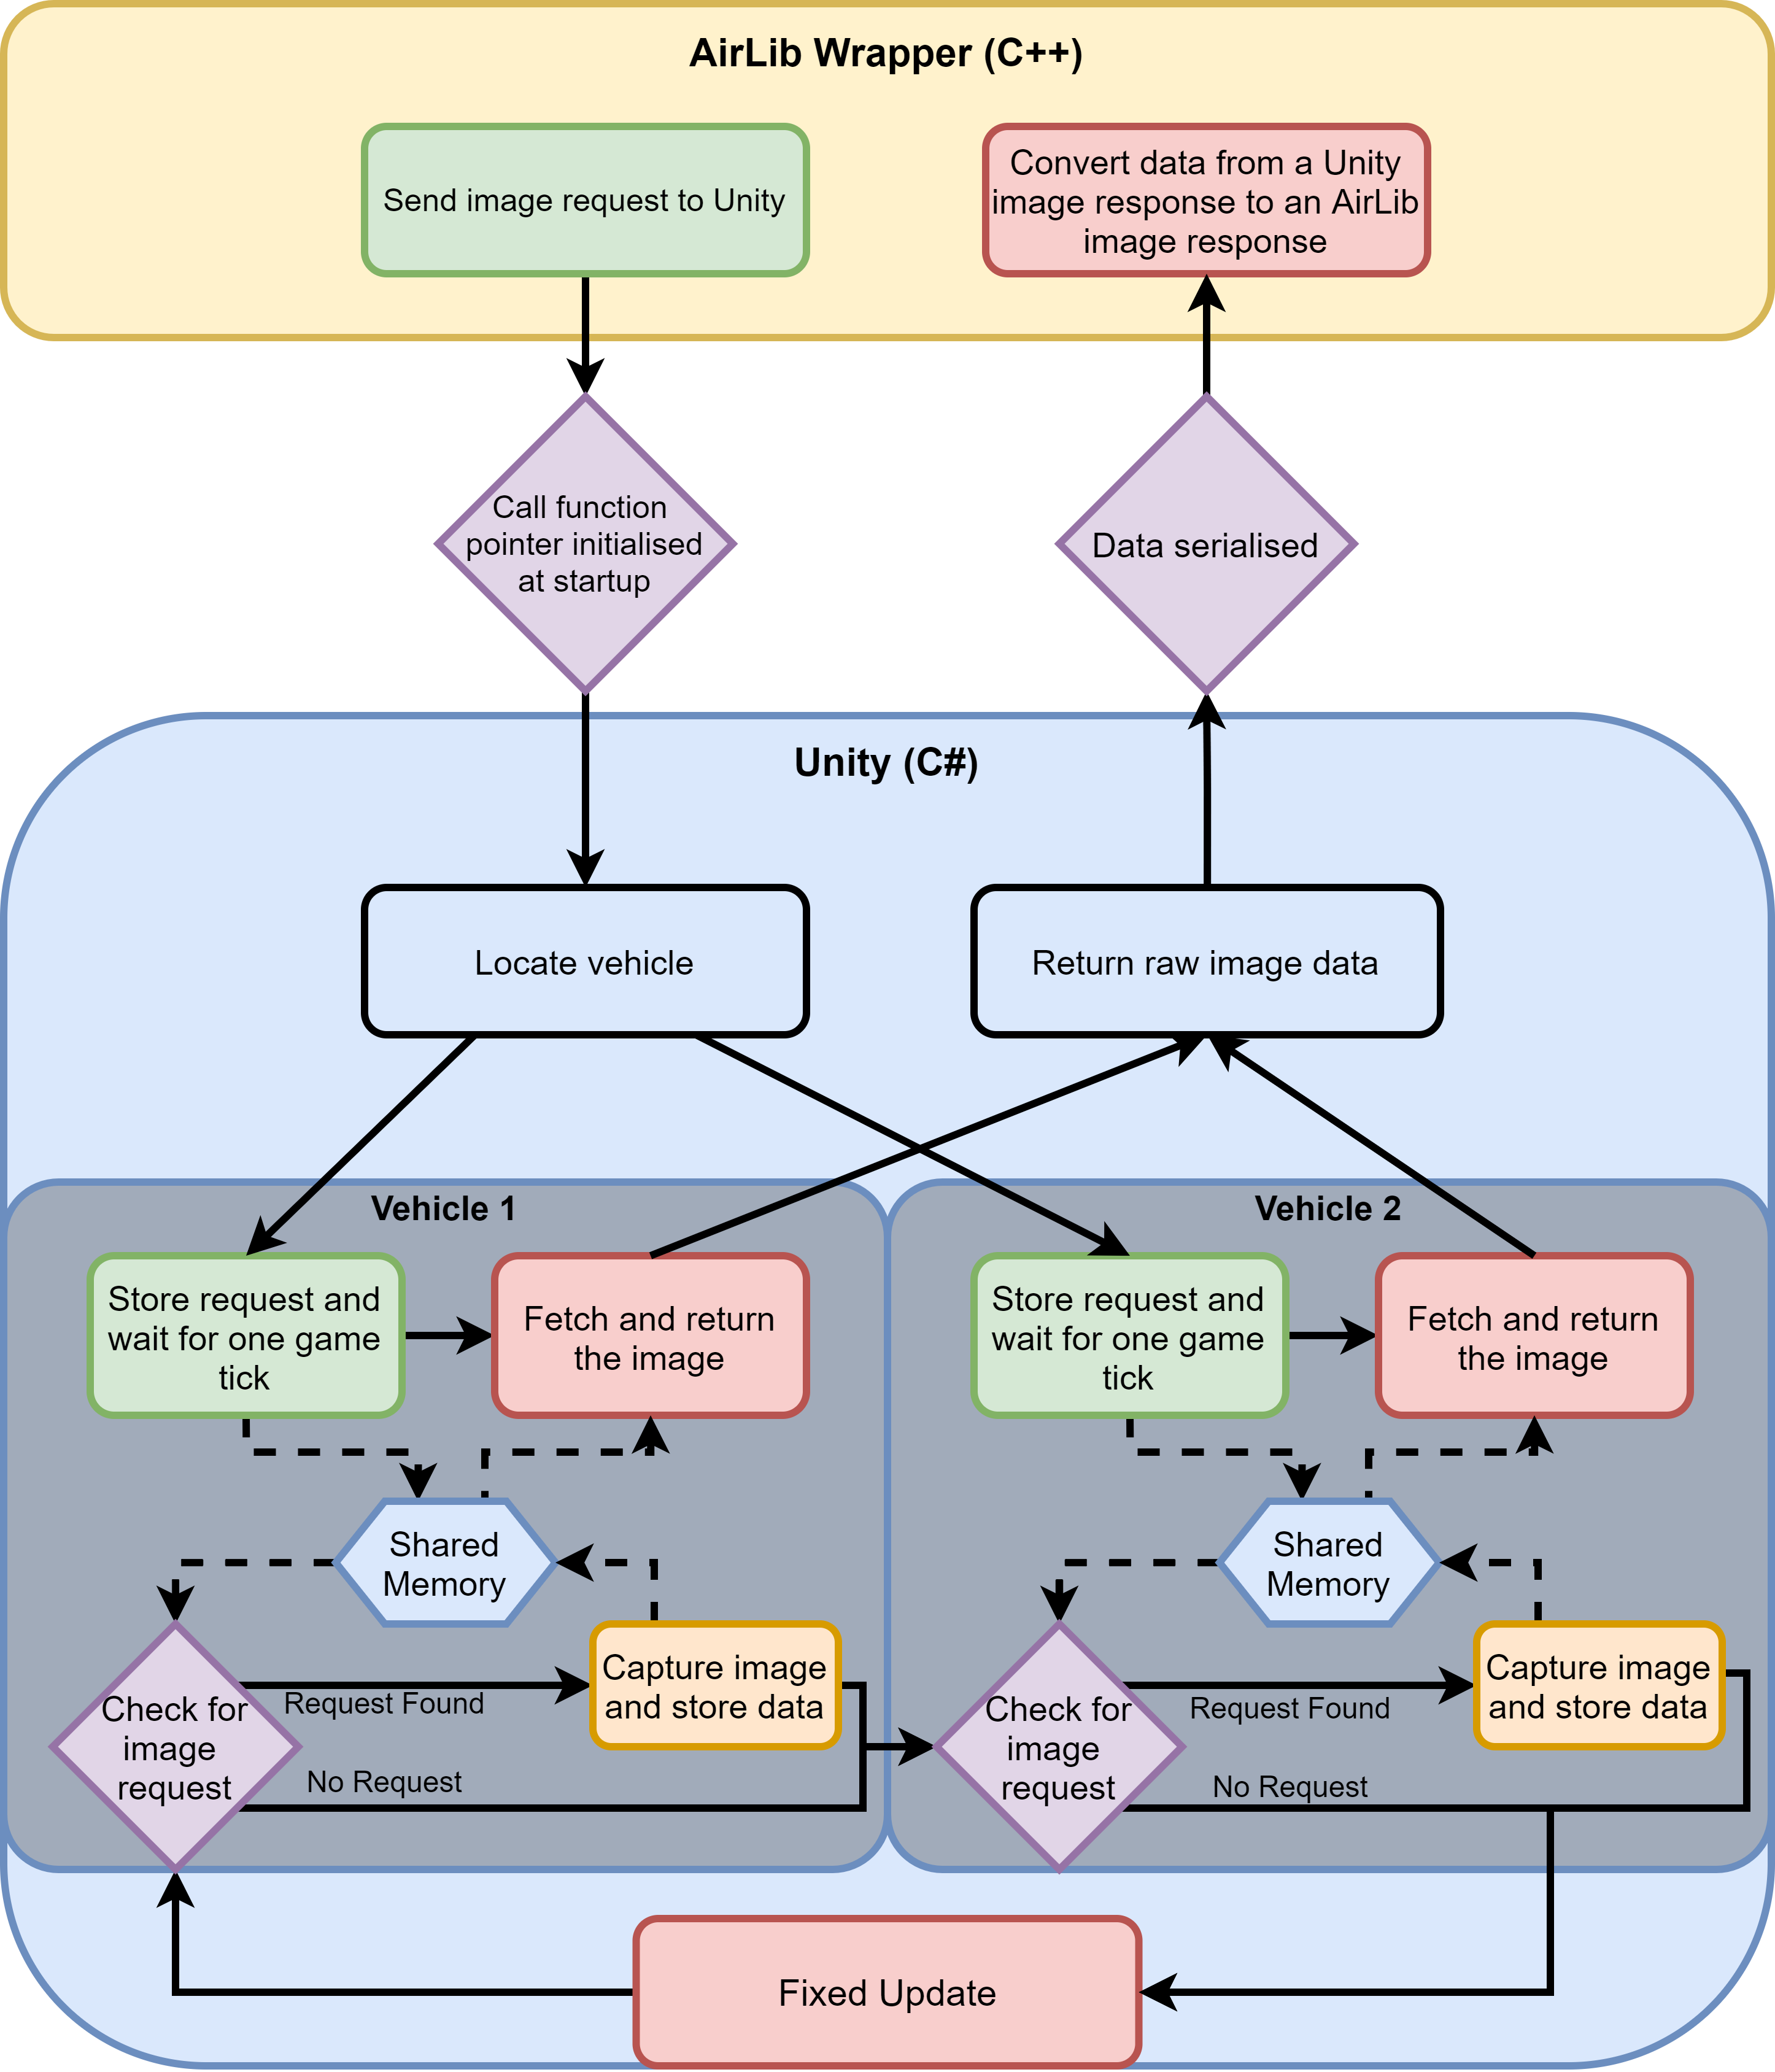
\includegraphics[width=1.0\textwidth]{06_Implementation/00_AirSim/Diagrams/imagecapture.png}
    \caption{} \label{06:imageCapture}
\end{figure}

Figure~\ref{06:imageCapture} shows the existing implementation of how the fetch image API works. Note, only the AirLib wrapper and Unity components are displayed in the diagram. The first part is to pass the image request to the correct vehicle. The image request contains the camera name and type. Unity supports different image types such as scene, which renders the textures as usual, depth and infrared. The call then waits for one game tick and then returns the image response. As can be seen, this method has little impact on the simulator performance as capturing one image does not take long. However, the issue arises when several image requests are happening at once. As the server is single-threaded, the first request has to return before the next one is processed. Using coroutines in Python does not resolve this issue either as the requests will just be queued. One option is to open several servers as mentioned in Subsection~\ref{05:dividingServer}. This however can produce a large overhead when there are many entities. The simulator is running at 120 game ticks per second.

Up to 5 cameras, this method works well. Assuming the calls happen one after the other and a capture takes one game tick, all 5 cameras can return an image in 5 ticks. This means that the frame rate is 24 frames per second. However, two vehicles would half that to 12 FPS, and so on. The output frame rate would therefore be $120/(n*c)$ where n is the number of vehicles and c is the number of cameras per vehicle. The advantage of this method is that it does not impact the tick rate of the simulator. 

\begin{wrapfigure}{r}{0.7\textwidth}
    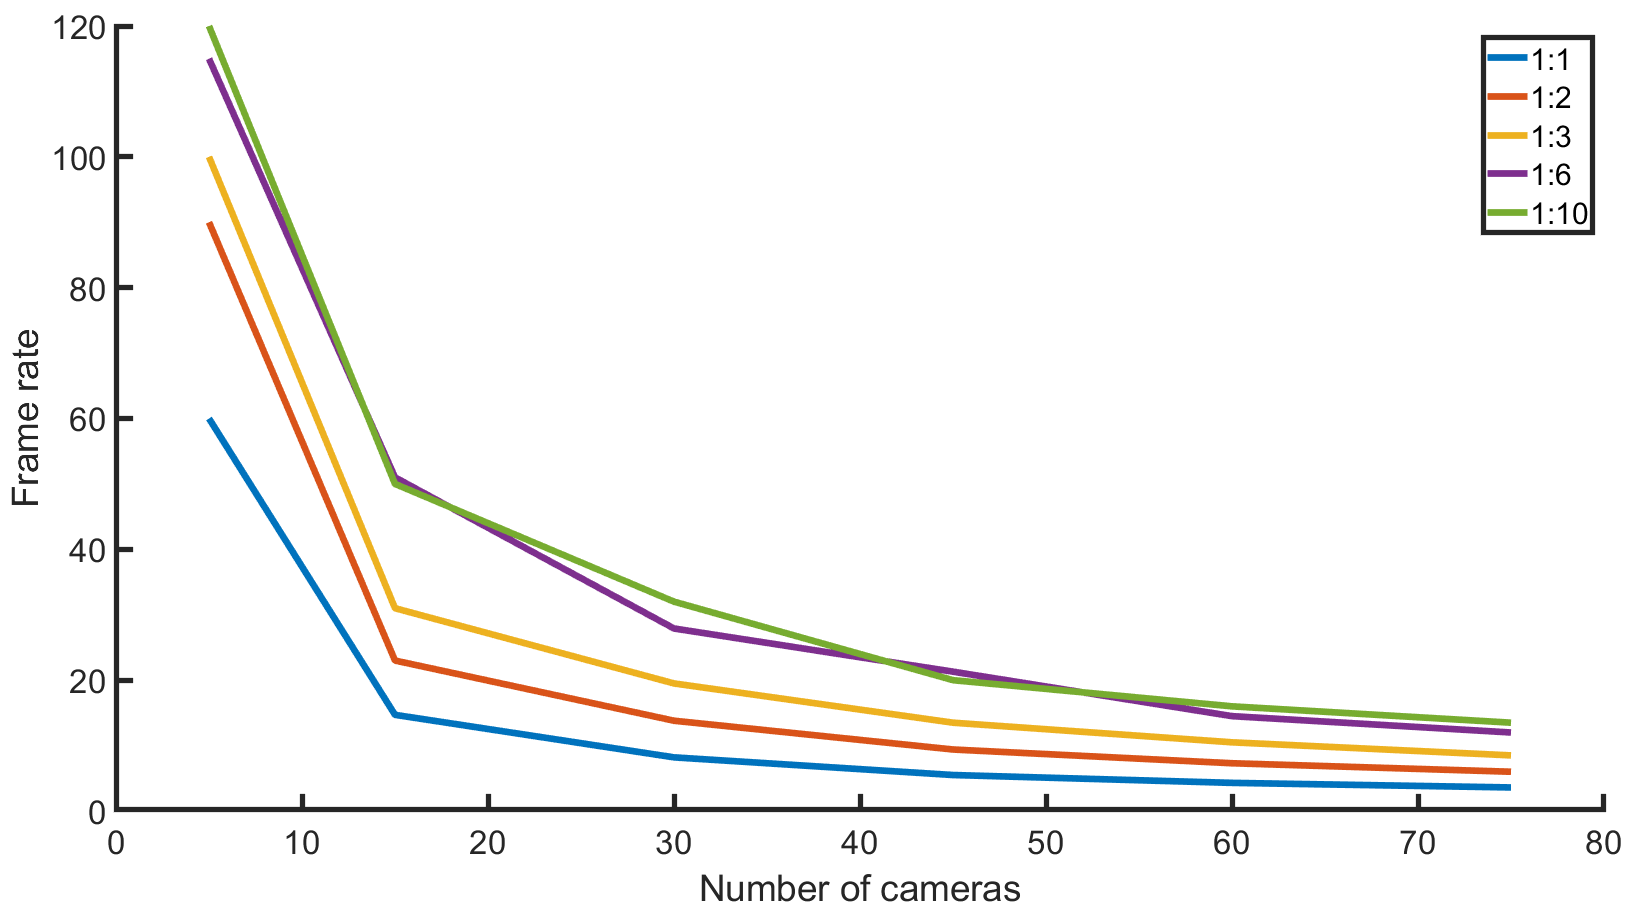
\includegraphics[width=0.7\textwidth]{06_Implementation/00_AirSim/Diagrams/frameRates.png}
    \caption{As the number of cameras are added to the scene the simulator frame rate decreases. By not rendering every camera on every frame the simulator frame rate increases. Each line represents a ratio for how often the camera renders, i.e. 1:2 means the camera frame is rendered every other game update.} \label{06:frameRates}
\end{wrapfigure}
The following changes aim to increase the output frame rate and optimise the APIs so that calls take less time, whilst trying to limit the impact on the simulator tick rate. 

When the vehicle starts, all attached cameras are loaded into a list. Instead of waiting for a request, the images are continually streamed to the server. This is illustrated in Figure~\ref{06:imageCaptureUpdated}. The user can enable and disable cameras to optimise the process. Every enabled camera stores the captured image in the server mapped to the vehicle and camera name. The figure shows how the API request does not have to interact directly with Unity, but can instead fetch the image directly from the server. This change means the server can request several hundred frames per second resulting in little delay between each API request. 

Figure~\ref{06:imageCaptureUpdated} makes it clear that an increased number of vehicles and cameras makes the update cycle slower. This means the game tick speed decreases. Figure~\ref{06:frameRates} shows the hyperbolic effect of how the game tick speed decreases with an increased number of cameras. It is important to note that the values are averages and could be impacted by other processes running simultaneously on the computer. The output frame rate will obviously decrease as well, but it will still match the game speed, so this does not matter. A way to counteract the increased number of cameras is not to render them on every game tick. The figure shows the average tick rate for the different ratios. A large ratio means that cameras are captured less often. This could be an issue if the vehicles were driving fast. It is also worth noting that a slow tick rate does not result in this issue. If the simulator tick rate is slow, and images are captured on every tick, the vehicle would only have moved a small amount as the simulation is running slowly. This means that compared to the simulator, the Python script can make a fast decision. It is also possible to deliberately decrease the tick speed if the processing in Python is slow. 

Overall, the outcome of this change is that there is a drastic increase in the framerate from the server. However, for a large number of cameras, the tick speed in Unity decreases. Future work could look at using UDP streaming to further increase the frame rate.  

\begin{figure}[p]
    \centering
    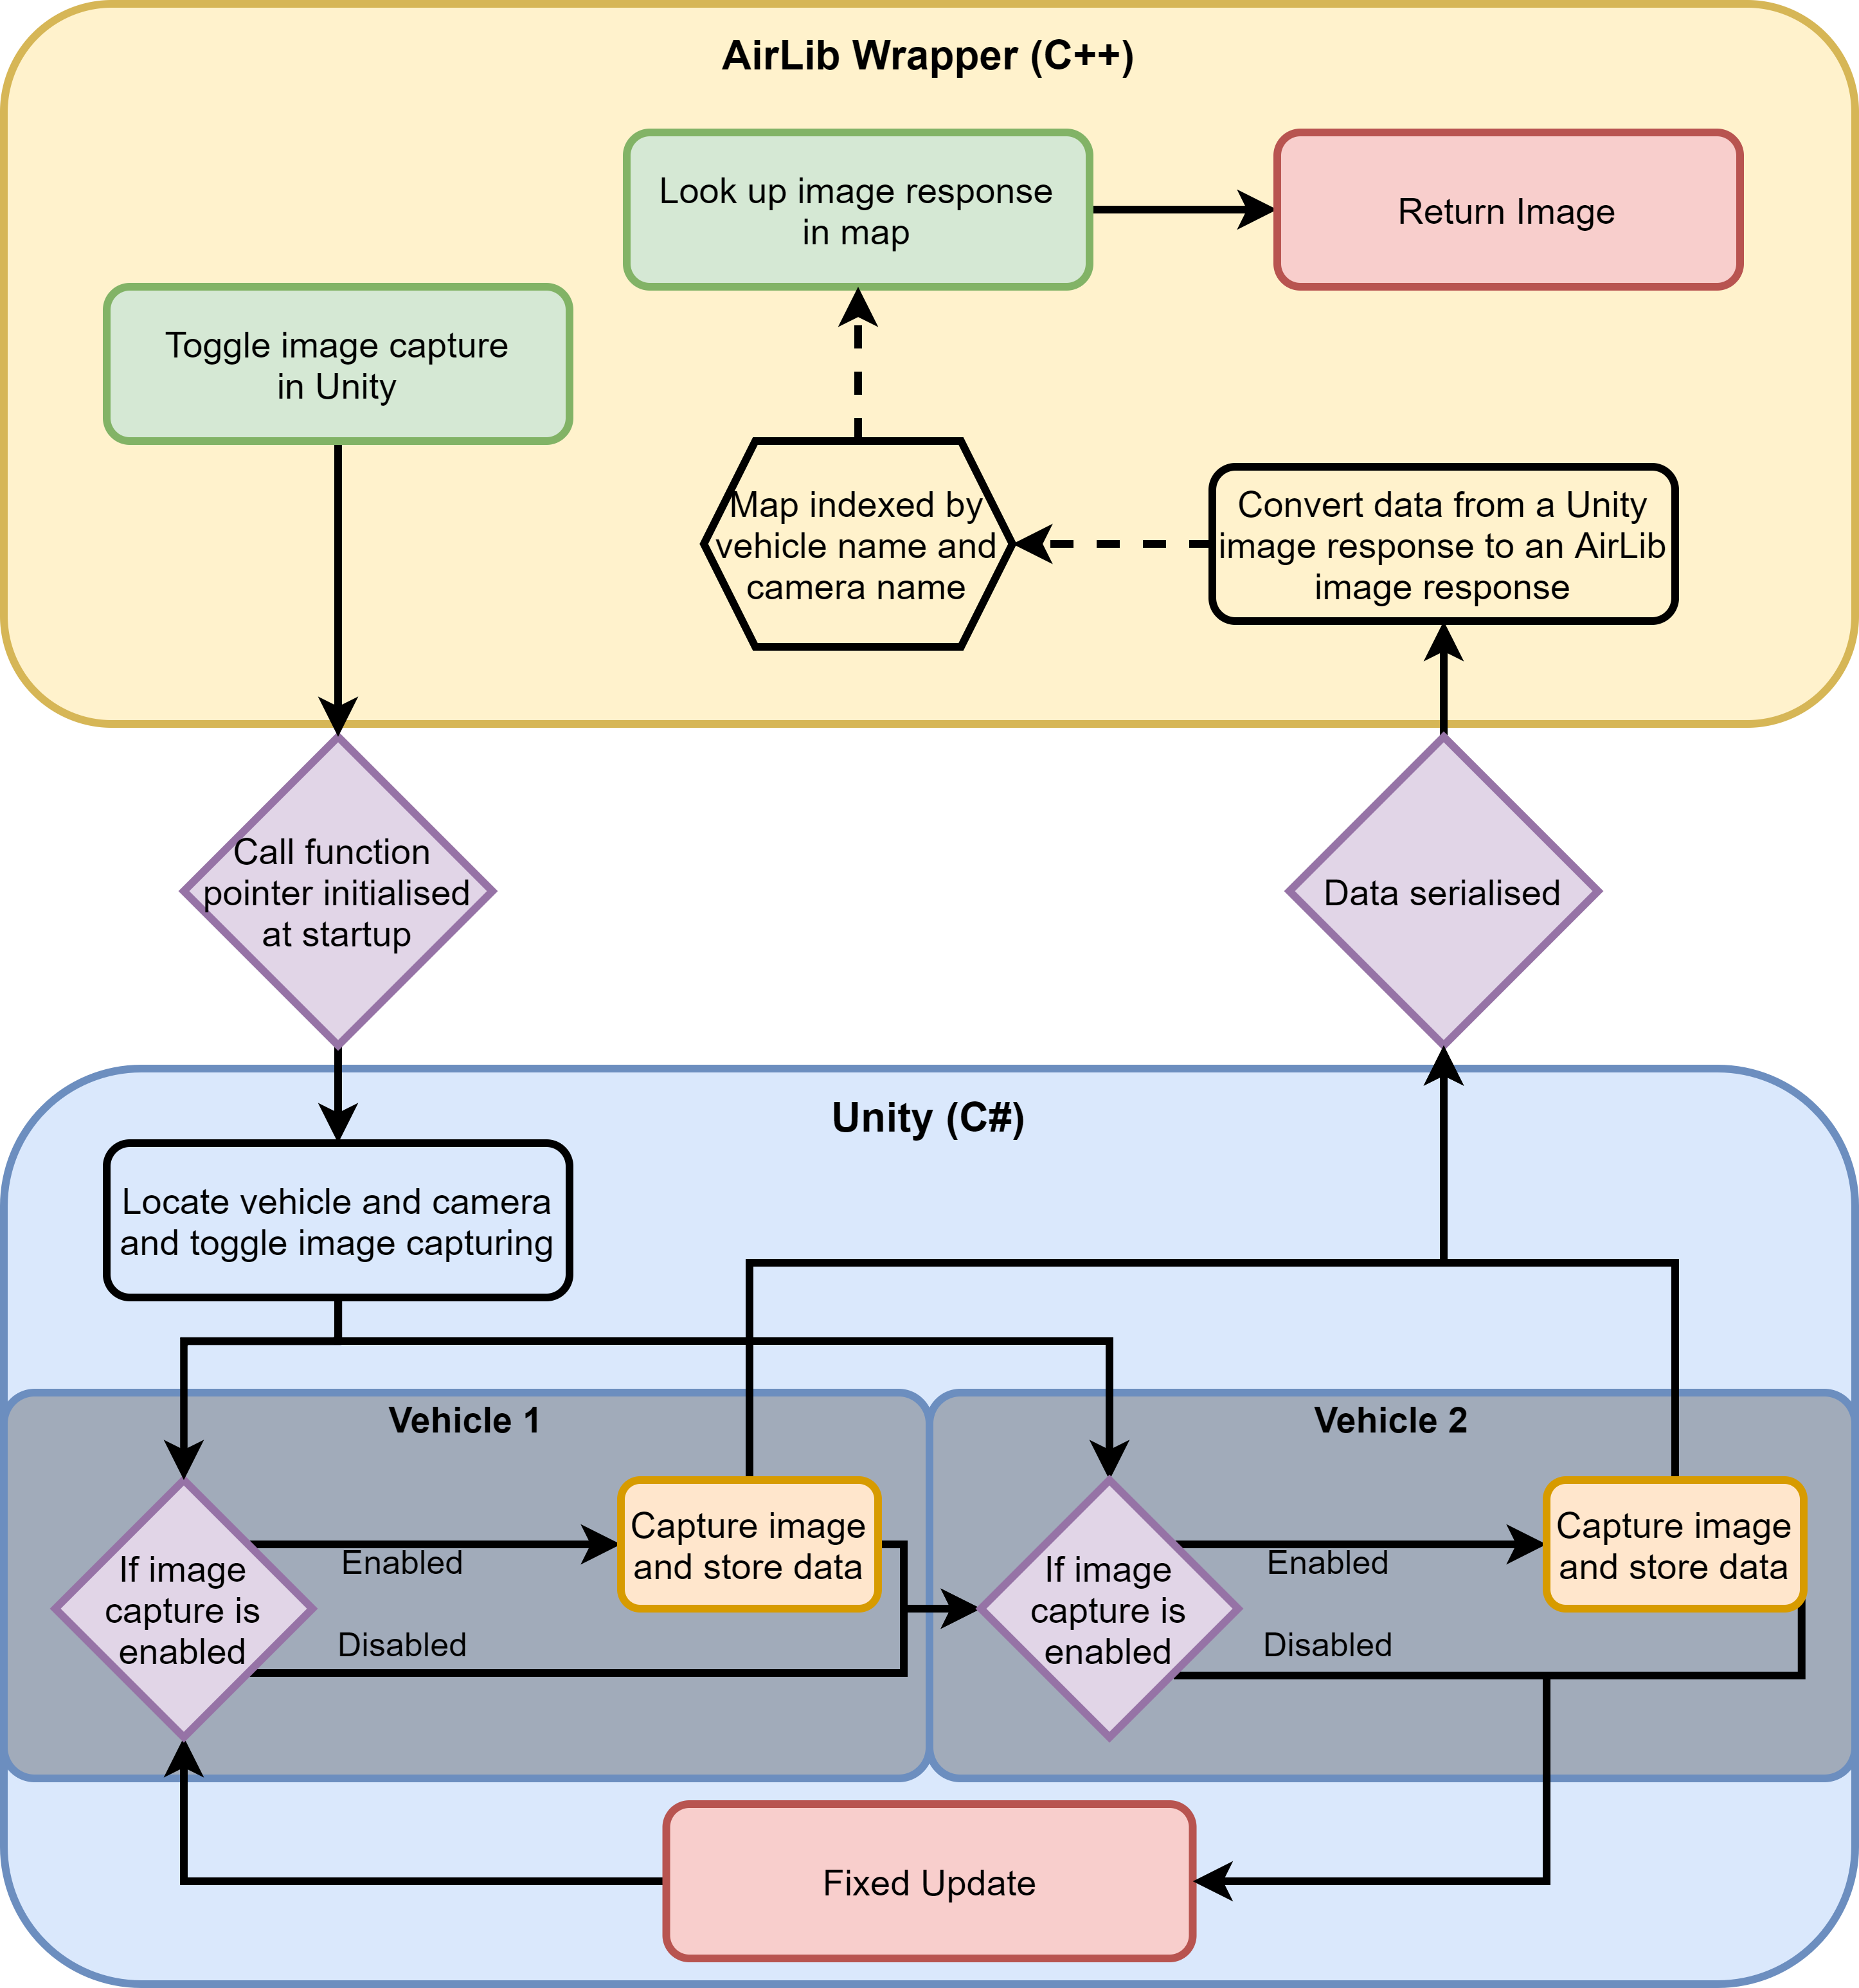
\includegraphics[width=1.0\textwidth]{06_Implementation/00_AirSim/Diagrams/imagecaptureUpdated.png}
    \caption{} \label{06:imageCaptureUpdated}
\end{figure}

\subsection{Adding Pedestrians}
This section will cover how pedestrians were added to the simulator. Pedestrians are one of the main forms of traffic wanted in this simulator. The pedestrians would be controllable through APIs in the same way as vehicles. 

The first step was to figure out how to create the pedestrians. The first option would be to use the standard Unity objects to create a character. This would be a simple capsule with a face. This would have been a bit simple for this project and having something more human-looking would be preferable. Another alternative was to download characters from mixamo\footnote{\url{ https://www.mixamo.com/}}. Mixamo is a technology company owned by Adobe which designs 3D characters and animation. The advantage of using Mixamo is that the characters come with a large range of animations as well as looking like humans. The disadvantage was having to download a large number of assets. Another way of creating character would be with the Unity character generation tool known as UMA2 (Unity Multipurpose Avatar). This allows for the character to have a variety of different shapes and attires. UMA can generate random models or they can be generated manually. Figure~\ref{} in the appendix shows some of the settings available. UMA  Figure~\ref{06:umaCharacters} shows some randomly generated characters inside Unity. These models will be used as the pedestrians. 

The next problem that had to be resolved was how to control the pedestrians. This was surprisingly simple. A character control script was already downloaded from the asset store when trying to use the Mixamo characters. Simply attaching this control script as well as the animation controller from the same asset made the characters run around. To make them walk, slowing down the direction speed worked. Another designed choice was made to have the controls for the pedestrians work similarly to the vehicles, i.e. pressing left and right would rotate the pedestrian rather than have it walk sideways on a grid. 

To make the pedestrians separated from the vehicles the server was divided into three components, the game server, pedestrian server and vehicle server. This was explained in the design chapter (Subsection~\ref{05:dividingServer}). Most of the basic APIs such as fetching available pedestrians, controlling the pedestrians and image capturing had to be reimplemented. These features were done similarly to how they work for the vehicles. The main difference being the struct with control commands being different. 

The next issue to be resolved was how to efficiently have UMA as a part of the project. UMA2 is over 500 MB and it would be unnecessary to have all of this pushed to GitHub. The solution was instead to have UMA as a requirement from the asset store. Prefabs were then created which would interact with the downloaded code. Script relating to AirSim would then be attached to these objects. 

Another small design decision that was made was how the cameras should behave. The animations make the pedestrians casually look around when standing still. To avoid this being an issue, the cameras are fixed facing forward from each eye. This means that the cameras are completely still when the pedestrians are walking. 

Overall the pedestrians took the most time to add to this project. Including dividing the server there was a lot of code that had to be changed throughout AirSim. One of the main challenges was that Unity does not display the error if there was an error caused by the AirLib DLL file. This made debugging the servers very difficult. Another issue that had to be resolved was that the original Unity version was too old to use all the UMA features. Updating Unity to a new version meant resolving other issues in AirSim and downloading outdated extensions. 
\begin{figure}[H]
    \centering
    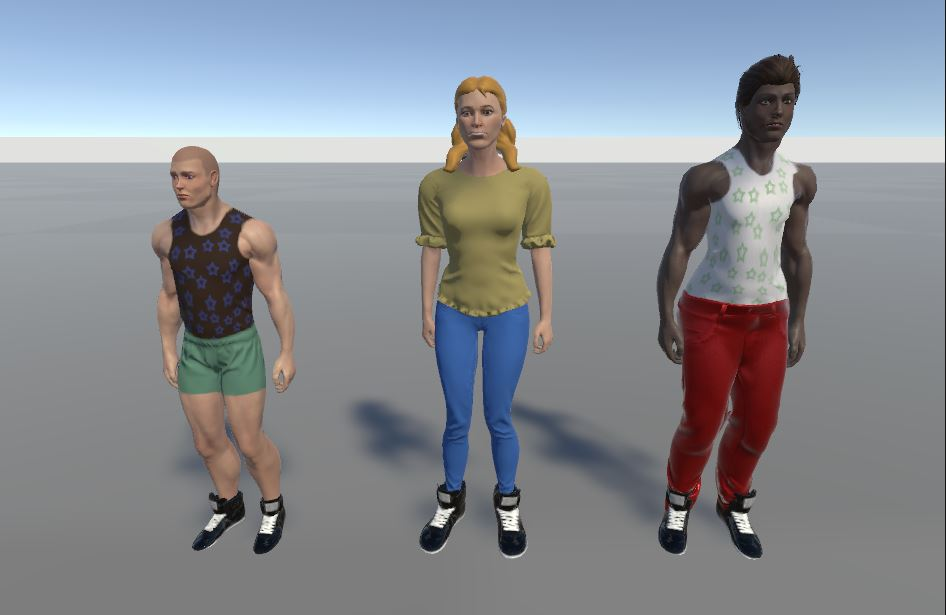
\includegraphics[width=0.6\textwidth]{06_Implementation/00_AirSim/Diagrams/RandomPedestrians.JPG}
    \caption{Randomly generated pedestrians using UMA2. UMA can be extended further by downloading additional assets which will add additional clothes, hair styles and more. UMA also allows for custom looking characters.} \label{06:umaCharacters}
\end{figure}

\subsection{Additional APIs}
This section will look at what additional APIs were added or modified.  It is worth noting that some of these features took a long time to add as they had to be done completely from scratch, whilst others could be done in less than an hour.

\subsubsection{Vehicle APIs}
\begin{enumerate}
    \item Updated \emph{enableAPIControls} - This is used to toggle the driving mode from through the API or manual inside the simulator.
    \item Updated \emph{simPrint} - Prints a debug statement from the vehicle.
    \item Added \emph{getVehicleTypes} - This returns a list of strings of the available vehicle types. This required significant changes to the simulator with roughly 15 files changed and 150 lines of code. The list of strings get converted into a char arrays with null terminated strings in C\# and then converted back into C++ strings in AirLib. Characters in C# are 16 bits, so every other character is skipped when reading the char array in C++.  This whole process was illustrated in Figure~\ref{05:stringList}. The commit with this can be found here\footnote{\url{https://github.com/tobhil98/MastersProject-AirSim/commit/22ab7c}}. A lot of time was spent trying to pass the arrays of strings from Unity to AirLib and then AirLib to Python.It is also worth nothing that this list could be extended with autonomous wheel chairs and other entities that would need the same controls and sensing abilities as a car. 
    \item Added \emph{simGetAllVehicles} - Returns a list of all vehicles in the scene. This is based off the getVehicleTypes API. 
    \item Updated \emph{setCarControls} - Updated how this was handled in Unity with several vehicles. Struct of car controls is passed from Python to Unity. 
    \item Updated \emph{getCarState} - Updated to handle several vehicles. Returns information about the car state such as speed, direction and location. 
    \item Added \emph{simGetLidar} - Added an API to fetch values form a Lidar beam. This is implemented in Unity using a ray cast to measure the distance to another object. Ideally this would be configurable in the request, but currently the beam is always from fixed points. 
    \item Updated \emph{simGetImages} - Fetches images using coroutines in Python. Decodes them and stores images in a dictionary indexed by the vehicle and camera name.
    \item Added \emph{simGetCameras} - Gets the names of the available cameras attached to the vehicle. 
\end{enumerate}

\subsubsection{Pedestrian APIs}
\begin{enumerate}
    \item Added \emph{ping} - Shows there is a connection with the pedestrian.
    \item Added \emph{reset} - Reset the pedestrian back to its original starting state.
    \item Added \emph{setPedestrianPose} - Sets the pedestrian position and rotation.
    \item Added \emph{getPedestrianPose} - Gets the pedestrian position and rotation.
    \item Added \emph{enableAPIControls} - This is based off the vehicles API. 
    \item Added \emph{simPrint} - Prints a debug statement from the pedestrian9.
    \item Added \emph{simGetAllPedestrians} - Returns a list of all pedestrians in the scene. This is based off the getVehicleTypes API. 
    \item Updated \emph{simGetImages} - Fetches images using coroutines in Python. Decodes them and stores images in a dictionary indexed by the vehicle and camera name.
    \item Added \emph{simGetCameras} - Gets the names of the available cameras attached to the pedestrian. 
\end{enumerate}


\subsubsection{Server APIs}
\begin{enumerate}
    \item Added \emph{ping} - Shows there is a connection with the server.
    \item Added \emph{getTickRate} - Fetches the current simulator tick rate in frames per second.
    \item Added \emph{simAddVehicle} - Explained in detail above how it is implemented. Spawns in a vehicle at a rotation at a specific location
    \item Added \emph{simAddPedestrian} - Spawns in a random pedestrian.
    \item Added \emph{simRemoveVehicle} - Removes the vehicle.    
    \item Added \emph{simRemovePedetrian} - Removes the pedestrian.
    \item Moved \emph{simPause} - APIs used to control the simulation speed. Moved from the old vehicle server.
    \item Moved \emph{simLogPrint} - Sends a debug print statement to Unity. 
\end{enumerate}


\subsection{Minor Features Added}
This section will briefly list other features added to the simulator. 
\begin{enumerate}
 \item \emph{Camera movement} - To be able to look around the simulator several different camera configurations have been implemented. These are to use in the simulator and cannot be controlled through APIs. One option is a free camera which allows the user to fly around the environment. The second option is to follow a specific entity. These options have been mapped to three number keys, key 1 for free movement, key 2 to follow vehicles and key 3 to follow pedestrians. When following vehicles or pedestrians the user can cycle through them by pressing tab (or shift+tab to cycle the other direction). The user can also easily move from following an entity to free camera movement by pressing the left shift key. 
 \item \emph{Rebuild script} - This is a simple update to the build script that compiles the AirLib dll. This change allows for faster compile time. This is very beneficial as it reduces the time to compile from over 10 minutes to just over 1 depending on the change made to the code. This change was a very small change to the build script which meant only files that had to be recompiled were recompiled, instead of rebuilding the whole project. 
 \item \emph{Upgraded Unity version} - The version Unity version used by AirSim by default is 2019.3.12, however there is a bug in this version which means internal projects cannot communicate with each other. The main issue here was that there was no way of communicating with the UMA code from the AirSim code. This was resolved by upgrading the version to 2019.3.13. This introduced a bunch of dependency issues as well as a couple of code issues that had to be fixed. This change should not impact future pull requests from the master repository as most features that are commonly used were backwards compatible. 
\end{enumerate}
%freecam and change between vehicles and entities
%Added global print from server - First thing to be added to get used to the codebase. 
%Rebuild script?
\subsection{Other Features Considered}
This section will briefly mention other features considered when adding features to Unity. The main reason for not adding these was in the interest of time.
\begin{enumerate}
\item \emph{Unity Navmesh}\footnote{\url{https://docs.unity3d.com/Manual/nav-CreateNavMeshAgent.html}} - This would allow pedestrians and vehicles to navigate around autonomously without needing to train a network. The navigation mesh can be laid on any surface to indicate where entities can go.
\item \emph{Unity Cloud Build}\footnote{\url{https://unity3d.com/unity/features/cloud-build}} - This is a framework that would allow testing the system online. However, this requires an advanced Unity license, so was not feasible for this project.
\end{enumerate}


\subsection{Extensibility}
The advantage of using AirSim and Unity is that the whole system is very flexible. As mention in the design chapter (Chapter~\ref{design}), AirSim allows for a variety of different languages to interact with the APIs. The whole project has made sure that future extensions should be simple to add if needed. This section will briefly look at how the existing features can help extend a future design.

\begin{enumerate}
\item \emph{Additional APIs} - This can be slightly complicated depending on the API. The API to base the new API off should be simGetImages. This is because it passes a struct of arguments to Unity, does some complex processing and passes a struct back. The struct has to be converted to different formats as it goes through AirSim as was shown in Figure~\ref{05:stringList}.
\item \emph{Additional Vehicle types} - This is done by adding the control script to the vehicle and then adding the prefab to the asset manager in the scene. To get all available vehicles for example the user could use the getVehicleTypes API which returns the names of the different types.  
\item \emph{Competly new type like wheelchairs} - This can either be added like an additional vehicle type with different physical properties. This would then have to use the same vehicle controls. It is also easy to look at how the pedestrian server works. Now the servers have been divided, creating more similar servers to how pedestrians were created is simple.  
\item \emph{Customise cameras} - Adding additional cameras to an object is done by creating a camera object onto the model and renaming the camera. The vehicle controller will find the object called Capture Cameras and iterate over the object to find all the cameras. The fetch available camera API listed above fetches all cameras attached to a specific object, so different vehicles can have a different number of cameras. 
\end{enumerate}

As AirLib works as a plugin to Unity, all Unity features are still available to use. This means adding something like VR or AR to the simulator should not be difficult if required.  

% Different vehicle designes by simply attaching the scritps
% Number of cameras
% Creating new types, for example autonomous chairs is simple by 




% Why did this not already exist
% •	Used to use config file. Not needed before.
% What changes had to be made
% •	Adding a new API to spawn vehicles, with position, rotation and name as arguments. 
% •	Server is connected to vehicle. Start server without vehicle
% How was the change made.
% •	Add APIs like diagram to spawn vehicles. 
% Challenges faced.
% •	Function pointers not bound by that point in time. Move vehicle spawning. 
% •	Issues with the threading

% Any limitations or known issues?



\section{ML-Agents}
\subsection{Reinforcement Learning}

\subsection{Learning by Demonstration}

\subsection{Collaboration Learning}

\section{Maps and environments}
This section will look at different ways of importing or creating city maps in Unity. The purpose of this is to give the agents an environment that more accurately replicates the real world. There are two main ways of doing this. The first option is loading the maps in at runtime. This option would give the agent an unbounded area to navigate around. The second option is to create a Unity asset. This option allows the user to create a 3D model of the environment and load the object into the scene at compile time.  
\subsection{Unity Map SDKs}
There are several different Map SDKs available for Unity. The advantage of using an SDK over an asset is that it allows the user to navigate any place. As the agent navigates around, new areas of the map will be loaded. Another advantage is that the maps are updated and can provide real information such as traffic congestion. A disadvantage is that these maps need to be download at runtime. This requires access to the internet and can be slow to load. Another disadvantage is that these services are subscription-based. This means that there is a limit to the number of requests that can be made \footnote{\url{https://www.mapbox.com/pricing/}}.

\subsubsection{Google Maps Unity SDK}

Google Maps Unity SDK contains several developer tools which allow the user to create mobile games with real-world locations\cite{google_maps_sdk_platform}. The advantage of using this SDK is that it provides additional tools such as the ability to extract place IDs as well as the name of geographic features. The SDK also includes real-world features from particular locations. The disadvantage with the Google Maps SDK is that it currently only supports mobile applications. The simulator is primarily designed to run on a computer so this SKD would therefore not work for this project. 

\subsubsection{MapBox Unity SDK} 
The MapBox Unity SDK is a toolbox that can be used to create worlds with continuous road networks, points of interests and street labels. It also can use satellite images to create realistic terrain. The advantage of the MapBox SDK is that it is free and easy to set up. The disadvantage is that the generated textures do not look as good as other map options. There are also some missing buildings as can be seen from Figure~\ref{maps:figure:MapBox}. MapBox does allow the users to modify the maps online, but this has to be approved before the maps are updated.  

\subsubsection{Wrld3D Unity SDK} 
Wrld3D Unity SDK is a dynamic 3D mapping platform that can replicate indoor and outdoor environments. Similar to the SDK created by Google, famous landmarks and features are recreated. The SDK comes with a variety of different APIs. These include,  for example, select and highlight buildings, enter and exit indoor maps and visualise the transport network. As can be seen from Figure~\ref{maps:figure:Wrld3D}, the applied textures look better than the textures provided from the MapBox SDK (Figure~\ref{maps:figure:MapBox}). Wrld3D costs 20 USD per months making it one of the more expensive options. The maps are however more visually appealing than the other options. In addition, the maps have smoother and more accurate surfaces making it easier for the simulation, compared to for example the Google 3D maps loaded into Blender (Figure~\ref{maps:figure:GoogleMaps}).

\begin{figure}[!htbp] 
\centering
\begin{minipage}[t]{.45\textwidth}
\centering
\begin{subfigure}{\textwidth}
        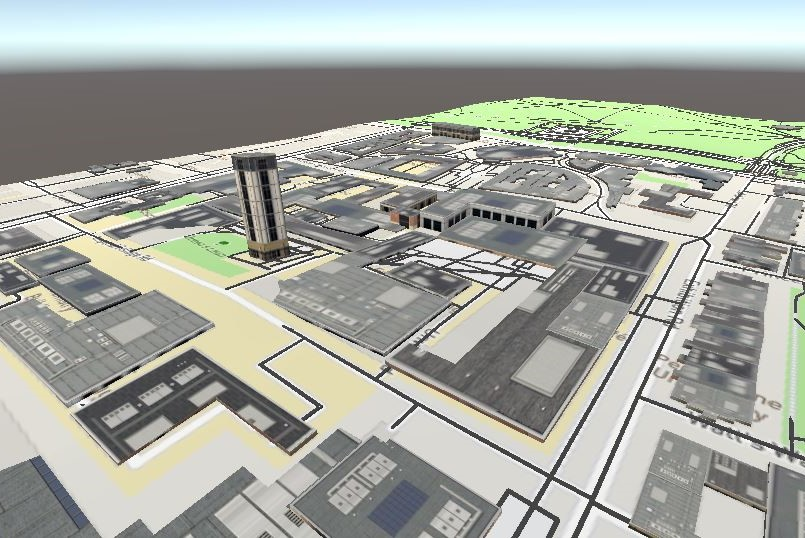
\includegraphics[width=\linewidth, left]{06_Implementation/00_Maps/Images/MapBox1Cropped.JPG}
        \caption[Map created using MapBox]{Imperial Campus loaded into Unity using the MapBox SDK. All objects have been given an arbitrarily texture. Also, the building scale is off.}
        \label{maps:figure:MapBox}
    \end{subfigure}
\end{minipage}
\qquad
\begin{minipage}[t]{.45\textwidth}
    \centering
    \begin{subfigure}{\textwidth}
        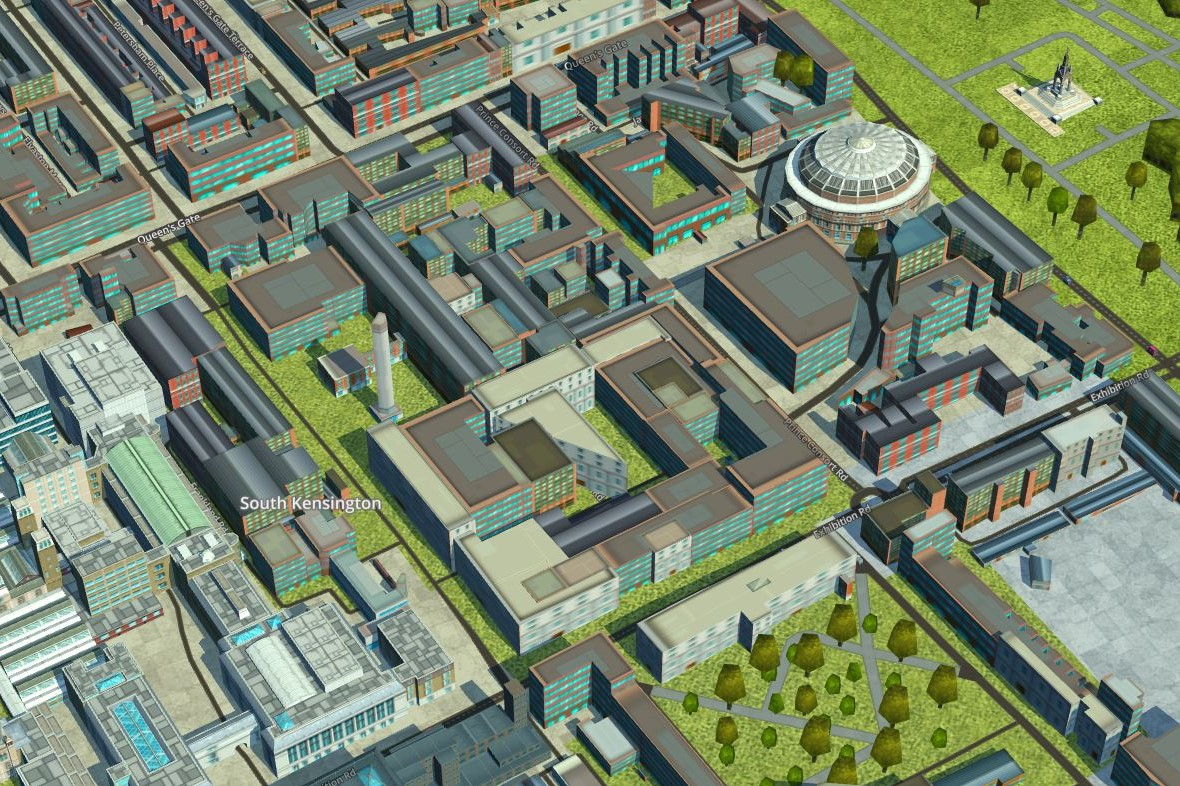
\includegraphics[width=\linewidth, right]{06_Implementation/00_Maps/Images/Wrld3D1Cropped.JPG}
        \caption[Map created using Wrld3D]{Wrld3D has a tool online where you can look at the map before purchasing the SDK subscription. The image is a screenshot from this tool\footnote{\url{https://maps.wrld3d.com/?mapscene=632ba4b}}.}
        \label{maps:figure:Wrld3D}
    \end{subfigure}
\end{minipage}
\end{figure}

\FloatBarrier
\subsection{Unity Map Assets}
Loading map assets into Unity requires more initial work as they require 3rd party tools. An advantage of creating assets is that it gives the user the freedom to modify the maps before importing them into the simulator. Blender is commonly used as a free program for creating and modifying 3D models\cite{MendozaGuevarraEzraThess2020CGEi}(Section~\ref{blender}). Another advantage is that the maps are loaded at compile-time. This means that the model loads quickly and the simulator does not require access to the internet. The disadvantage is that the agents will be limited to only that environment. Large maps can be computationally hard to render and cause the simulator to lose performance. This is due to the large polygon count which requires more memory and CPU usage. (More information in the User Guide Section~\ref{UserGuide}). Depending on the method used to create the models, creating better-looking options using Blender can be very time-consuming and requires additional skills to use the tool. 


\subsubsection{OpenStreetMap2World}
OSM2World is an open-source program that takes maps generated by Open Street Map\footnote{\url{https://www.openstreetmap.org/\#map=16/51.4976/-0.1715}} and them into object files which can be loaded into Unity. There are several advantages of using OSM2World to create assets. Firstly, this program is easy to set up and generate object files. The user can either use the GUI or use the CLI. Another advantage is OSM2World creates objects which consist of several layers. These layers are different features the world consists of, for example, roads, junctions, footpaths and buildings. Having these layers allows the user to interact with each of them separately. Users can manually modify these layers on the OpenStreetMap website\footnote{\url{https://www.openstreetmap.org/}}.

The disadvantage of using OSM2World is that it does not allows to render the objects with texture in Unity. It is also difficult to make adjustments to the environment without using another tool like Blender. These adjustments could be updates that the user would like to have for their environment, but are not changes that should be uploaded to the map itself, like adding additional walls to close the area.

\begin{figure}[H]
    \centering
    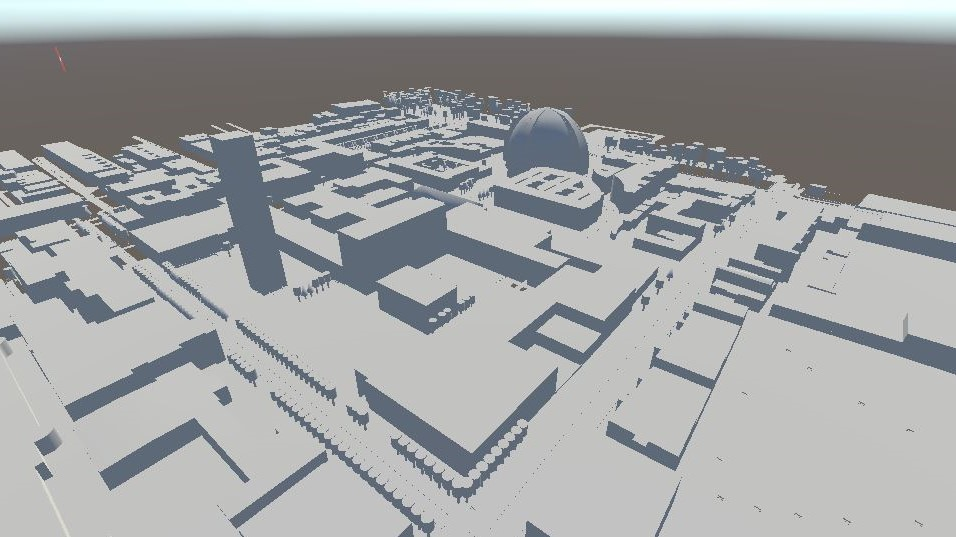
\includegraphics[width=0.65\textwidth]{06_Implementation/00_Maps/Images/OSM1Cropped.JPG}
    \caption[Map created using OpenStreetMap2World]{South Kensington Campus created using OpenStreetMap2World loaded into Unity}
\end{figure}

More information on how to create an object file from OpenStreetMap can be found in the user guide (Chapter~\ref{UserGuide} in the appendix).
\subsubsection{BlenderGis}
BlenderGis is an open-source Blender addon that allows users to import GIS (geographic information system) files. The addon includes the option to download a map area from either Google or OpenStreetMaps directly into Blender without having to download the GIS files externally. One advantage of using BlenderGis over OSM2World is that GIS files include the world heightmap. This means that this method can more accurately map the terrain. 

BlenderGIS can also be used to import structures and buildings like OSM2World, and the quality is somewhat similar. This Blender addon also includes the different map layers like OSM2World, but there are not as many options. Different kinds of roads, junctions and so on are all just marked as highway. 

The main advantage of using BlenderGIS over OSM2World is that BlenderGIS allows adding texture to the map. The satellite image is projected onto the map ground, making the scene much more recognisable. There is also a way of projecting the textures onto the buildings. As the satellite images are only taken from above, there is no way to add texture to the sides of the buildings without using a generic front. 

\begin{figure}[H]
    \centering
    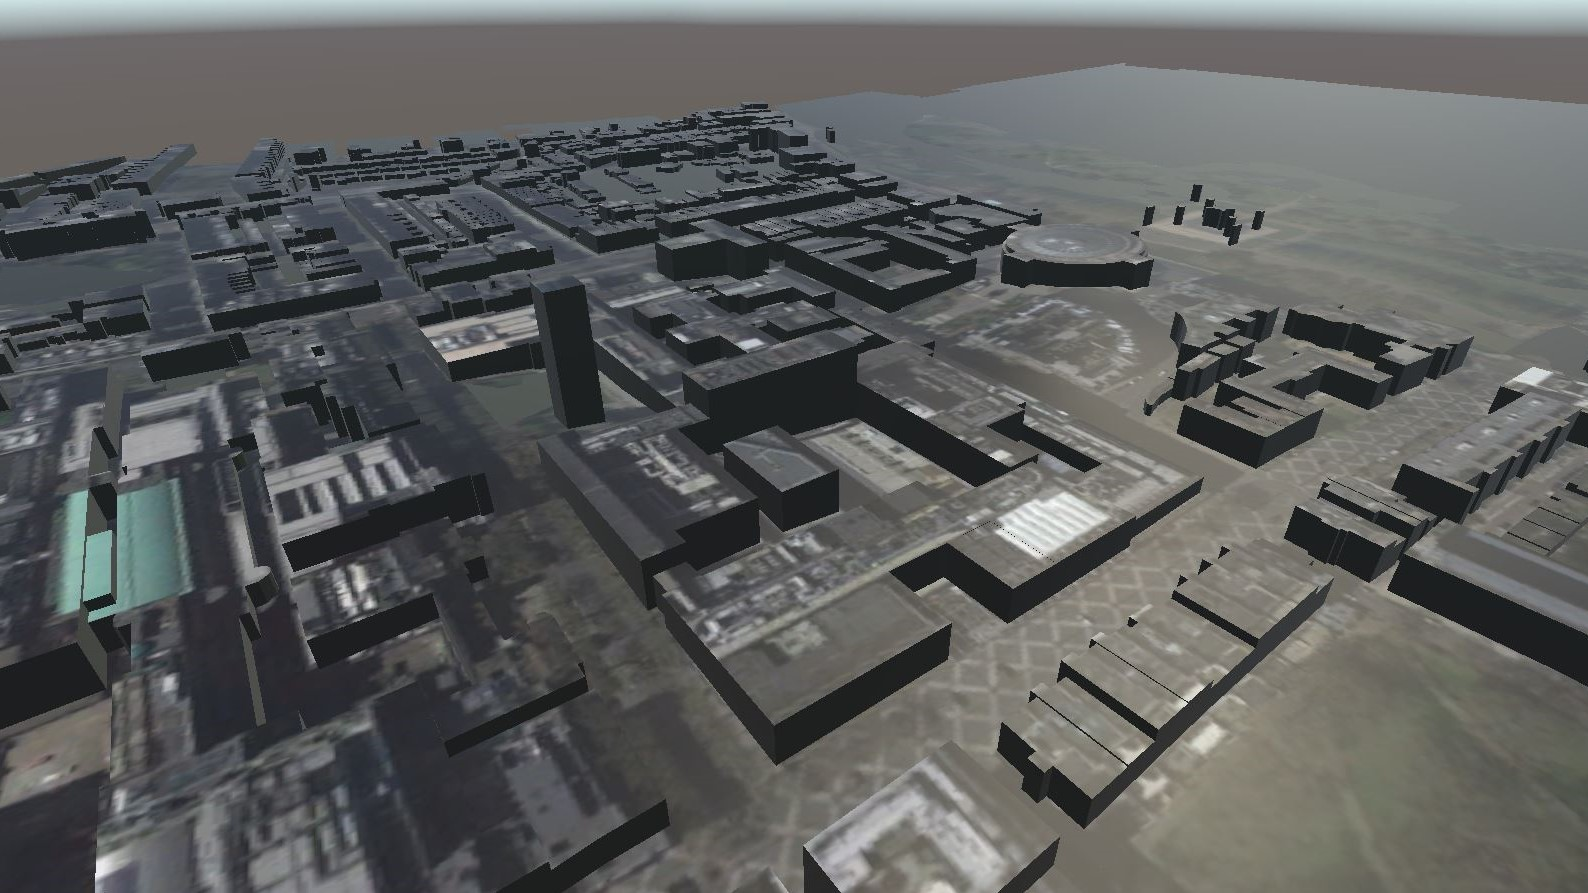
\includegraphics[width=0.65\textwidth]{06_Implementation/00_Maps/Images/BlenderGis1Cropped.JPG}
    \caption[Map created using BlenderGis]{South Kensington Campus created using BlenderGis, then load into Unity. Some buildings are missing and the texture looks quite flat.}
\end{figure}

\subsubsection{Google Maps GPU Intercept}
For personal projects, Google Maps' 3D view can be imported into Blender. These steps are quite convoluted, but the user guide (Chapter~\ref{UserGuide} in the appendix) explains how to do this in more detail. In essence, renderDoc can be used to intercept the data going from Google Chrome to the GPU. This data can then be loaded into Blender by using MapsModelImporter\footnote{\url{https://github.com/eliemichel/MapsModelsImporter}}. This step can take a long time as many polygons have to be loaded. Once the map has been imported into Blender, the user can freely update the model. One update that should be made is to reduce the polygon count. Blender has a tool for this. This is needed as there are several thousand polygons, and this process can remove almost half without a noteworthy difference (Figure~\ref{maps:figure:GoogleMaps}). Finally, the model along with the textures can be exported to Unity. 

The advantage of using this method is that it looks a lot better than the other options. There is also a lot more detail which makes the environment more realistic. This can be useful when training machine learning models as the trained model would not overfit to a perfect environment. 

However, there are several disadvantages to using this method. Firstly, creating maps using this method is a lot more time-consuming. Importing the map into Blender, then exporting it to Unity can take several hours due to a large number of polygons. This method is also a lot more computationally expensive when running in Unity, as each polygon has to be rendered. Secondly, the roads are not even and flat, as cars on the roads are incorporated into the model. This can be smoothed using tools in Blender, but this is once again time-consuming. The last disadvantage is that the model does not include map layers which the other method do. This means there is no way of distinguishing different objects, like buildings, trees and parked cars, apart. 

\begin{figure}[H]
    \centering
    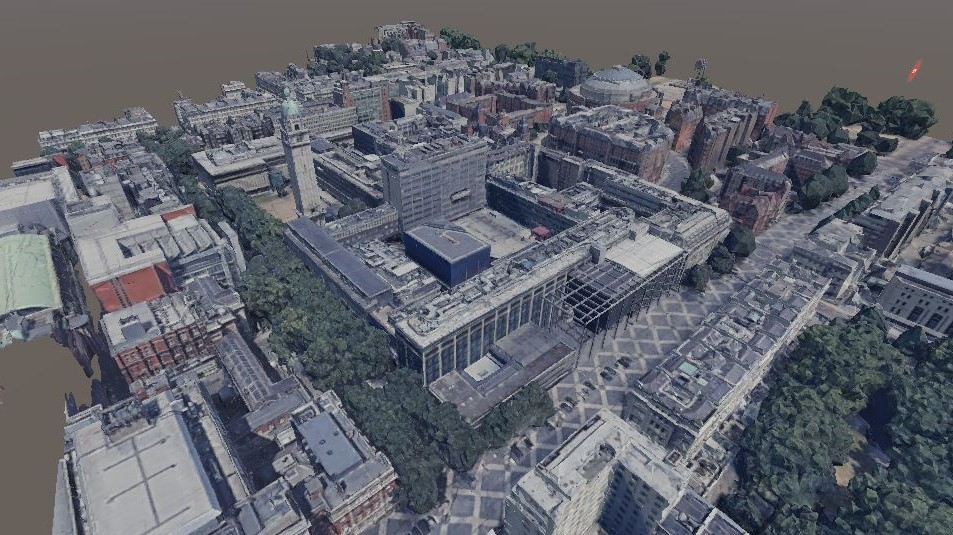
\includegraphics[width=0.7\textwidth]{06_Implementation/00_Maps/Images/Google5Cropped.JPG}
    \caption[Map created using Google Maps]{South Kensington Campus loaded from Google Maps into Blender, then exported to Unity. Number of polygons reduced by 60\%}
    \label{maps:figure:GoogleMaps}
\end{figure}

\subsection{3D World Scanners}
Another way to create an environment is to use a mobile application to scan the surrounding area. This will generate a 3D model which can be imported into Blender. Similar to the GPU intercept method, the created environments contain a very high polygon count and can have some rough edges.

There are several apps which does this, but most are not free. Display.land was widely used until it was taken down a few months ago. According to their website\footnote{\url{https://get.display.land/}}, the company has plans to release a new version soon. The best application found for Android turned out to be Scann3D\footnote{\url{https://play.google.com/store/apps/details?id=com.smartmobilevision.scann3d}}. It can produce simple models of objects, but struggles with larger areas. The quality of the output is not very good. According to different sources online, trnio\footnote{\url{https://www.trnio.com/}} works well for iOS, but this has not been tested. 


\subsection{Conclusion}
For this project using map assets rather than an SDK would be better. As the simulation is about the interaction between different kind of agents, an infinite map is not required. Using an SDK is a good alternative if the specification for the project changed and training agents at several different random locations became more important. The benefit of the faster loading time and not having to rely on an external API at runtime makes loading the environment as a Unity asset the best option. 

In regards to which of the asset methods to go for really depends on the task. For a visual demonstration, the optimal choice would be to overlay the data from Google Maps on top of the height map generated by BlenderGis. This can be seen in Figure~\ref{maps:figure:combined}. This approach would then allow for smooth roads whilst keeping the detail on the buildings and other structures. 

If the visual is not important, using something like BlenderGis would work well. This allows for a layered map as well as providing the terrain height. It is also easy to set up and use. 

\begin{figure}[H]
    \centering
    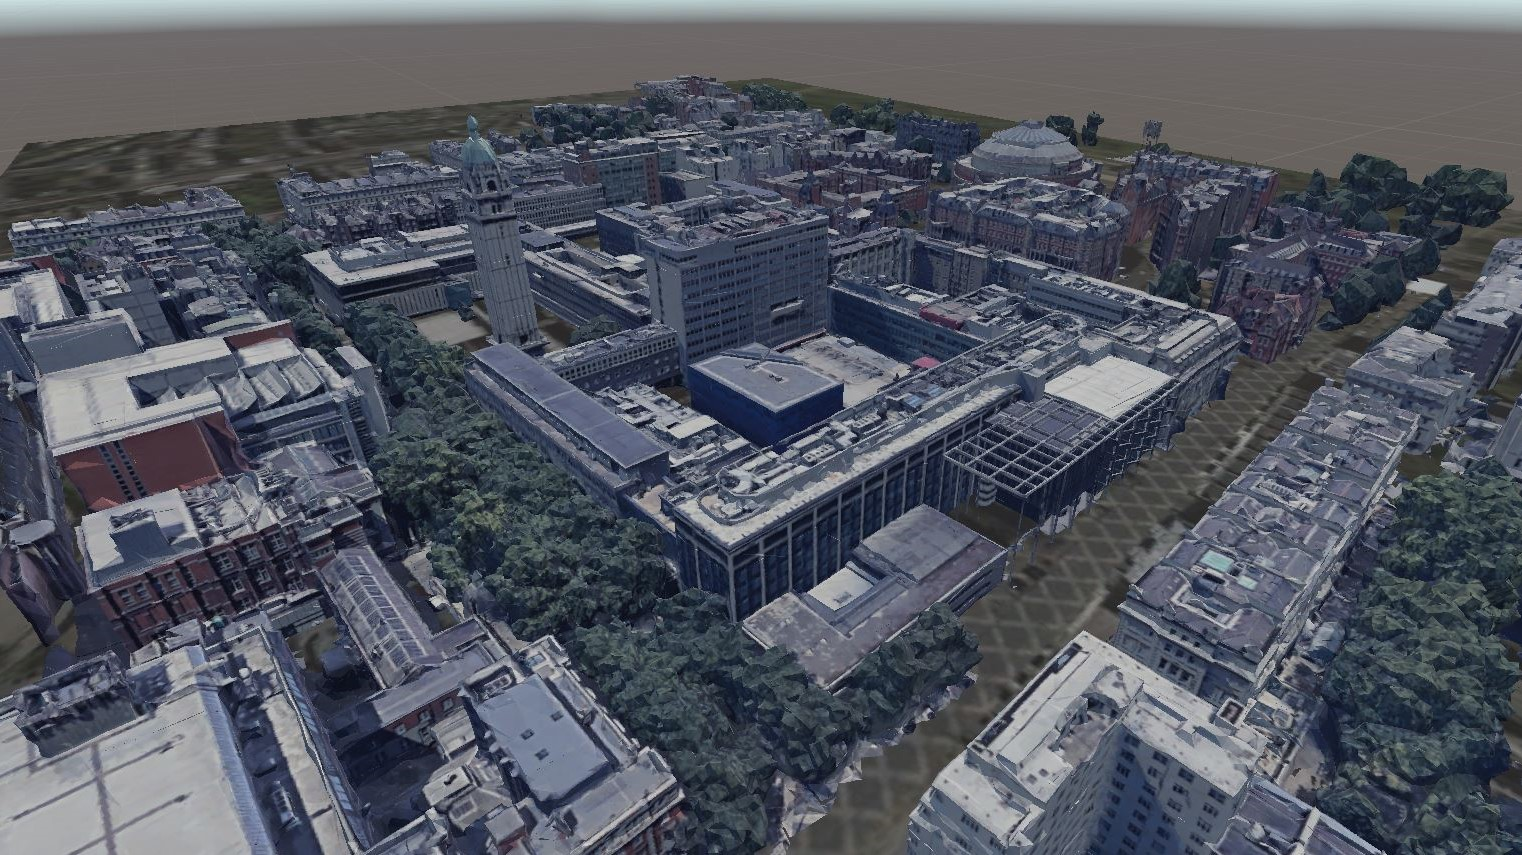
\includegraphics[width=0.7\textwidth]{06_Implementation/00_Maps/Images/CombinedCropped.JPG}
    \caption[Combined BlenderGis and Google Maps]{BlenderGis and Google maps combined. Allows for smooth roads whilst keeping the aesthetics of the buildings. Downside is that its computationally intensive to run and file size over 100MB.}
    \label{maps:figure:combined}
\end{figure}



% \subsection{AirSim}
% AirSim is missing pedestrians, and this has been the first and main priority for the time being. The plan is to add pedestrians in such a way that it will be easy to add cyclists and other mobile robots soon after that. As can be seen in the timeline (Section~\ref{timeline}) this is expected to take roughly 3 weeks. This is also due to the fact that other commitments have been pushed back slightly due to this Interim Report. In AirSim currently we have got a character added, but the character does not yet have any ability to be spawned in or controlled.
% \\~\\
% AirSim has a lot of available APIs, and the hope is to either incorporate them, or follow their specification when implementing our own. AirSim has a lot of documentation to help with this. There is also an active community where developers can go and ask questions. 
% \\~\\
% AirSim is built using both Unreal Engine and also Unity. For the time being the plan is to only use Unreal Engine. This is to prioritise rapid development rather than cross game engine compatibility. 
% \\~\\
% An advantage of using AirSim is that it could later allow us to use drones in the simulation. This is however not something that will be looked at yet and the feature will be ignored for the time being. 


%%%%%%%%%%%%%%%%% Testing
\chapter{Testing and Results}\label{results}
This chapter will look at the performance of the Simulator as a whole as well as the performance of the ML-Agents. As this is only a prototype the performance is not the most important aspect. The chapter will also look at how the simulator was tested.

% As this is an implementation project, most of the testing was discussed in the Implemenation section.  
\section{Simulator Performance}

\section{ML-Agents Performance}


%%%%%%%%%%%%%%%%% Evaluation
\chapter{Evaluation}
% When evaluating the simulator there will be some key features to look at:
% \\~\\
% The main one will be \textbf{usability}. It is important that it is easy to use the simulator. When evaluating the usability we will look at:
% \begin{itemize}
%     \item How to set up the simulator.
%     \item How easy it is to import maps.
%     \item How to add agents into the simulation.
%     \item How to configure these agents.
%     \item How to control these agents.
%     \item Are the APIs easy to use?
% \end{itemize}
% Documentation should be written to make it clearer in regards to the elements listed above. It could also be useful to ask someone else to try using these features to evaluate if the documentation is clear and intuitive. 
% \\~\\
% The simulator could also be evaluated on \textbf{feature richness}:
% \begin{itemize}
%     \item How much of the objectives (Section~\ref{Objectives}) have been implemented.
%     \item Are there any other needed features that have not been implemented.
%     \item Is there a variety of available agents, such as pedestrians and autonomous robots?
% \end{itemize}

% %\\~\\
% Finally, it is also worth evaluating the \textbf{performance}:
% \begin{itemize}
%     \item Memory usage
%     \item Frame rate
%     \item Responsiveness
% \end{itemize}
% Some simulators had a clear impact on performance when several agents were spawned at once. It is important to make sure that the simulator is still usable for a small number of entities. 




%%%%%%%%%%%%%%%%% Evaluation
\chapter{Conclusions}
Overall this project successfully implemented a traffic simulator that could simulate mixed traffic as required. AirSim was selected as the simulator to extend over many others. Most of the missing features were then added to the simulator. AirSim had a big diverge from the original version when the server was divided into 3 parts. This was done to allow for future possibilities where each vehicle would have its server. This split also made it simple to add completely new types of vehicles with a different set of controls and APIs. 

The next big part of the project was to train the ML agents. The vehicles are far from perfect, but they have definitely learnt to follow limit contact with the wall and drive towards the target. 

For this project, most of the time was spent trying to get used to tools and programs. It took a long time at the starts to get an understanding of how the AirLib code works as there was no guide over the code architecture. Trying to understand the code base whilst having to do other unrelated work made it harder. Also, getting used to tools like Unity and Blender took time. Some time was used customising the environments in Blender to make them look better which could be used in a demonstration.

The biggest coding challenge was dividing the server. This meant that a lot of code had to be understood, moved or modified. This was important to get working as making the simulator more easily extendable was a key part. 

A lot of time was spent researching and understanding GAIL and collaboration learning for the ML-Agents part of the project. Most evening several models have been training on lab computers. Due to slow internet and not being able to go into uni, made it very difficult to fix bugs, as uploading the build took several hours, and the environment could not be trained on this computer. 

Overall this was an ambitious project that has tried a lot of different tools and features and combined them into one simulator. For a perfect system, more APIs could have been added to control the vehicles and the ML agents could have had better performance. However, this project was not looking for an optimal solution, but rather a prototype consisting of a large range of features. 

\chapter{Further Work}
This chapter consists of two sections. The first section will look at what needs to be done to the existing simulator to improve the quality. The second section will look at future use cases for the simulator.  

\section{Simulator extension}
The first thing would be to further improve the ML-Agent model. The existing model can drive around, but not in a reliable way. More training and further parameter tuning would be needed. Also, training the pedestrians so that the interaction between pedestrian and vehicles can be simulated. Currently, the interaction is only handled through the APIs.

The next step would be to add more controlling APIs to the simulator. Being able to give the pedestrians more relaxed information such as walk forward but pause if something is in front would be very beneficial. This would be the same for the vehicles. Currently, the simulator is only a platform where all of these things have to be manually controlled or controlled through external programs using the APIs.

Another big improvement would be to optimise the video stream even further. This could potentially be done by using UDP streaming. However, as the image capturing has to be done on the main thread, this could be an unsolvable problem until Unity upgrades its game engine. 

Lastly, there are a lot more features in AirLib which have not yet been added to AirSim. More advanced weather, additional sensors and several APIs that exist in Unreal Engine but not in Unity could be added. 


\section{Use cases}
One option would be to try to use the simulator alongside an external sensor, like a traffic camera, to create a digital twin of the real environment. There are several use cases for this. Firstly, it could detect dangerous driving and report it to the police. This could both make people drive more safely as they know they are being surveyed, as well as making it possible to stop dangerous driving early on. It could also be used to track dangerous traffic junctions to monitor and detect near-collisions. 
\\~\\
Another option could be to simulate an autonomous wheelchair that exists in the Imperial Robotics Lab. By modelling the wheelchair in AirSim we could try to create an autonomous system and then compare it to the behaviour in real life.
\\~\\
A third example could be to try to train a machine learning model for an autonomous robot so that it could navigate around crowded places with cars and pedestrians \cite{ChaoQianwen2015Vifm}. 
\\~\\


%%%%%%%%%%%%%%%%% User Guide


\newpage
\bibliographystyle{IEEEtran} %agsm
%\nocite{*}
\bibliography{
    references,
    06_Implementation/references
}

\begin{appendices}
\appendix
\chapter[Background Theory Diagrams]{Background Theory}
\begin{figure}[H] 
    \centering
    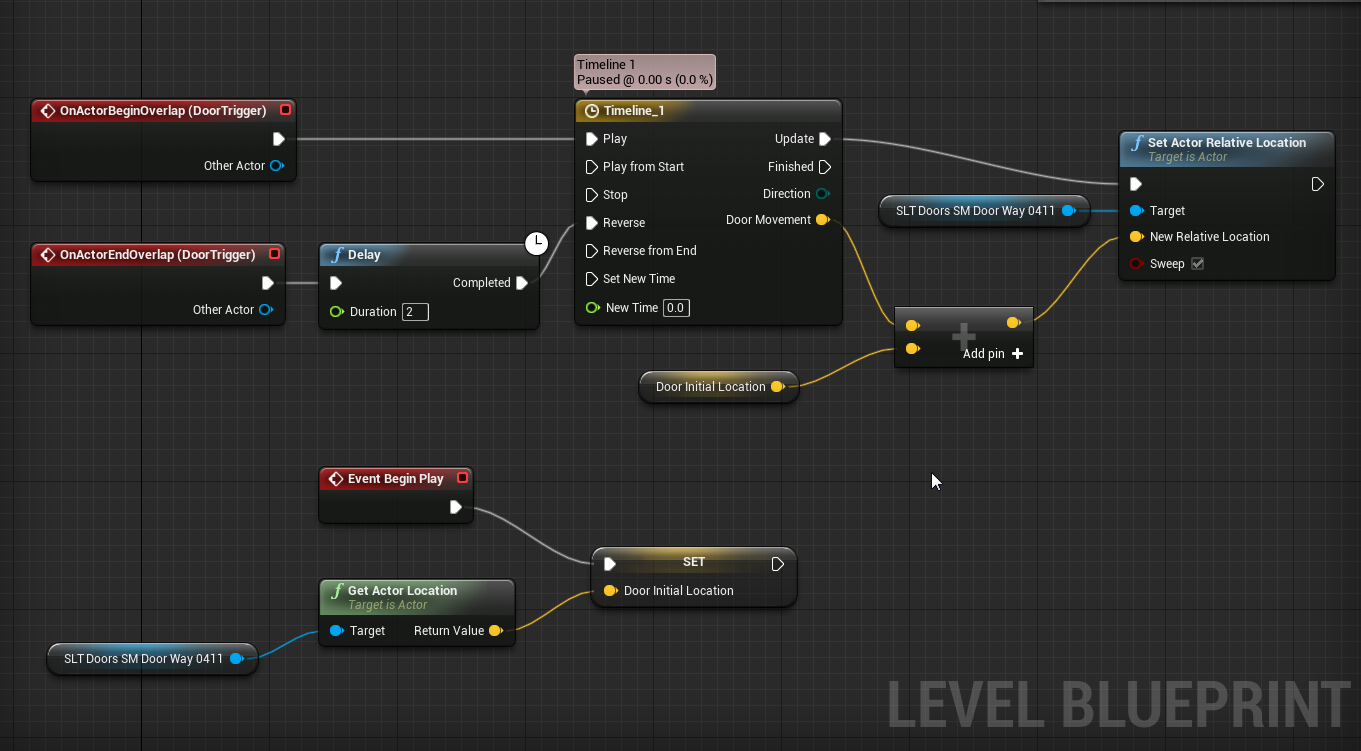
\includegraphics[width=0.9\textwidth]{OtherImages/UEBlueprint.png}
    \caption[BluePrints in Unreal Engine]{Blueprints in Unreal Engine allows users to drag and drop blocks rather than having to program.}
    \source{\url{https://docs.unrealengine.com/en-US/ProgrammingAndScripting/Blueprints/UserGuide/Timelines/Examples/OpeningDoors/index.html}}    \label{UnrealEngineBlueprint}
\end{figure}
\newpage
\begin{figure}[H]
    \centering
    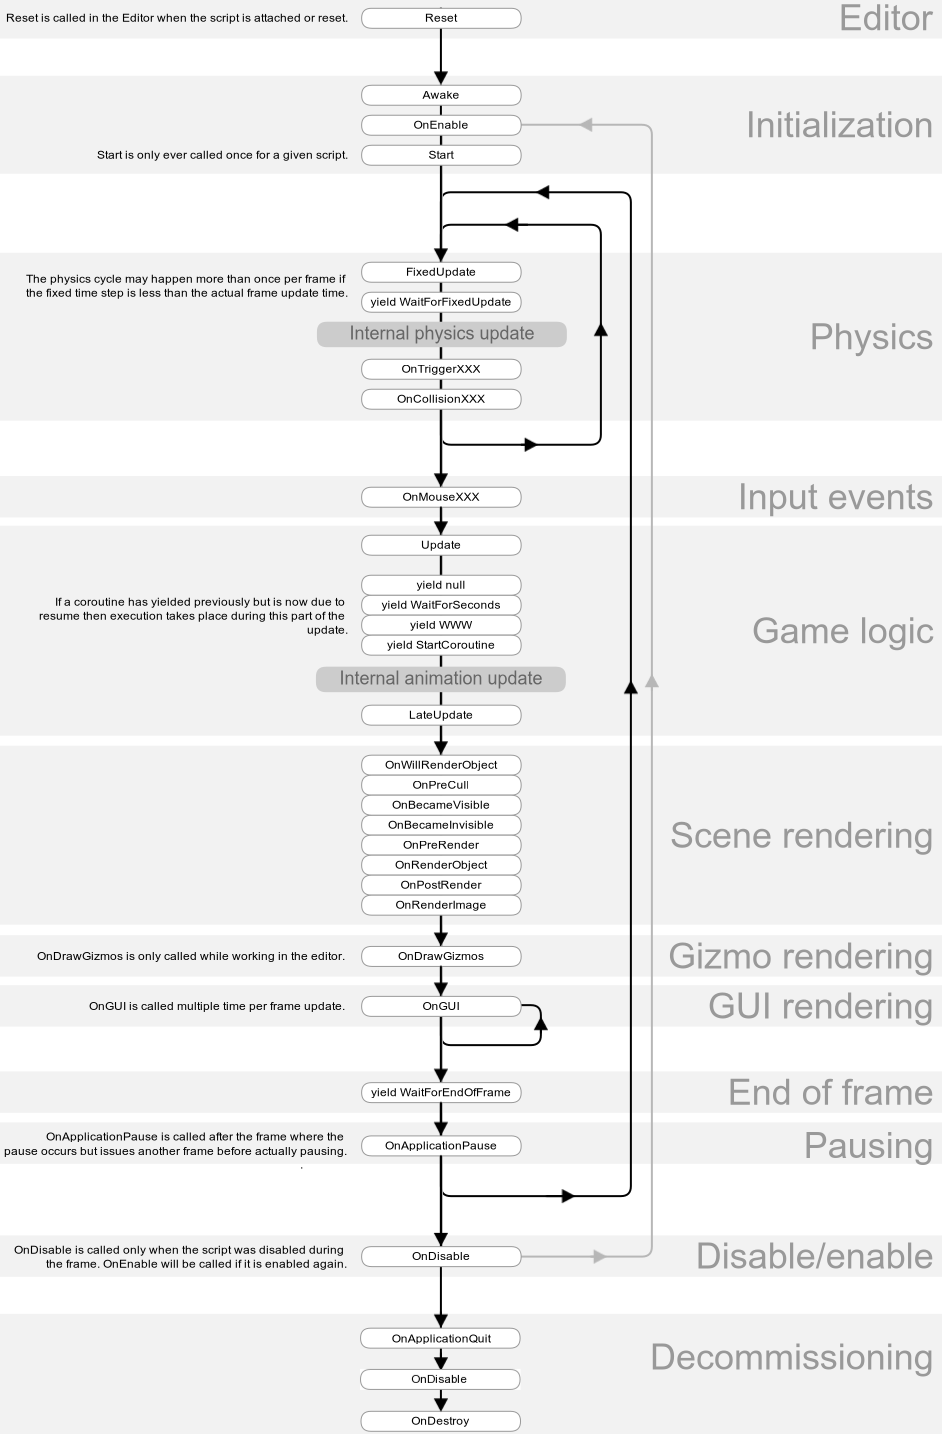
\includegraphics[width=0.95\textwidth]{03_Background/Appendix/Images/monobehaviour_flowchart.png}
    \caption[Monobehavior flow chart]{Flow chart of the actions in monobehavior. Fetched from Unity website.}
    \label{A:MonobehaviorFlow}
\end{figure}
\chapter[Indepth Simulator Research]{Simulator Research} \label{SimulatorResearch}
%%%%%%%% 4DV-Sim %%%%%%%%%%
\subsection{4DV-Sim}
\textbf{Description:} 4DV-Sim\footnote{Website: \url{https://www.4d-virtualiz.com/en/automotive-simulator}} is a simulator that is designed to emulate the hardware and sensors in autonomous systems. This is a professional product and has a variety of use cases from simulating farming to military equipment \cite{4dv-simulator}.

\textbf{Open Source:} No

\textbf{Operating System:} Linux

\textbf{Game Engine:} Non, but it does use PhysX for the physics engine

\textbf{Pros:} The simulator has a lot of available APIs. The simulator also comes with a configurable GUI to set up the simulation environment how you would like it. Also, as it is professionally made, it looks very good.   

\textbf{Cons:} It is not designed to train machine learning implementations on the simulator, but rather emulate a current hardware setup. Also, as it is not open source, it will not be something that we could modify or expand upon to suit our purposes. 

\textbf{Conclusion:} As 4DV-Sim is not an open-source product it is not something that we can use for this project. It is however interesting to see that simulators like this are needed not just for research purposes, but for customers who want to try out their hardware setup in an emulated environment.


\begin{figure}[H]
    \centering
    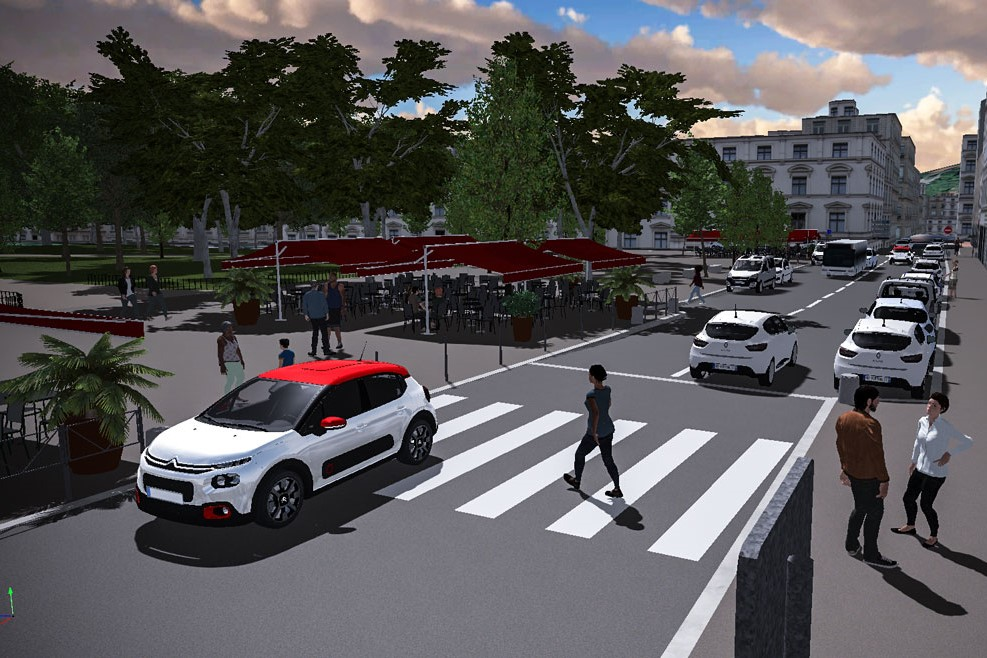
\includegraphics[width=0.5\textwidth]{03_Background/Appendix/Simulators/4DV-Sim.jpg}
    \caption{Source: \url{https://www.4d-virtualiz.com/en/automotive-simulator}}
\end{figure}

%%%%%%%% AirSIM %%%%%%%%%%
\subsection{AirSim} \label{AirSimDoc}
\textbf{Description:} AirSim\footnote{Website: \url{https://microsoft.github.io/AirSim}} is a simulator for cars and drones. It is open-source and works as a plugin for Unreal Engine, which means the simulator can be used with any environment which has been modeled inside the game engine. According to their website \cite{AirSim_Website}, the goal of the simulator is to create a platform for AI research to experiment with deep learning, computer vision, and reinforcement learning algorithms for autonomous systems. 

\textbf{Open Source:} Yes

\textbf{Operating System:} Any operating system

\textbf{Game Engine:} Primarily Unreal Engine, but it also offers a prototype version in Unity

\textbf{Pros:} Offers a large range of existing APIs. The simulator also has an active community on both discord and Github. It also gives the option to add drones. It is also designed to train machine learning models on it.

\textbf{Cons:} The simulator is not as realistic as other simulators. The vehicle physics is not as good as some of the other simulators, for example the handling and collisions. Also, currently, there are no pedestrians in the game. 

\textbf{Conclusion:} AirSim is worth looking closer into. As it is built using a game engine it should not be too hard to add the missing features, like for example adding and controlling pedestrians. In addition, as it is a plugin for Unreal Engine means that we can use other tools to import for example maps. Also, realistic vehicle physics was determined not to be an important factor for this project. 

\begin{figure}[H]
    \centering
    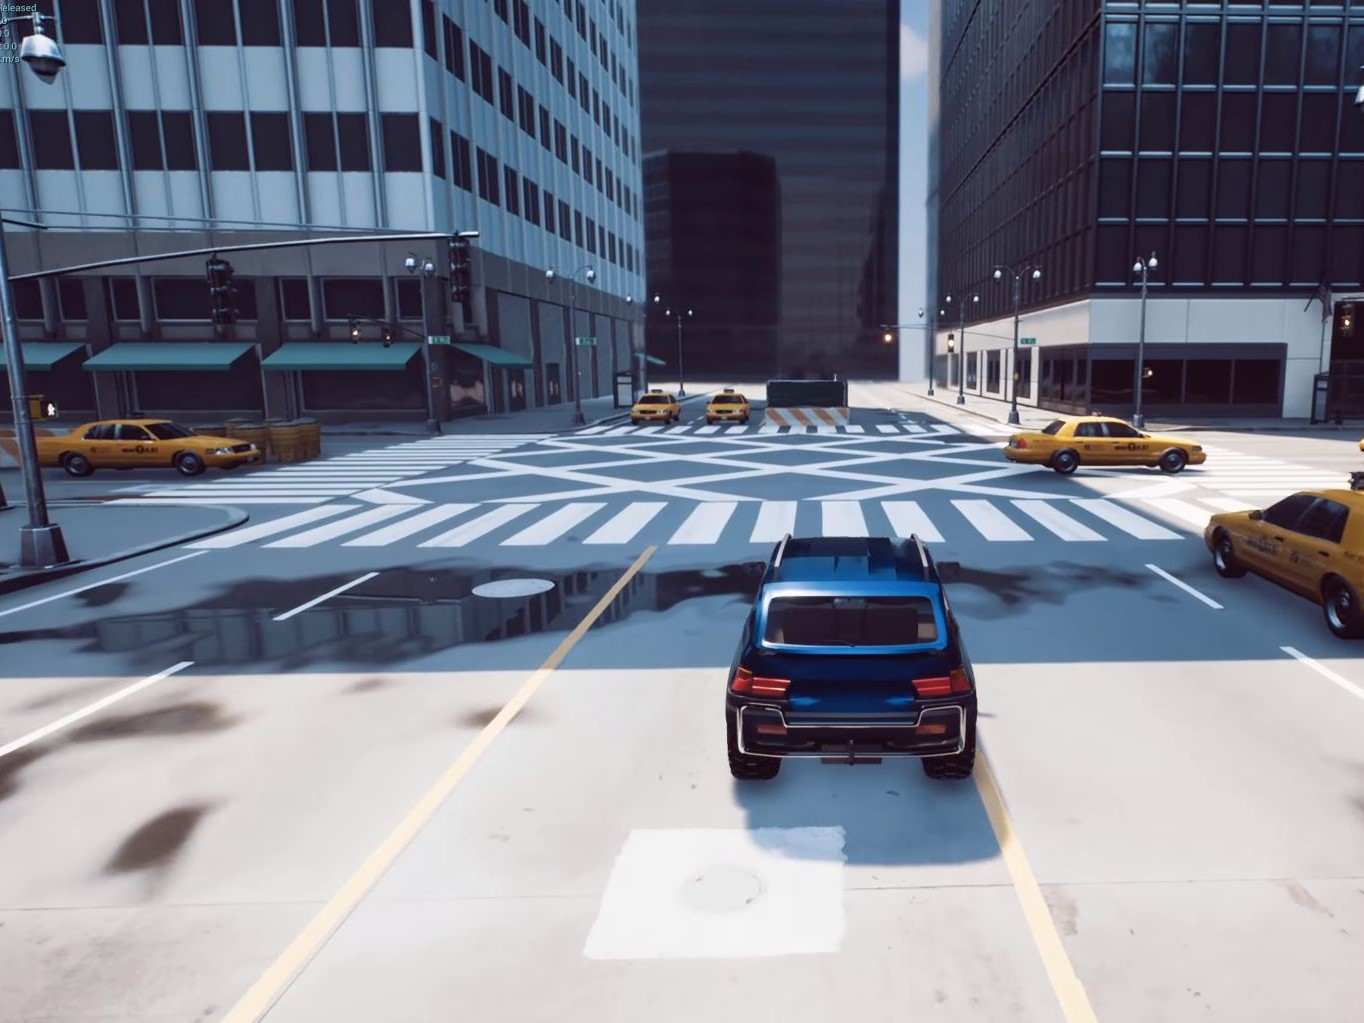
\includegraphics[width=0.5\textwidth]{03_Background/Appendix/Simulators/AirSim.JPG}
    \caption{Source: \url{https://microsoft.github.io/AirSim}}
\end{figure}

%%%%%%%% Apollo %%%%%%%%%%
\subsection{Apollo} \label{Apollo}
\textbf{Description:} Apollo\footnote{\url{https://github.com/ApolloAuto/apollo}} is a simulator that is designed to emulate the hardware in autonomous vehicles so that it can be trained for machine learning models. According to their website \cite{Apollo_Website}, Apollo is a flexible architecture that accelerates the development and testing of autonomous vehicles.

\textbf{Open Source:} Yes

\textbf{Operating System:} Any system that can run Docker

\textbf{Game Engine:} Unity

\textbf{Pros:} Accurately models the vehicle physics to help improve the machine learning model's accuracy. The simulator is also actively being worked on by a large community.  

\textbf{Cons:} It looks like quite a complex simulator, and it does therefore not seem like it will be easy to modify. The product is really specific towards training autonomous vehicles. 

\textbf{Conclusion:} Due to the complexity of this simulator, it does not look like something that we could build upon for this project. 

\begin{figure}[H]
    \centering
    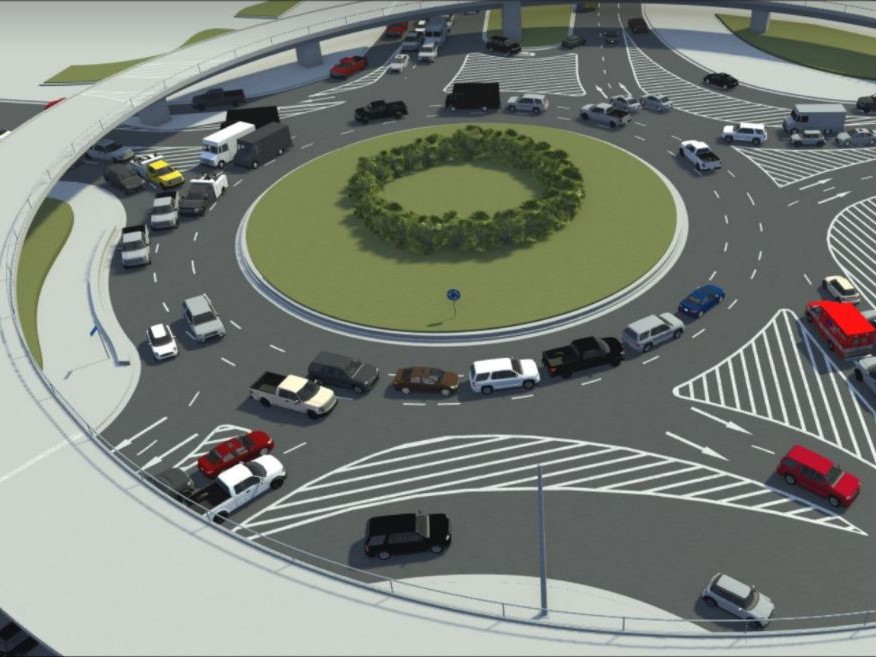
\includegraphics[width=0.5\textwidth]{03_Background/Appendix/Simulators/Apollo.JPG}
    \caption{Source: Slide deck from Apollo Game Engine Based Simulation Talk at GDC 2019 - \url{https://bit.ly/2VSzwlF}}
\end{figure}

%%%%%%%% Autoware %%%%%%%%%%
\subsection{Autoware} \label{Autoware}
\textbf{Description:} Autoware\footnote{\url{https://gitlab.com/autowarefoundation/autoware.auto/AutowareAuto}} is an open-source software for autonomous vehicles. It comes with a large variety of APIs  \cite{Autoware_doc_Website}. Autoware is however not a simulator, but can be used on a simulated vehicle to make it autonomous.

\textbf{Open Source:} Yes

\textbf{Operating System:} Robot Operating System (ROS)

\textbf{Game Engine:} Na

\textbf{Pros:} As it runs on ROS it can easily be adapted to work on a real autonomous vehicle.

\textbf{Cons:} Currently it only works with a specific car model and sensor set up. The software also seems quite complex, and combining it with a simulator will probably be quite challenging.

\textbf{Conclusion:} As this is not a simulator this is not something that we can use for this project. We will see with the LGSVL simulator (\ref{LGSVL_Simulator}), this software can be used alongside a simulator to model the autonomous system. 


%%%%%%%% Carla %%%%%%%%%%
\subsection{Carla} \label{Carla}
\textbf{Description:} Carla\footnote{\url{https://carla.org/}} is an open-source simulator for developing autonomous vehicles. It contains a variety of APIs and is actively being developed. Carla is also designed for training machine learning models \cite{CarlaPaper}. 

\textbf{Open Source:} Yes

\textbf{Operating System:} Primarily Linux, but also Windows

\textbf{Game Engine:} Unreal Engine

\textbf{Pros:} Has a lot of features already implemented, such as sensors, vehicle API, and the ability to add new objects. The simulator also has the ability to add pedestrians and plot their movement. Active community. Well documented and lots of information online. 

\textbf{Cons:} Difficult to add new and custom maps. Vehicle handling is not as realistic as some of the other simulators.

\textbf{Conclusion:} Carla is worth looking into further as it has most of the features that we are looking for.


\begin{figure}[H]
    \centering
    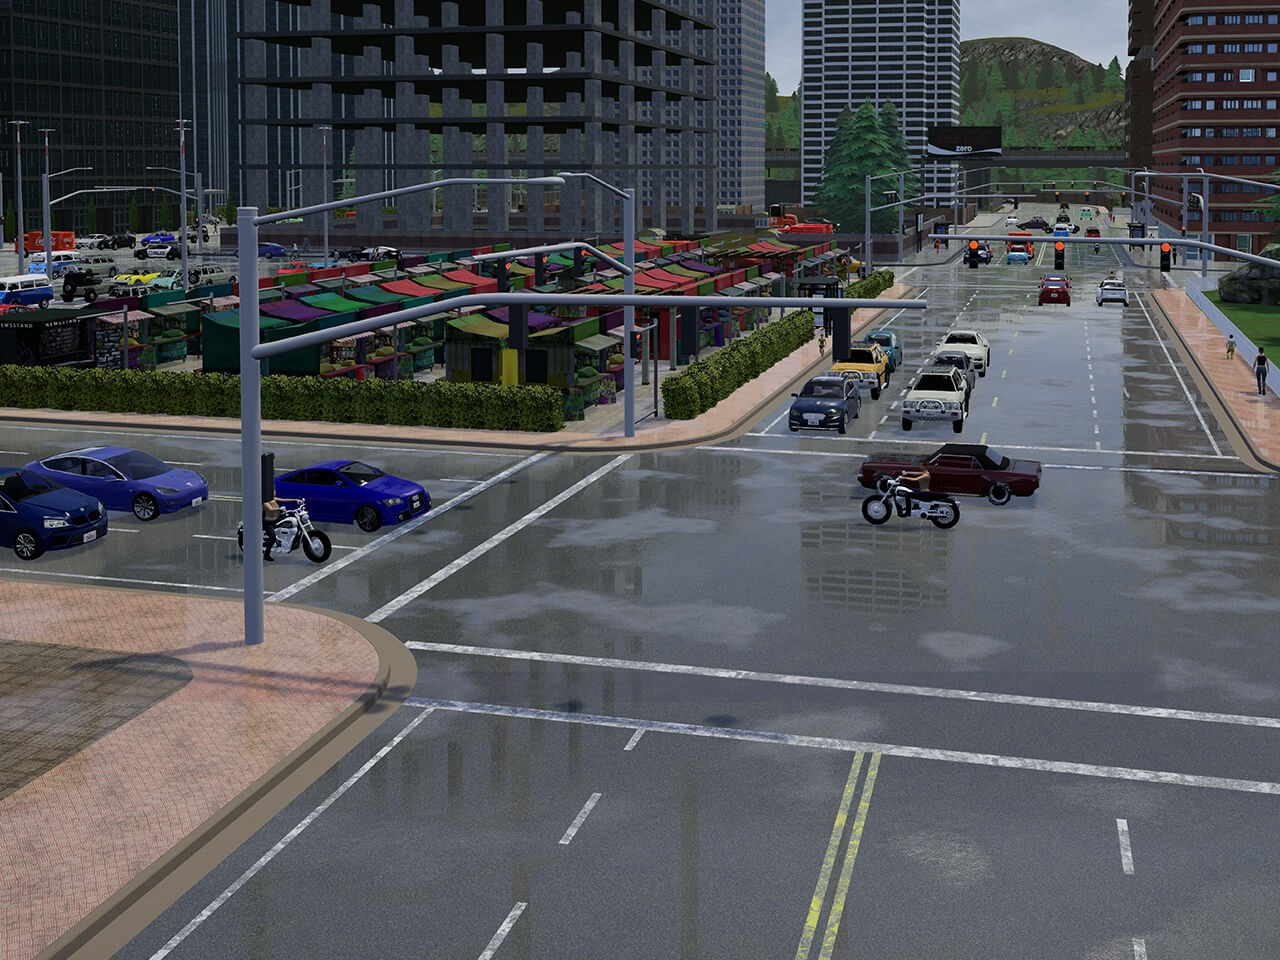
\includegraphics[width=0.5\textwidth]{03_Background/Appendix/Simulators/Carla.JPG}
    \caption{Source: \url{https://www.unrealengine.com/en-US/spotlights/carla-democratizes-autonomous-vehicle-r-d-with-free-open-source-simulator}}
\end{figure}


%%%%%%%% CrowdSim3D %%%%%%%%%%
\subsection{CrowdSim3D}
\textbf{Description:} CrowdSim3D\footnote{\url{https://crowdsim3d.com}} is primarily a simulator for modeling large crowds, but can also be used for vehicle traffic. 

\textbf{Open Source:} No (£180)

\textbf{Operating System:} Any operating system

\textbf{Game Engine:} Not specified

\textbf{Pros:} Has the ability to control several pedestrians and vehicles in a shared space.

\textbf{Cons:} Does not look to be designed for machine learning models. Difficult to add new models. Also, as it is not open source it will not be possible to customise the product. 

\textbf{Conclusion:} CrowdSim3D is not worth considering as we cannot adapt the product as it is not open source. 

\begin{figure}[H]
    \centering
    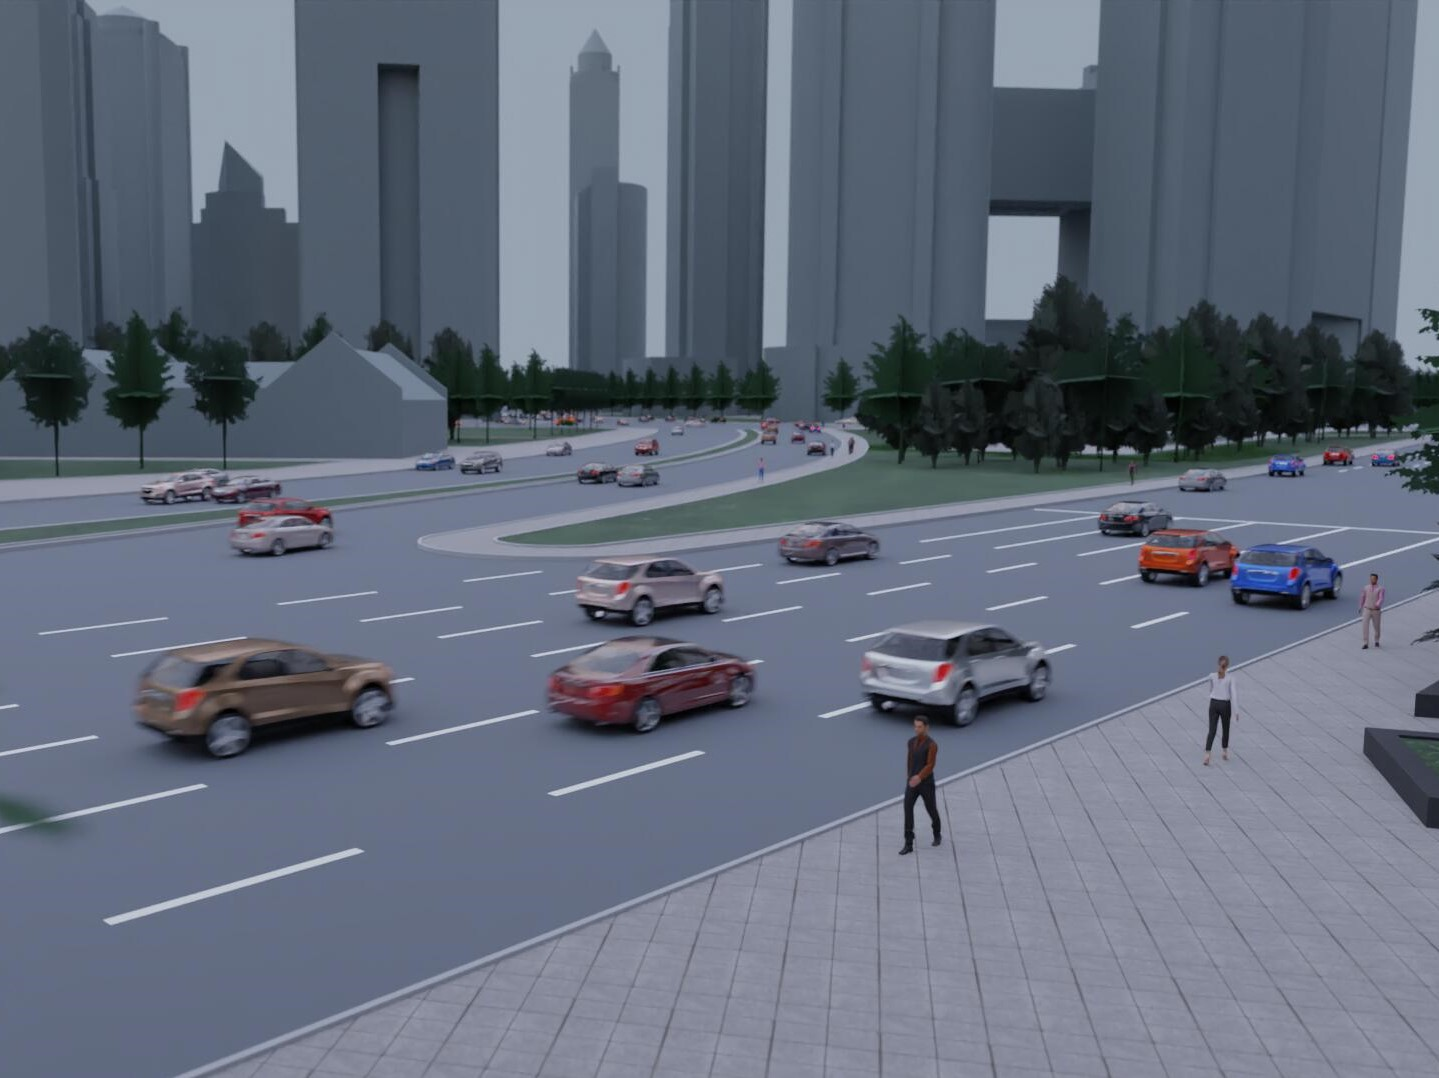
\includegraphics[width=0.5\textwidth]{03_Background/Appendix/Simulators/CrowdSim.JPG}
    \caption{Source: \url{https://crowdsim3d.com}}
\end{figure}


%%%%%%%% Deep Drive %%%%%%%%%%
\subsection{Deep Drive}
\textbf{Description:} Deep Drive\footnote{\url{https://deepdrive.voyage.auto/}} is an open-source simulator aimed to train neural networks for self-driving cars \cite{DeepDrive_Website}. They also provide you with a large data set to train your autonomous vehicle on. 

\textbf{Open Source:} yes

\textbf{Operating System:} Any operating system

\textbf{Game Engine:} Unreal Engine

\textbf{Pros:} Is able to handle a variety of different sensors and vehicle setups. It also has an active community and a leader board where you can compare your trained neural network against other developers. 

\textbf{Cons:} Currently there are three maps available, but it is not easy to add your own maps. Also, it is not designed to be customised. Currently, there are no pedestrians and no APIs.

\textbf{Conclusion:} Deep Drive is not a simulator that is worth looking at as it is not designed to be customised. It also lacks most of the features we are looking for. 

\begin{figure}[H]
    \centering
    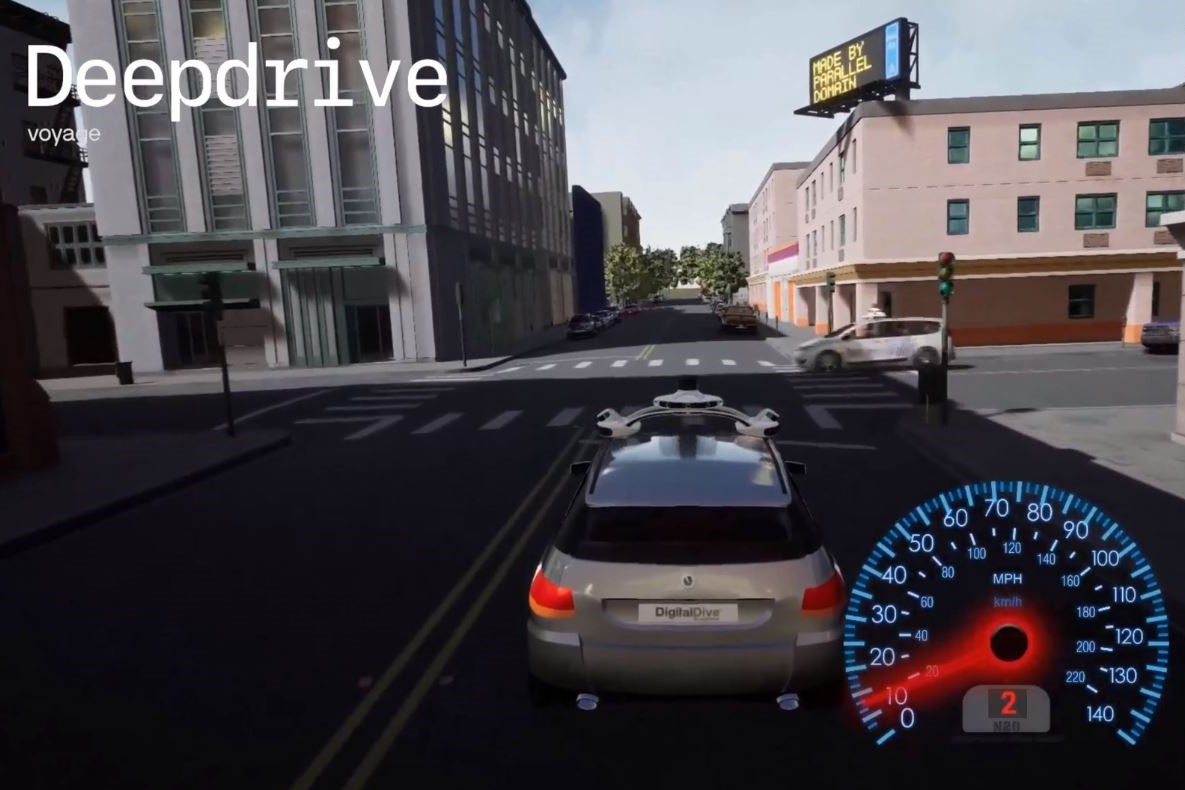
\includegraphics[width=0.5\textwidth]{03_Background/Appendix/Simulators/DeepDrive.JPG}
    \caption{Source: \url{https://deepdrive.voyage.auto}}
\end{figure}

%%%%%%%% Donkey Car Simulator %%%%%%%%%%
\subsection{Donkey Car Simulator}
\textbf{Description:} Donkey Car Simulator\footnote{\url{https://docs.donkeycar.com/guide/simulator}} is a simulator for the Donkey Car. The car itself costs roughly £200 and can be ordered online, or you can download the schematics for free. The simulator can be used to train a neural network in Python which can then run on your car. 

\textbf{Open Source:} Yes

\textbf{Operating System:} Any operating system

\textbf{Game Engine:} Unity

\textbf{Pros:} Easy to use

\textbf{Cons:} Not what we are looking for as it is only used to train a real toy car.

\textbf{Conclusion:} Donkey Car is an interesting project to read about as it is a fun kit that introduces people to autonomous cars. However, it is not what we are looking for for this project as the simulator is not customisable and there is only one vehicle. 


\begin{figure}[H]
    \centering
    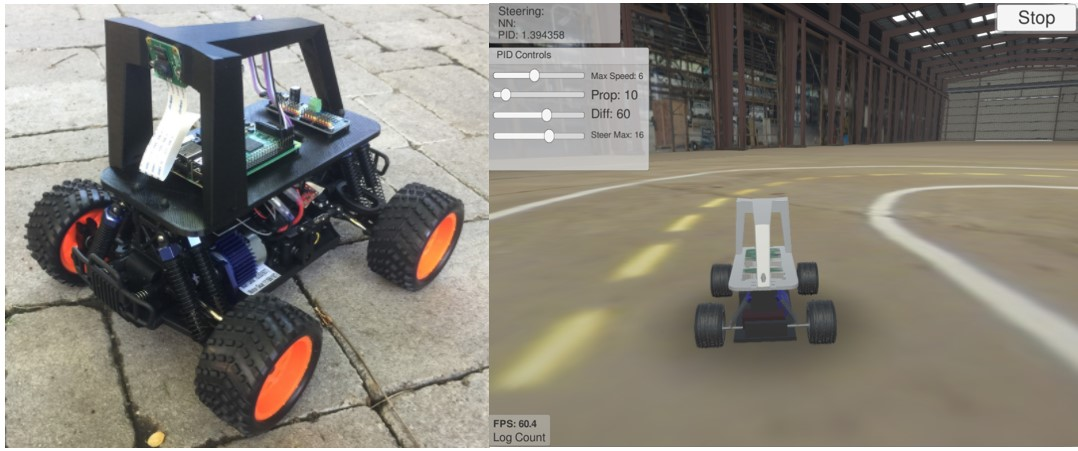
\includegraphics[width=0.5\textwidth]{03_Background/Appendix/Simulators/DonkeySim.jpg}
    \caption{Source: \url{https://docs.donkeycar.com}}
\end{figure}

%%%%%%%% Gazebo %%%%%%%%%%
\subsection{Gazebo}\label{gazebo}
\textbf{Description:} Gazebo\footnote{\url{http://gazebosim.org}} is a robotics simulator designed to design robots, test algorithms and train AI systems \cite{Gazebo_Website}. Gazebo offers the ability to simulate several robots at once in both indoor and outdoor environments.

\textbf{Open Source:} Yes

\textbf{Operating System:} Any operating system

\textbf{Game Engine:} ODE, but also Bullet, Simbody and DART which are additional physics engines. 

\textbf{Pros:} Very versatile, can be used for much more than traffic simulations. 

\textbf{Cons:} Due to the large number of different physics engines it might be complicated to fix something if a feature breaks. The documentations is not as clear as some other simulators. 

\textbf{Conclusion:} Gazebo is worth looking at as it is widely used for robotics simulations. All the sensing APIs are already implemented.


\begin{figure}[H]
    \centering
    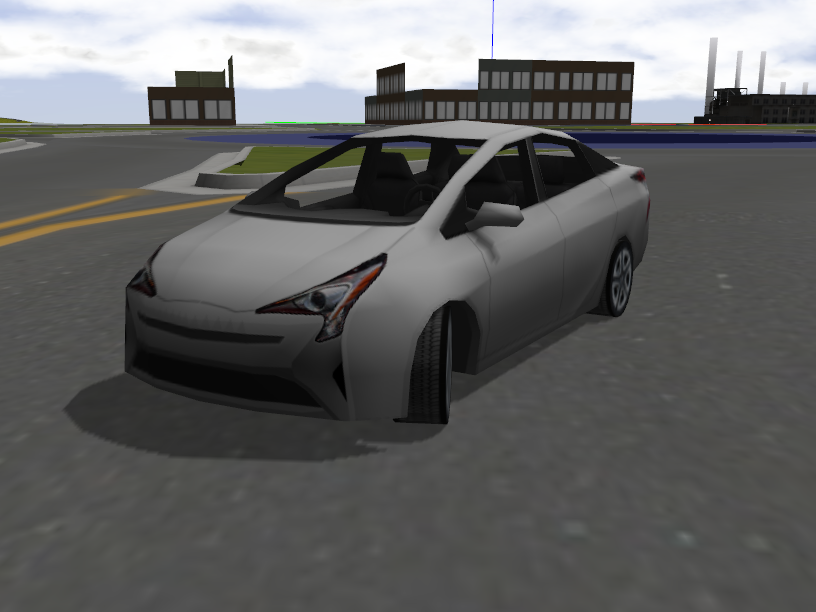
\includegraphics[width=0.5\textwidth]{03_Background/Appendix/Simulators/gazebo.png}
    \caption{Source: \url{http://gazebosim.org/blog/vehicle\%20simulation}}
\end{figure}


%%%%%%%% LPZRobots %%%%%%%%%%
\subsection{LPZRobots}
\textbf{Description:} LPZRobots\footnote{\url{https://github.com/georgmartius/lpzrobots}} is a robotics simulator created by the Robotics Group for Self-Organisation of Control at the University of Leipzig in Germany \cite{LPZRobots_Website, LPZRobots_book}. The simulator aims to have an open environment to simulate the robot's physics. 

\textbf{Open Source:} Yes

\textbf{Operating System:} Primarily Linux, but now also supports Windows

\textbf{Game Engine:} ODE

\textbf{Pros:} Free to add any kind of robot.

\textbf{Cons:} The code has not been updated since 2018 and the last release was in 2016. Unlike other simulators, this one does not seem to have an active community. 

\textbf{Conclusion:} As the development of the LPZRobots simulator has been inactive for several years, makes it not worth considering. The simulator also lacks most of the features we are looking for. 

\begin{figure}[H]
    \centering
    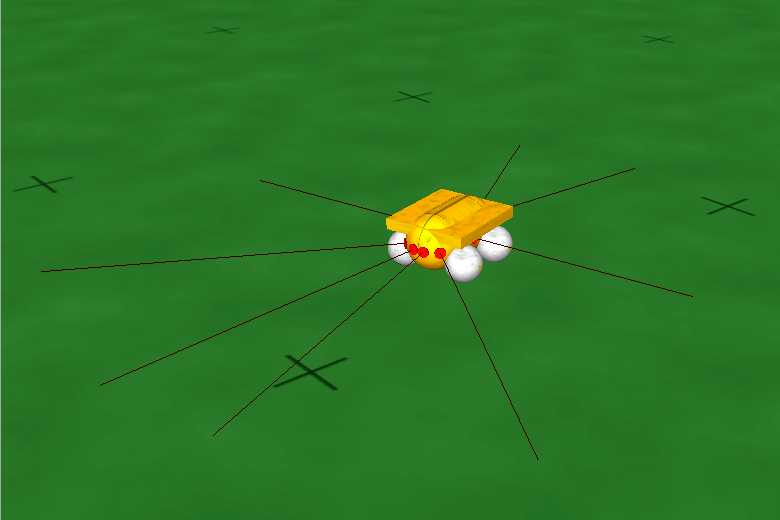
\includegraphics[width=0.5\textwidth]{03_Background/Appendix/Simulators/LPZRobots.png}
    \caption{Source: \url{https://itp.uni-frankfurt.de/~gros/StudentProjects/Robots\_2016\_ObstacleAvoidance}}
\end{figure}


%%%%%%%% LGSVL Simulator %%%%%%%%%%
\subsection{LGSVL Simulator} \label{LGSVL_Simulator}
\textbf{Description:} LGSVL\footnote{\url{https://github.com/lgsvl/simulator}} is a simulator created by the Advanced Platform Lab at the LG Electronics America R\&D Center \cite{LGSVL_Web}. The simulator combines the vehicle from Autoware (Section~\ref{Autoware}) with Apollo (Section~\ref{Apollo}) which emulates the hardware. The LGSVL has lots of available APIs such as cameras, LiDAR, RADAR, and GPS. Some environmental parameters can also be changed such as the map, weather, and pedestrians.
% Uses Apollo and Autoware

\textbf{Open Source:} Yes

\textbf{Operating System:} Windows 10

\textbf{Game Engine:} A variety due to its complexness, but both Unreal Engine and Unity.

\textbf{Pros:} Has most of the features we are looking for.

\textbf{Cons:} Relies on a lot of different components. The codebase is therefore large and complex and it looks difficult to add our own features such as our own entity.

\textbf{Conclusion:} The LGSVL Simulator would probably not work for us as the code-base seems too large and complex.

\begin{figure}[H]
    \centering
    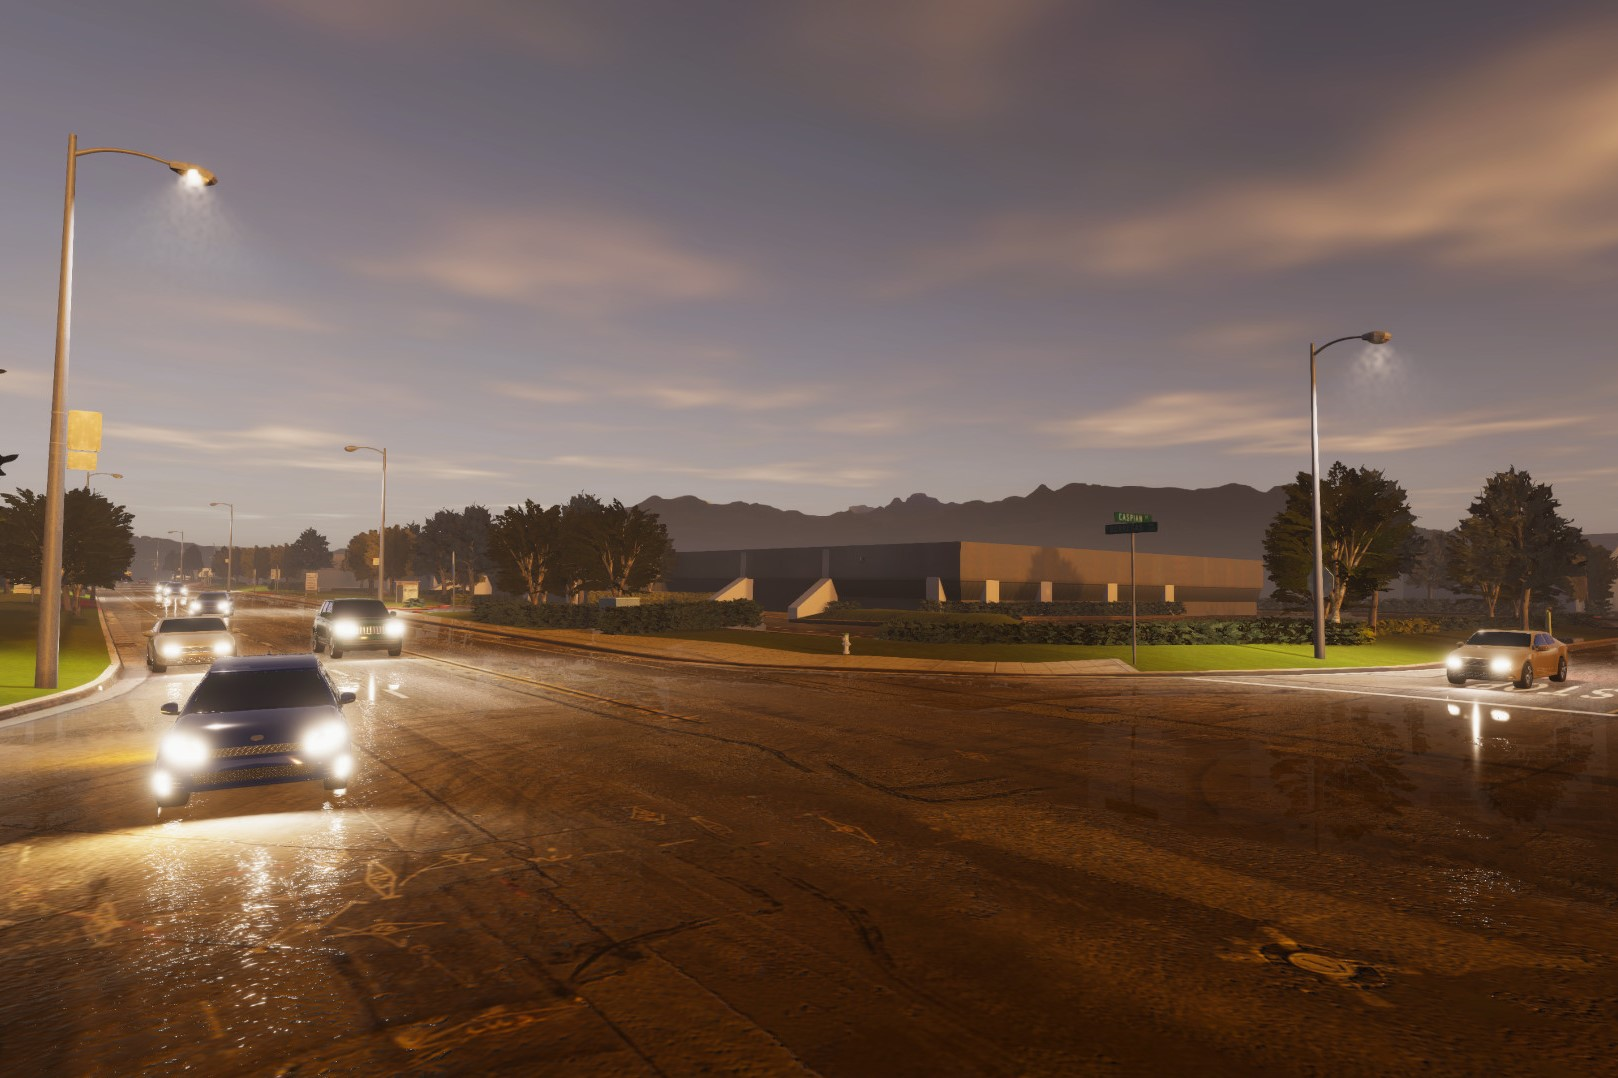
\includegraphics[width=0.5\textwidth]{03_Background/Appendix/Simulators/LGSVL.jpg}
    \caption{Source: \url{https://www.lgsvlsimulator.com/about}}
\end{figure}
%https://github.com/lgsvl/simulator

%%%%%%%% Marilou %%%%%%%%%%
\subsection{Marilou}
\textbf{Description:} Marilou\footnote{\url{http://www.anykode.com/index.php}} is a simulator created by ANYKODE \cite{Marilou_Web}. Marilou is an open map simulator where the user can add objects and hindrances for the robot to navigate around. The simulator is designed to simulate simultaneous localisation and mapping (SLAM) and other localisation techniques. 

\textbf{Open Source:} No (£350)

\textbf{Operating System:} Windows and Linux

\textbf{Game Engine:} Unknown

\textbf{Pros:} Accurately simulates sensors and robot behavior. Easy to add new objects and other controllable entities. 

\textbf{Cons:} As the simulator is not open source, we cannot modify its behavior. Latest release 2018.

\textbf{Conclusion:} Marilou is not a simulator that we can use for this project as it is not open source. In addition, it is not designed with APIs in mind and controlling multiple objects at once looks impossible in the current program. 

\begin{figure}[H]
    \centering
    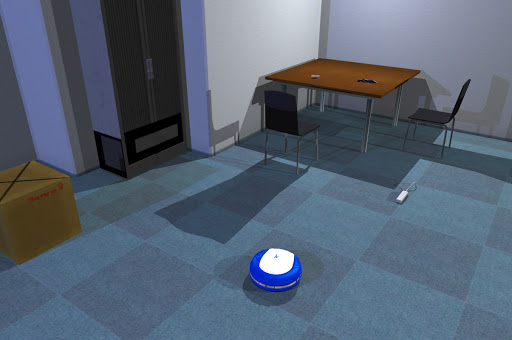
\includegraphics[width=0.5\textwidth]{03_Background/Appendix/Simulators/Marilou.jpg}
    \caption{Source: \url{http://www.anykode.com/downloads.php}}
\end{figure}


%%%%%%%% rFpro %%%%%%%%%%
\subsection{rFpro}
\textbf{Description:} rFpro\footnote{\url{https://www.rfpro.com}} is a driving simulation software which focuses on road-vehicle simulation \cite{rFpro_Web}. rFpro allows for a variety of use cases, from training machine learning models for autonomous driving \cite{rFpro_ML}, to motor racing.

\textbf{Open Source:} No

\textbf{Operating System:} Windows

\textbf{Game Engine:} ISIMotor - A game engine created by Image Space Inc \cite{ISIMotor}. The game engine is used for F1 and other racing games.

\textbf{Pros:} A professionally made simulator that has most of the features we are looking for. Very good graphics and accurate vehicle behavior. 

\textbf{Cons:} rFpro does not give us access to any of the source code. The price is only available upon request, but it is most likely too expensive for this project. 

\textbf{Conclusion:} Even though rFpro contains just about all of the features we are looking for, and is probably the best-looking simulator, it will not work for this project as it is not open source. 

\begin{figure}[H]
    \centering
    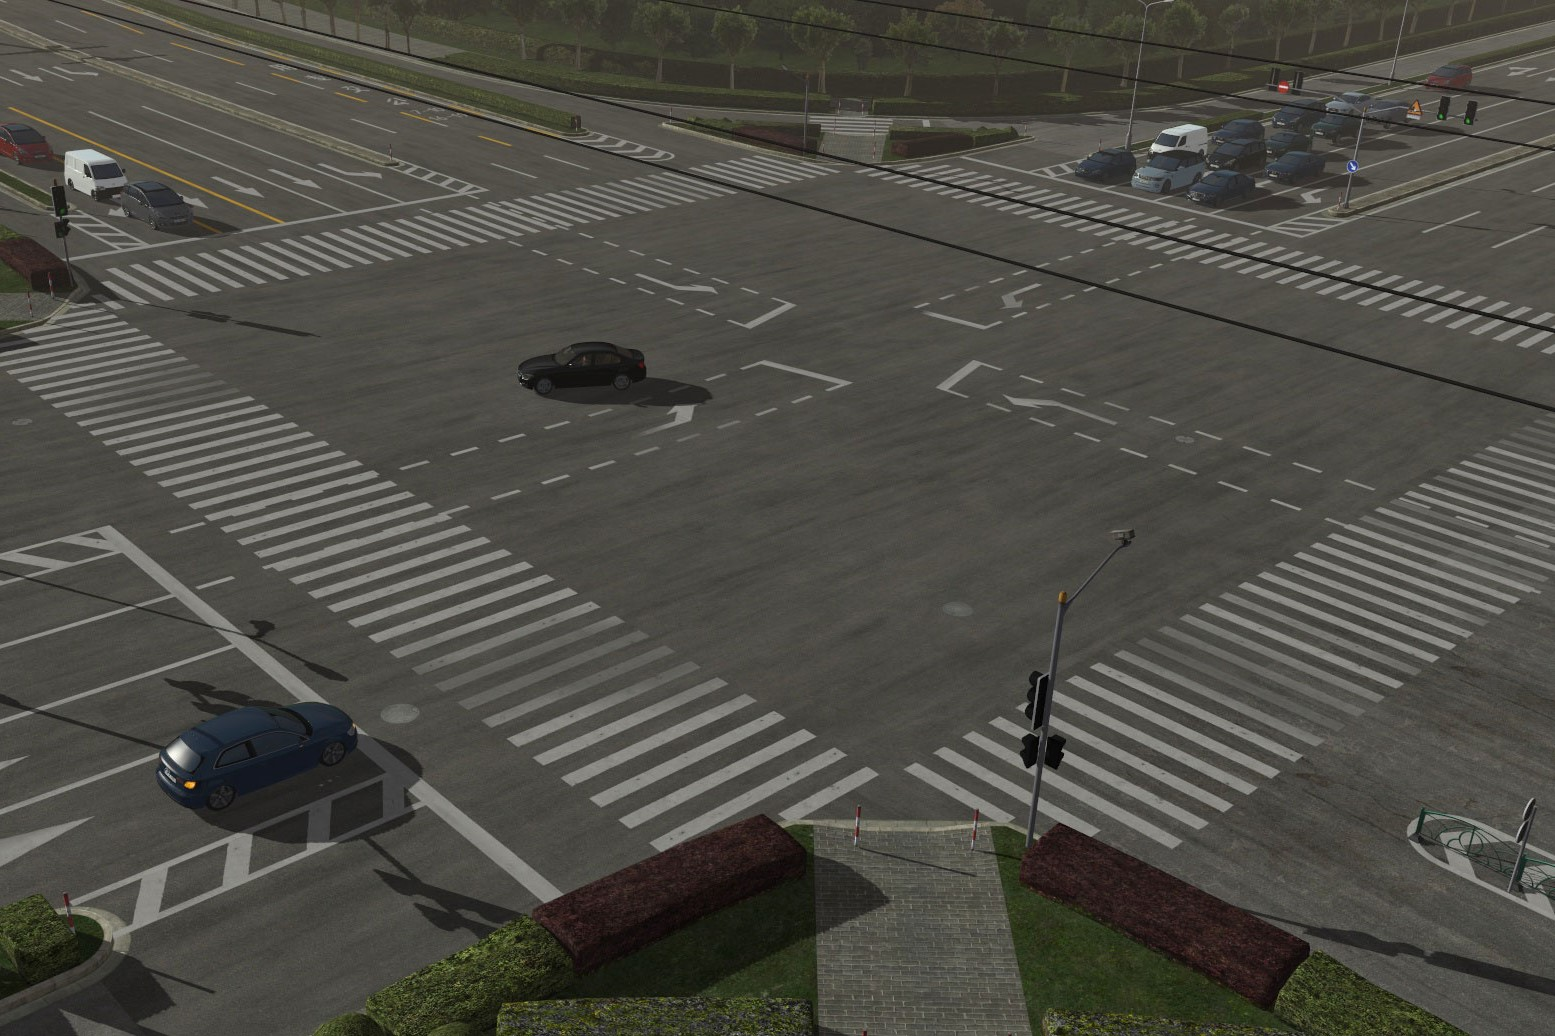
\includegraphics[width=0.5\textwidth]{03_Background/Appendix/Simulators/rFpro.jpg}
    \caption{Source: \url{http:https://www.rfpro.com/driving-simulation}}
\end{figure}

%%%%%%%% Rigs of Rods %%%%%%%%%%
\subsection{Rigs of Rods}
\textbf{Description:} Rigs of Rods\footnote{\url{https://www.rigsofrods.org}} (RoR) is an open-source physics simulator primarily designed to simulate vehicle physics. The simulator uses soft-body physics which means that if the vehicle collides, its structure will be deformed. This will result in a more accurate simulation.

\textbf{Open Source:} Yes

\textbf{Operating System:} Windows and Linux

\textbf{Game Engine:} Non, creates its own soft-body physics engine.

\textbf{Pros:} There is an active community creating modifications for the simulator. Also, the only simulator on the list which uses soft-body physics. 

\textbf{Cons:} There are no APIs currently available. 

\textbf{Conclusion:} As for this project, we are not looking for realistic features, but rather certain APIs. This simulator will require too much work to add the missing features. It is therefore not a simulator that is worth considering. 

\begin{figure}[H]
    \centering
    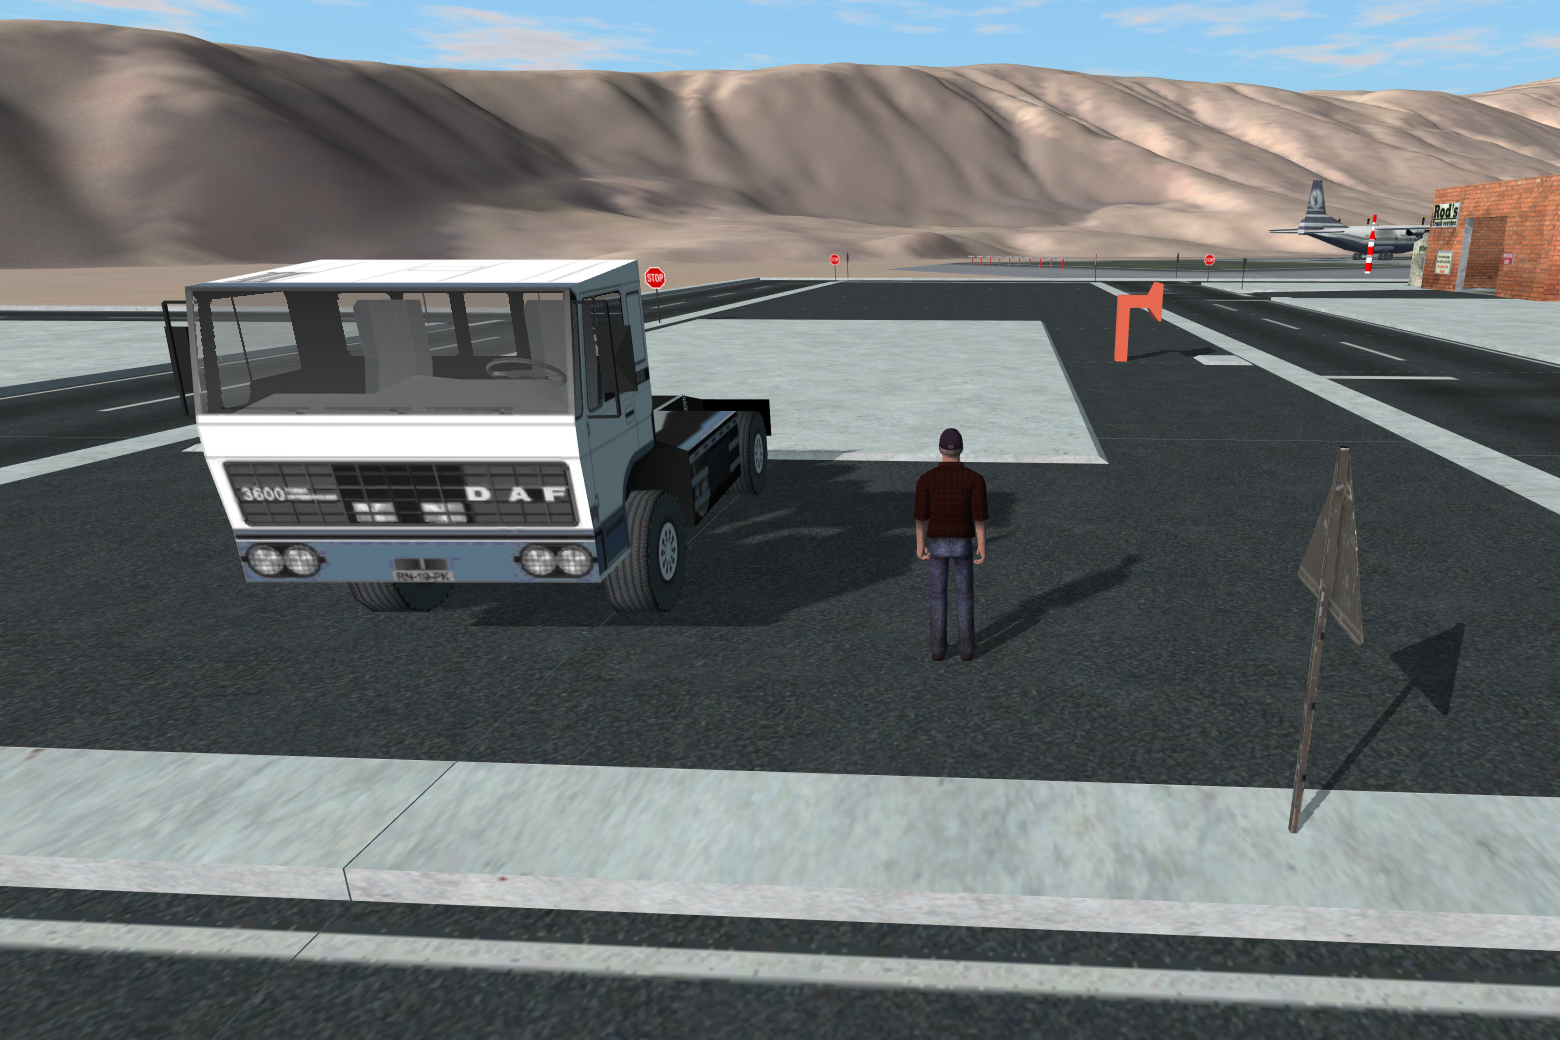
\includegraphics[width=0.5\textwidth]{03_Background/Appendix/Simulators/RoR.png}
    \caption{Source: \url{https://docs.rigsofrods.org/gameplay/beginners-guide}}
\end{figure}


%%%%%%%% TORCS - The Open Racing Car Simulator %%%%%%%%%%
\subsection{TORCS - The Open Racing Car Simulator}
\textbf{Description:} TORCS\footnote{\url{https://sourceforge.net/projects/torcs}} is an open-source racing car simulator. It can be used as an ordinary racing game or as an AI racing research platform. The creators of TORCS used to host competitions on its website among players for who could create the best artificially intelligent racing car \cite{TORCS_Racing}. 

\textbf{Open Source:} Yes

\textbf{Operating System:} Linux and Windows

\textbf{Game Engine:} Non, implemented from scratch.

\textbf{Pros:} Easy to add and create new content. 

\textbf{Cons:} Latest release 2016 but mainly developed in 2008. Also, has no available APIs and no pedestrians.

\textbf{Conclusion:} This simulator is lacking most of the features we are looking for. It is also quite outdated. TORCS is therefore not worth considering. 

\begin{figure}[H]
    \centering
    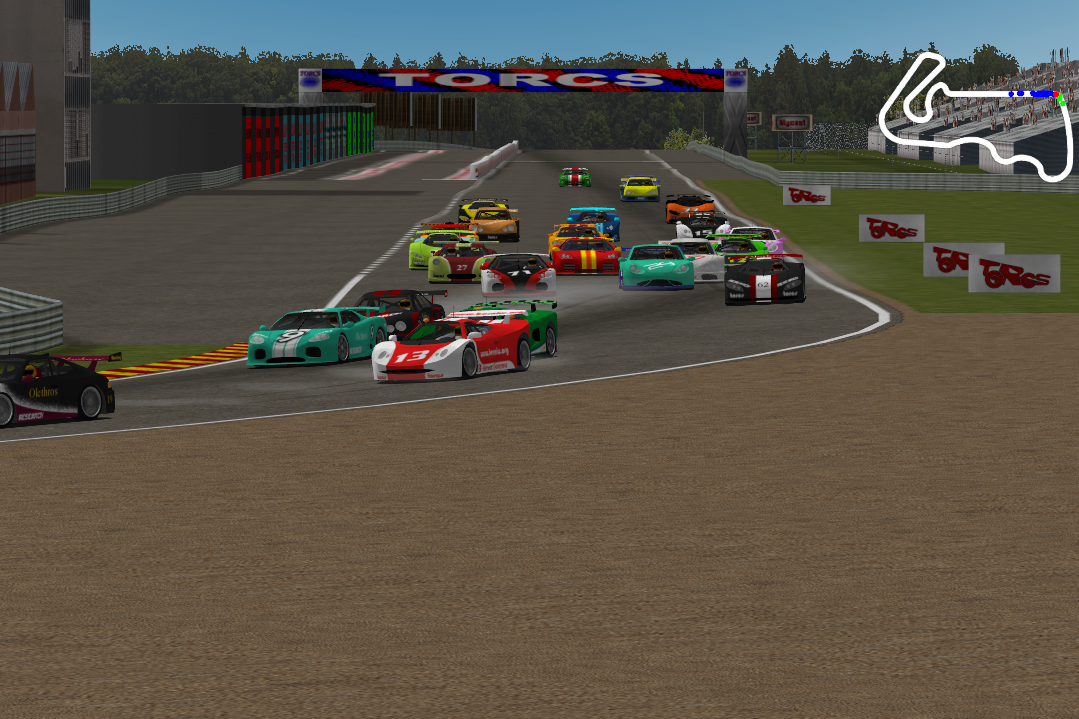
\includegraphics[width=0.5\textwidth]{03_Background/Appendix/Simulators/TORCS.png}
    \caption{Source: \url{https://sourceforge.net/projects/torcs}}
\end{figure}

%%%%%%%% Webots %%%%%%%%%%
\subsection{Webots}
\textbf{Description:} Webots\footnote{\url{https://www.cyberbotics.com}} is an open-source robotics simulator developed by Cyberbotics \cite{Webots_Github}. Webots provides a complete developing environment to model, program and simulate the robots \cite{Webots_home}. 

\textbf{Open Source:} Yes

\textbf{Operating System:} Any operating system

\textbf{Game Engine:} ODE

\textbf{Pros:} A lot of documentation on how to add new features. Seems to be able to generate new maps easily. Available chat page.

\textbf{Cons:} There does not seem to be many APIs to control multiple entities. All the APIs are mainly used for sensing. 

\textbf{Conclusion:} Webots has most of the features that we are looking for, however seems to lack the ability to easily control multiple entities at once. The simulator also seems less advanced than Gazebo (Section~\ref{gazebo}), so as an open area robotics simulator, we will rather look at that one first. We will therefore not be considering Webots.

\begin{figure}[H]
    \centering
    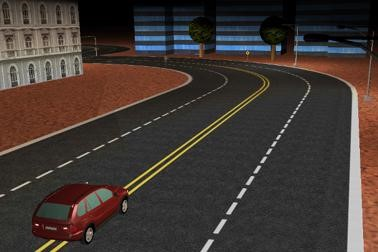
\includegraphics[width=0.5\textwidth]{03_Background/Appendix/Simulators/Webots.jpg}
    \caption{Source: \url{https://www.cyberbotics.com/doc/automobile/city-night}}
\end{figure}

\subsection{Conclusion}
After looking at the different simulators we decided to look further into AirSim (Section~\ref{AirSimDoc}), Carla (Section~\ref{Carla}) and Gazebo (Section~\ref{gazebo}). These are the simulators that will hopefully be the easiest to adapt and modify to suit our needs. In the next section, Analysis of Competing Product (Section~\ref{AoCP}), we will look at which of these three simulators to go for. 
%https://www.hisour.com/robotics-simulator-42971/


\chapter{Ethical, Legal and Safety Considerations}
\section{Ethical Considerations}
As this is just a simulation, there are not really any ethical concerns as such. 
\\~\\
If we however decide to look use the knowledge we learn in our simulator on a physical system there are a few things worth thinking about. Ethical considerations for autonomous systems have been a discussion for a long time \cite{ArkinRonaldC2016EaAS, BorensteinJason2019SCaE}. There are a variety of different ethical concerns. To name just a few, will an autonomous system be responsible enough \cite{BorensteinJason2019SCaE}, who would be responsible for an accident involving a self-driving car, and how could autonomous vehicles impact peoples behavior \cite{moralComputers}. These are not ethical concerns for the project as is, but could become an issue once we decide what the plan for the future is (Section~\ref{FuturePlanning}). 

\section{Legal Considerations}
AirSim has an MIT license which means that we can use the simulator however we like \cite{MITLicense}. This is the same license that is used for StreetMap. In regards to the game engine, as we have chosen to use AirSim which uses Unreal Engine, we are free to distribute the simulator as long as we don't make a gross profit of more than \$1 million \cite{UE5}. 
\\~\\
It could also be worth considering what the UK rules for autonomous vehicles are\footnote{\url{https://assets.publishing.service.gov.uk/government/uploads/system/uploads/attachment_data/file/929352/innovation-is-great-connected-and-automated-vehicles-booklet.pdf}}, if in the future work we decide to introduce a physical system \cite{UKAutoRules, UKAutoRulesGov2}. 


\section{Safety Considerations}
In regards to the project itself, there are no safety issues as it is a simulator being worked on from home. 
\\~\\
As mentioned in the other two sections. If information from the simulator ever gets used in a physical product there are a few things worth considering. Firstly, it is important to remember these are only simulations. Training a machine learning model on the simulator will not accurately reflect the behavior in real life. Secondly, it is important when testing a physical system that it does not for example collide with someone. This could be prevented by driving slowly or not driving where other people or objects might be in the way.

\chapter{User Guide} \label{UserGuide}
\section{Code Overview}
\paragraph{Added Files}

\paragraph{Updated Files}


\section{Simulator Research}
In this section we will look at a large variety of different simulators, to determine which one best suits our purpose. We will be looking at which operating system and game engine the simulator uses, whether or not it is open source, and the pros and cons of each simulator. We will be particularly looking at the simulators sensing abilities, ability to add additional entities, map customisability, available APIs, and how user-friendly the simulator is. Aspects of the simulator which is not as important as how realistic the simulator physics is, and how visually good looking it is. These are criteria formed by the project specification (Section~\ref{ProjectSpec})
\\~\\
The purpose of this section is to get a good understanding of the different simulators currently in existence.

\subsection{Overview}

% \usepackage{tablefootnote}
% \usepackage{array}
% \usepackage{pdflscape}
% \usepackage{longtable}


% \usepackage{tablefootnote}
% \usepackage{array}
% \usepackage{pdflscape}
% \usepackage{longtable}

\begin{landscape}
% \usepackage{tablefootnote}
% \usepackage{array}
% \usepackage{rotating}
\begin{table}
\resizebox{\columnwidth}{!}{%
\begin{tabular}{lllllllllll}
\textbf{Simulator~ ~ ~ ~ ~} & \textbf{\thead[l]{Open\\Source}} & \textbf{OS}\tablefootnote{"Any" means most commonly used Linux distributions, Windows and MAC} & \textbf{Game Engine} & \textbf{Development}\tablefootnote{"Actively Developed" means that there were several releases in the past year} & \textbf{Support} & \textbf{Pedestrians} & \textbf{Extensibility} & \textbf{\thead[l]{Multiple\\Agents}} & \textbf{Existing APIs} & \textbf{\thead[l]{Worth\\Considering}\tablefootnote{Reasoning for the decision can be found in the Appendix \ref{Appendix}}} \\
4DV-Sim & No & Linux & \thead[l]{PhysX\\(Physics Engine)} & \thead[l]{Actively\\ Developed} & Company offers support & Yes & No & Yes & Yes & No \\
AirSim & Yes & Any & \thead[l]{Primarily UE4,\\ but also Unity} & \thead[l]{Actively\\ Developed} & GitHub Issues & No & Yes & Yes\tablefootnote{Multiple agents is possible, but in a very limited number and has to be declared at the start.} & Yes & Yes \\
Apollo & Yes & Docker & Unity & \thead[l]{Actively\\ Developed} & GitHub Issues & No & Difficult & No & No & No \\
Autoware & Yes & ROS & N/A & \thead[l]{Actively\\ Developed} & GitLab Issues & No & Difficult & No & Limited\tablefootnote{\label{Footnote:03_Background:SimulatorResearchLimited}No sensing APIs} & No \\
Carla & Yes & Linux\tablefootnote{Linux is the main platform and they are aiming to support Windows as well. Currently Carla does not work on Windows.} & UE4 & \thead[l]{Actively\\ Developed} & GitHub Issues & Yes & Yes & Yes & Yes & Yes \\
CoppeliaSim & Yes\tablefootnote{More information can be found here: \url{https://www.coppeliarobotics.com/helpFiles/en/licensing.htm}} & Any & \thead[l]{Several different \\ physics engines} & \thead[l]{Actively\\ Developed} & Forum\tablefootnote{\url{https://forum.coppeliarobotics.com/}} & Yes & Difficult & Yes & Yes & No \\
CrowdSim3D & No & Any & N/A & Unknown & Company offers support & Yes & No & Yes & Yes & No \\
Deep Drive & Yes & Any & UE4 & \thead[l]{Last Commit\\ June 2020} & GitHub Issues & No & Yes & Yes & No & No \\
\thead[l]{Donkey Car\\ Simulator} & Yes & Any & Unity & \thead[l]{Actively\\ Developed} & GitHub Issues & No & Yes & No & Limited\footref{Footnote:03_Background:SimulatorResearchLimited} & No \\
Gazebo & Yes & Any & \thead[l]{Several different \\ physics engines} & \thead[l]{Actively\\ Developed} & GitHub Issues & Yes & Yes & Yes & Yes & Yes \\
LPZRobots & Yes & Linux & \thead[l]{ODE\\(Physics Engine)} & \thead[l]{Last Commit\\ November 2018} & Google Group\tablefootnote{\url{https://groups.google.com/d/forum/lpzrobots}} & Yes & Yes & Yes & No & No \\
\thead[l]{LGSVL\\ Simulator} & Yes & Windows 10 & \thead[l]{Several, both \\ Unity and UE4} & \thead[l]{Actively\\ Developed} & GitHub Issues & Yes & Difficult & Yes & Yes & Yes \\
Marilou & No & \thead[l]{Linux and,\\ Windows} & N/A & \thead[l]{Latest release\\ was 2018} & Non & Yes & No & Yes & No & No \\
rFpro & No & Windows & ISIMotor & \thead[l]{Actively\\ Developed} & Company offers support & No & No & Yes & No & No \\
Rig of Rods & Yes & \thead[l]{Linux and,\\ Windows} & \thead[l]{Creates its own \\ soft-body physics engine} & \thead[l]{Actively\\ Developed} & Forum\tablefootnote{\url{https://forum.rigsofrods.org/}} & No & Yes & Yes & No & No \\
TORCS & Yes & \thead[l]{Linux and,\\ Windows} & \thead[l]{Non, implemented \\ from scratch} & \thead[l]{Latest release\\ was 2016} & Discussion page\tablefootnote{\url{https://sourceforge.net/p/torcs/discussion/11281/}} & No & Yes & Yes & No & No \\
Webots & Yes & Any & \thead[l]{ODE\\(Physics Engine)} & \thead[l]{Actively\\ Developed} & GitHub Issues & Yes & Yes & Yes & Limited\tablefootnote{Only sensing APIs} & Yes
\end{tabular}%
}
\caption{The table contains a brief overview over some of the simulators researched. \\ For more detailed information on the simulators see Appendix~\ref{}.}
\end{table}
\end{landscape}

\subsection{Further Simulator Analysis}
Compare the different simulators that were interesting from the previous table.

\subsection{Conclusion}
Explain which simulator to go for
% In this section, we will look at which of the three simulators to use from Section~\ref{BackgroundLit}.%, as well as 

% \subsection{AirSim vs Carla vs Gazebo}
% For this section, I started off building the different simulators from source. The aim was to build the simulators in Ubuntu, but due to my outdated graphics card, I was unable to build Unreal Engine. I was however able to run Unreal Engine on Windows by downloading the binary distribution. 
% \\~\\
% \textbf{AirSim:} The AirSim plugin built successfully on Windows\footnote{\url{https://microsoft.github.io/AirSim/build_windows}}, and I was able to use it in Unreal Engine. The only minor inconvenience was that the simulator has to be built using the Visual Studio 2019 development terminal. However, after installing Visual Studio 2017 which is used to build Carla, I was no longer able to build AirSim. 
% \\~\\
% As AirSim is built using a game engine, it would hopefully mean it is an easier environment to set up missing features. AirSim is also designed to simulate traffic, unlike Gazebo which is designed for a variety of simulations. 
% \\~\\
% \textbf{Carla:} Carla built successfully on Ubuntu following this guide\footnote{\url{https://carla.readthedocs.io/en/latest/build_linux}} and after doing these alterations:
% \begin{itemize}
%     \item As I was using Ubuntu 20.04 I had to install Python2/Pip2 using curl
% \item Clang-8 was outdated so I installed Clang
% \item Clang-Tools-8 was outdated so I installed Clang-Tools
% \item lld-8 was outdated so I installed lld
% \end{itemize}
% However, as Unreal Engine did not build on Ubuntu I was unable to proceed from here and instead tried on Windows. Carla claims to work on Windows, but I ran into a build error which I was unable to resolve. This seems to be a known issue, and as of the time of writing, is still an unresolved issue on GitHub\footnote{\url{https://github.com/carla-simulator/carla/issues/3605}}. 
% \\~\\
% Another issue with Carla was the ability to import custom maps \cite{Carlamap}. Carla requires the map to consist of two layers. The first one being the map structure with buildings and roads, whilst the second one will consist of road rules, such as traffic lights, where the cars are allowed to drive, pedestrian crossings, and so on. RoadRunner\footnote{\url{https://uk.mathworks.com/products/roadrunner.html}} can be used to import maps, but this is not a free product.
% \\~\\
% \textbf{Gazebo:} Gazebo built successfully on Ubuntu\footnote{\url{http://gazebosim.org/tutorials?tut=install_ubuntu&cat=install}}.
% \\~\\
% Gazebo has all the sensing features we are looking for \cite{Rosique2019}, such as GPS, LiDAR, RADAR, and Ultrasonic. One main drawback with Gazebo is the lack of existing APIs to interact with multiple entities at once. Even though the Gazebo platform has a lot of features, it is not as rich as Unreal Engine \cite{EbeidEmad2018AsoO}. 
% \\~\\

% \textbf{Conclusion:} As we are not able to build Carla, as well as it being very difficult to change maps, we will discard that one and look at comparing AirSim and Gazebo. 
% \begin{itemize}
%     \item AirSim and Unreal Engine is more feature-rich than Gazebo. Using Unreal Engine will also minimise chances of finding out something is not possible later on.
%     \item Both have the ability to import maps quite easily
%     \item Both have the ability to train machine learning models.
%     \item AirSim has GPS and Lidar, but it is not clear if it has Ultrasonic or not. Gazebo has more sensing APIs in any case.
%     \item Having multiple entities seems easier in AirSim than in Gazebo. 
%     \item AirSim is designed for vehicles, whilst Gazebo is designed to be a more generic robotics platform. 
%     \item Gazebo is more commonly used than AirSim. 
% \end{itemize}
% After looking at the information above we have chosen to go with AirSim for this project. This is because AirSim is a plugin for Unreal Engine and that gives us the option to extend the program to anything Unreal Engine allows us to do. 

\section{Imitation Learning}
\input{13_UserGuide/ML}

\section{Maps and Environments}
\subsection{BlenderGis}
%How to import maps
% How to add textures to the buildings

 \subsection{Importing Google Maps' 3D models into Blender}
 Inside RenderDoc, one has to select the process ID of Chrome one needs to find the correct chrome process ID. Currently this only works on Windows computers. This will generate an rdc file which can then be loaded into Blender using MapsModelsImporter\cite{}. 
 
 \subsection{MapBox Unity SDK}
 \textbf{Requirements:}
 
 \textbf{Guide:}
 
 \textbf{Additional information:}
 
 \textbf{Observed issues:}



% How to use the simulator



\end{appendices}



\end{document}
%%% Local Variables: 
%%% mode: latex
%%% TeX-master: t
%%% End: 
